\chapter{\texorpdfstring{Searches for New Physics in $\tau^+\tau^-$ Final States}{Search for new physics in tautau final states}}
\label{sec:bsm_H_to_tau_tau_analysis}

\section{Introduction}
 
The $\tau^+\tau^-$ final states are powerful tool to search for new physics at collider experiments. 
As the heaviest lepton, they are sensitive to resonant production of new neutral particles where the couplings have mass hierarchy.
They are also sensitive to non-resonant effects from new physics mediators. 
This chapter will detail the searches for two such areas of new physics: additional Higgs bosons and vector leptoquarks.
These searches are split up into three sections: 
\begin{enumerate}[i)]
  \item A model independent search for single narrow spin-0 resonance, $\phi$, produced via gluon fusion (gg$\phi$) or in association with a bottom quark (bb$\phi$). The SM Higgs boson is treated as a background. The quark contents of the gluon fusion loop are set to that of the SM Higgs boson.
   \item A search for the MSSM Higgs sector, in a number of benchmark scenarios. The benchmark scenarios are defined in Section~\ref{sec:additional_higgs_bosons}. The production of SM Higgs boson is also used to constrain the available phase space.
  \item A search for the t-channel exchange of a $U_{1}$ vector leptoquark. Two scenarios are taken, based of the best fit to the b anomalies. These scenarios are detailed in Section~\ref{sec:vlq}.
\end{enumerate}

These searches are performed with the full run-2 dataset (138 $fb^{-1}$) collected by the CMS experiment. The search for additional Higgs bosons had previously been performed with data collected in 2016 (39 $fb^{-1}$) and results were consistent with the SM background prediction.
 
\subsection{Additional Higgs Bosons} 
\label{sec:additional_higgs_bosons} 
 
Extended Higgs sectors, such as that of the MSSM, can be probed by direct searches for the additional bosons and further precise measurements of the Standard Model Higgs boson. 
This search for an extended Higgs sector is motivated by Type II 2HDMs, such as the MSSM.
In these models $\tan\beta$ enhances couplings of additional Higgs bosons to bottom-like quarks and leptons, whilst top-like couplings are suppressed.
This narrows down the most important production modes of the Higgs boson into two categories: Gluon fusion and production in association with a bottom quark.
Examples of these are shown in Figure~\ref{fig:mssm_feynamn}.

\begin{figure}[H]
\centering
\begin{subfigure}[b]{0.3\textwidth}
\begin{tikzpicture}[scale=2]
  \begin{feynman}
    \vertex [label=left:$g$] (a1) at (0,0);
    \vertex [label=left:$g$] (a2) at (0,1);
    \vertex (b1) at (1,0);
    \vertex (b2) at (1,1);
    \vertex (c) at (1.7,0.5);
    \vertex [label=right:$h/H/A$] (d) at (2.7,0.5);

    \diagram* {
      (a1) -- [gluon] (b1),
      (a2) -- [gluon] (b2),
      (b2) -- [fermion] (b1),
      (c) -- [fermion] (b2),
      (b1) -- [fermion] (c),
      (c) -- [scalar] (d),
    };
  \end{feynman}
\end{tikzpicture}
\caption{}
\end{subfigure}


\begin{subfigure}[b]{0.3\textwidth}
\begin{tikzpicture}[scale=2]
  \begin{feynman}
    \vertex [label=left:$g$] (a1) at (0,0);
    \vertex [label=left:$g$] (a2) at (0,1);
    \vertex (b1) at (1,0);
    \vertex (b2) at (1,0.5);
    \vertex (b3) at (1,1);
    \vertex [label=right:$b$] (c1) at (2,0);
    \vertex [label=right:$h/H/A$] (c2) at (2,0.5);
    \vertex [label=right:$\bar{b}$] (c3) at (2,1);
    \diagram* {
      (a1) -- [gluon] (b1),
      (a2) -- [gluon] (b3),
      (b3) -- [fermion] (b2),
      (b2) -- [fermion] (b1),
      (c3) -- [fermion] (b3),
      (b1) -- [fermion] (c1),
      (b2) -- [scalar] (c2),
    };
  \end{feynman}
\end{tikzpicture}
\caption{}
\end{subfigure}
\hspace{2cm}
\begin{subfigure}[b]{0.3\textwidth}
\begin{tikzpicture}[scale=2]
  \begin{feynman}
    \vertex [label=left:$g$] (a1) at (0,0);
    \vertex [label=left:$b$] (a2) at (0,1);
    \vertex (b) at (0.7,0.5);
    \vertex (c) at (1.4,0.5);
    \vertex [label=right:$b$] (d1) at (2.1,0);
    \vertex [label=right:$h/H/A$] (d2) at (2.1,1);
    \diagram* {
      (a1) -- [gluon] (b),
      (a2) -- [fermion] (b),
      (b) -- [fermion] (c),
      (c) -- [fermion] (d1),
      (c) -- [scalar] (d2),
    };
  \end{feynman}
\end{tikzpicture}
\caption{}
\end{subfigure}
\caption{Diagram (a) shows the production of neutral Higgs bosons from gluon fusion. The dominant loop contributions to this diagrams are from top-only, bottom-only and top-bottom interference. Diagrams (b) and (c) show production in association with b quarks.}
\label{fig:mssm_feynamn}
\end{figure}

With the $\tan\beta$ enhancement, the decays of additional Higgs bosons to tau leptons and bottom quarks are most likely.
Tau leptons are identified with a higher purity than bottom quarks a the CMS detector.
It is also easier to separate $\tau^{+}\tau^{-}$ from the large QCD multijet background produced from the high energy proton-proton collisions.
This hypothesis was tested with the 2016 dataset and although no deviations were observed, the strongest limits on the MSSM phase space was placed by the $\tau^+\tau^-$ final states.

MSSM Scenarios

\subsection{Vector Leptoquarks}
\label{sec:vlq}

Best fit matrix elements show large b-tau couplings.
This allows for t-channel leptoquark exchange, leaving high $p_{T}$ signatures in $\tau^{+}\tau^{-}$ final states.
An example of this is shown in Figure~\ref{fig:leptoquark_feynman}.

\begin{figure}[H]
\centering
\begin{tikzpicture}[scale=2]
  \begin{feynman}
    \vertex [label=left:$\bar{q}$] (a1) at (0,0);
    \vertex [label=left:$q$] (a2) at (0,1);
    \vertex (b1) at (1,0);
    \vertex (b2) at (1,1);
    \vertex [label=right:$U_{1}$] (b3) at (1,0.5);
    \vertex [label=right:$\tau^-$] (c1) at (2,0);
    \vertex [label=right:$\tau^+$] (c2) at (2,1);

    \diagram* {
      (b1) -- [fermion] (a1),
      (a2) -- [fermion] (b2),
      (b2) -- [boson] (b1),
      (c1) -- [fermion] (b1),
      (b2) -- [fermion] (c2),
    };
  \end{feynman}
\end{tikzpicture}
\caption{Feynman diagram showing the vector leptoquark t-channel interaction that produces a tau pair from a pair of bottom quarks.}
\label{fig:leptoquark_feynman}
\end{figure}

t-channel production of $\tau^{+}\tau^{-}$ shown to offer strong constraints on allowed leptoquark phase space from a recast of ATLAS analysis.
In this search the two scenarios discussed in Section~\ref{sec:introduction} are considered.
The only non negligible parameter for $\tau^{+}\tau^{-}$ final states from the fit in the $m_{U}$-$g_{U}$ phase space is the $\beta_{L}^{s\tau}$ parameter.
This is set to the best fit value.

\section{Signal Modelling}

\begin{figure}[!hbtp]
\centering
    \subfloat[]{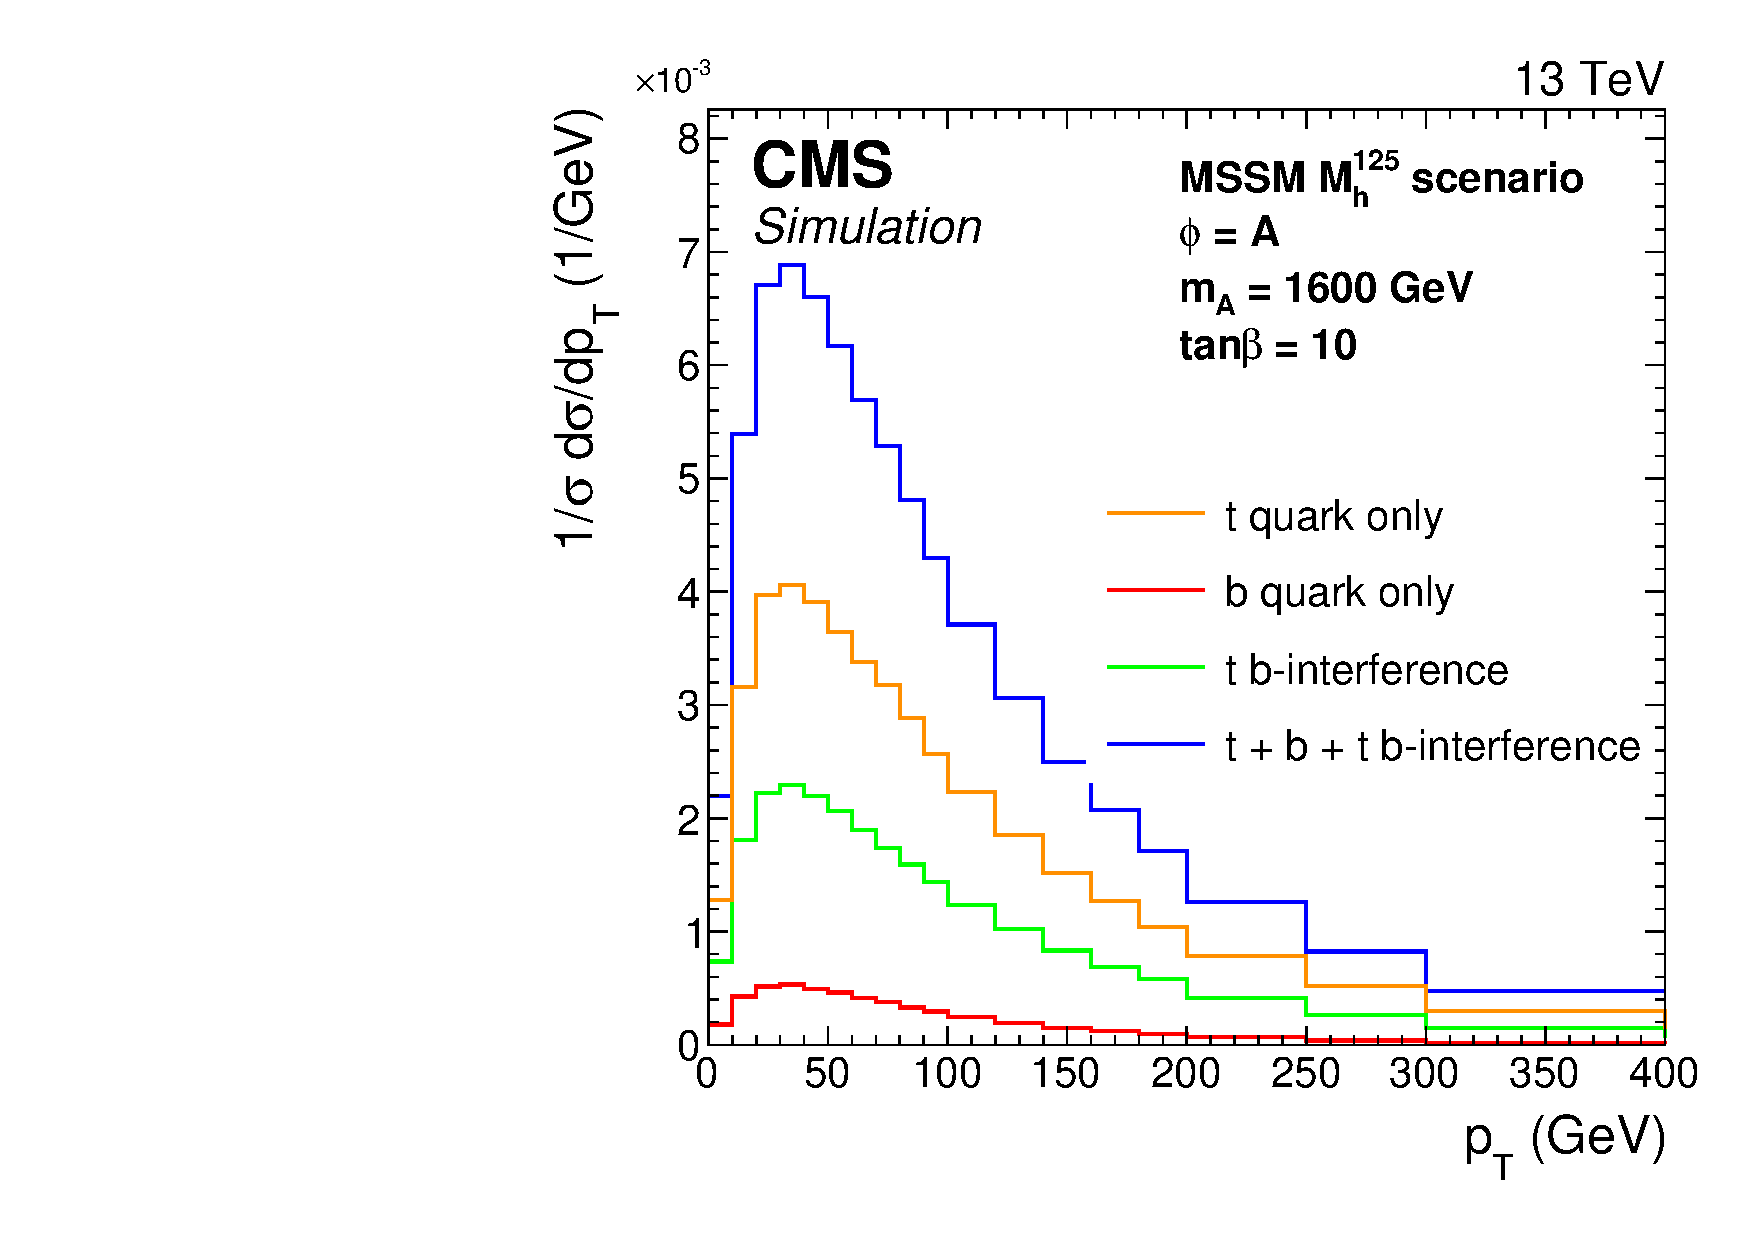
\includegraphics[width=0.5\textwidth]{Figures/pT_reweighting_plot_tanb10.pdf}}
    \subfloat[]{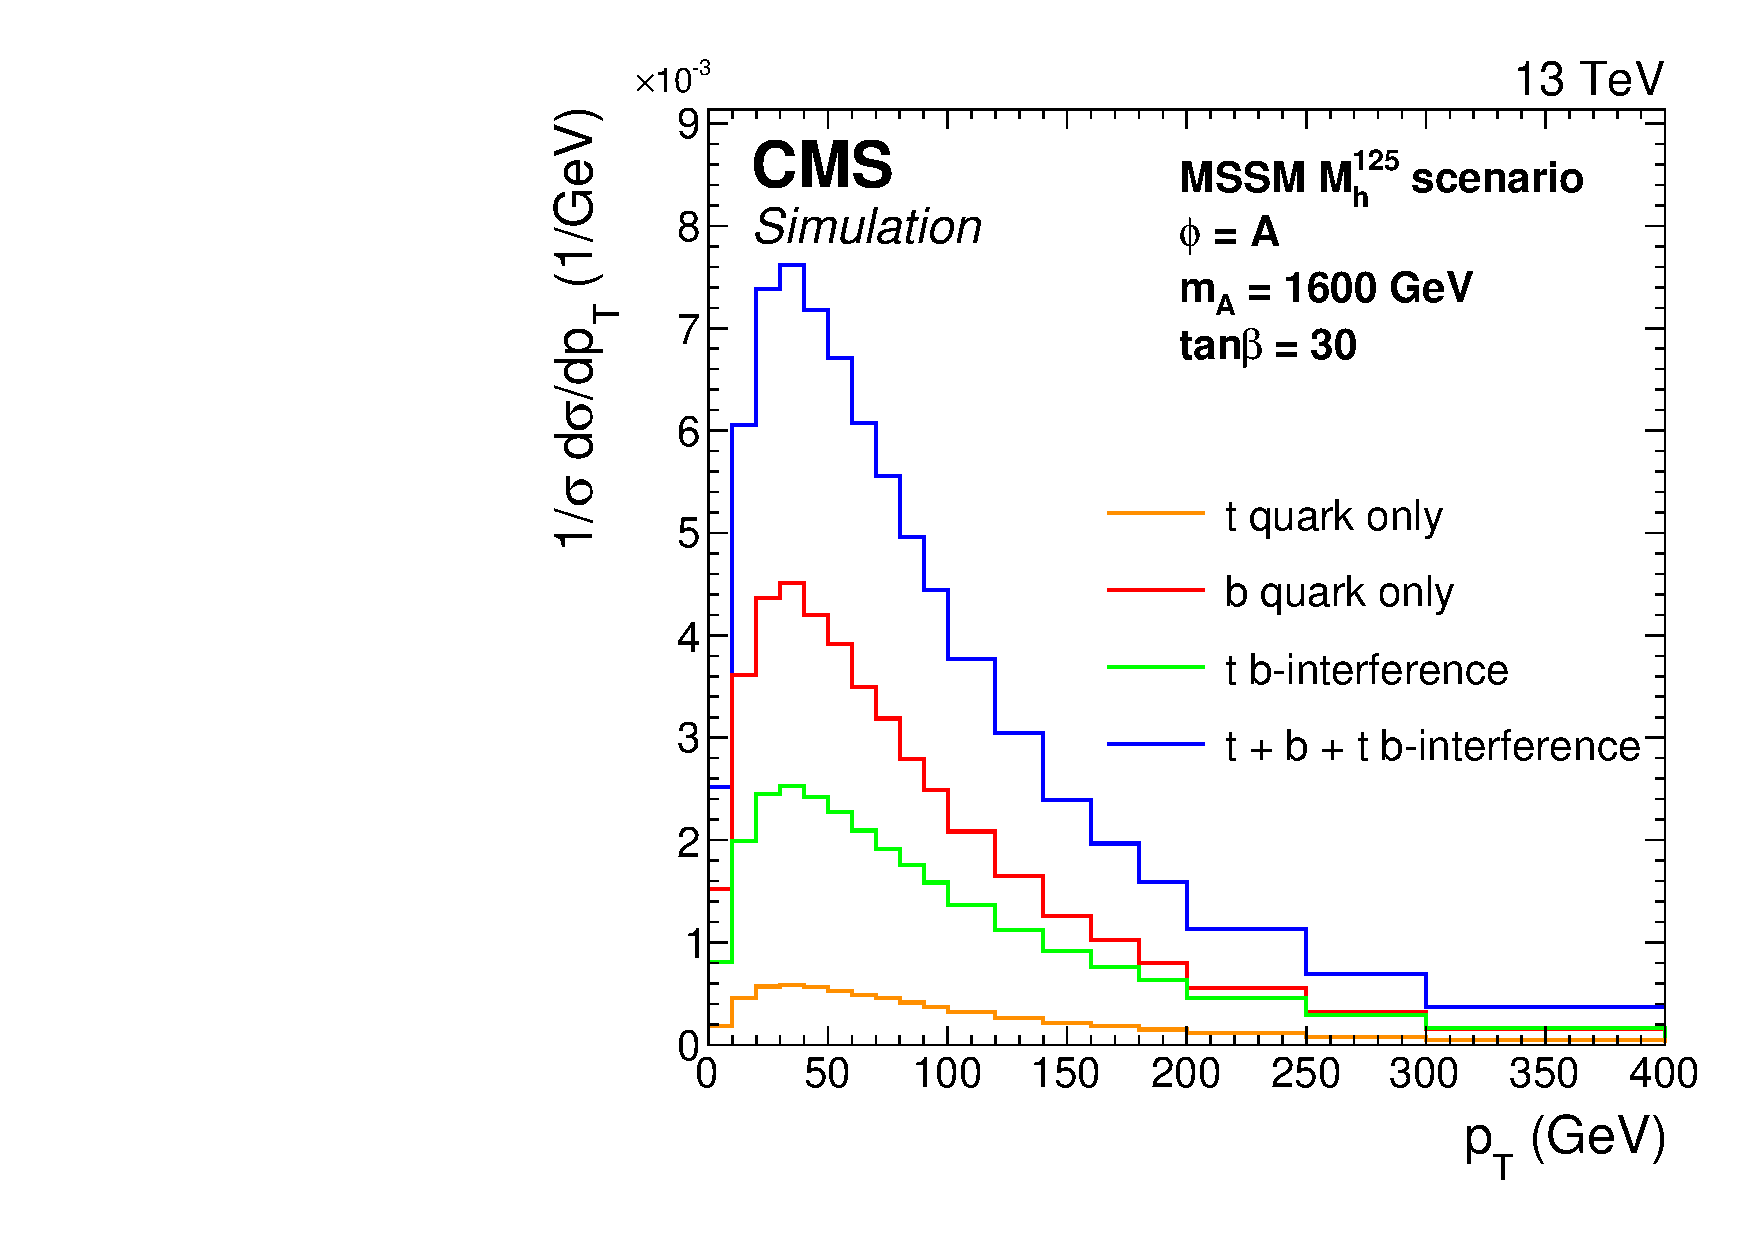
\includegraphics[width=0.5\textwidth]{Figures/pT_reweighting_plot_tanb30.pdf}}
\caption{Plots showing the $p_{T}$ density distributions of the A boson, with contributions to the gluon fusion loop displayed individually and summed. These are shown for $\tan\beta$ values of 10 (a) and 30 (b) where $m_{A} = 1600 $ GeV in the MSSM $M_{h}^{125}$ scenario.}
\label{fig:mssm_sig}
\end{figure}


\begin{figure}[!hbtp]
\centering
    \subfloat[]{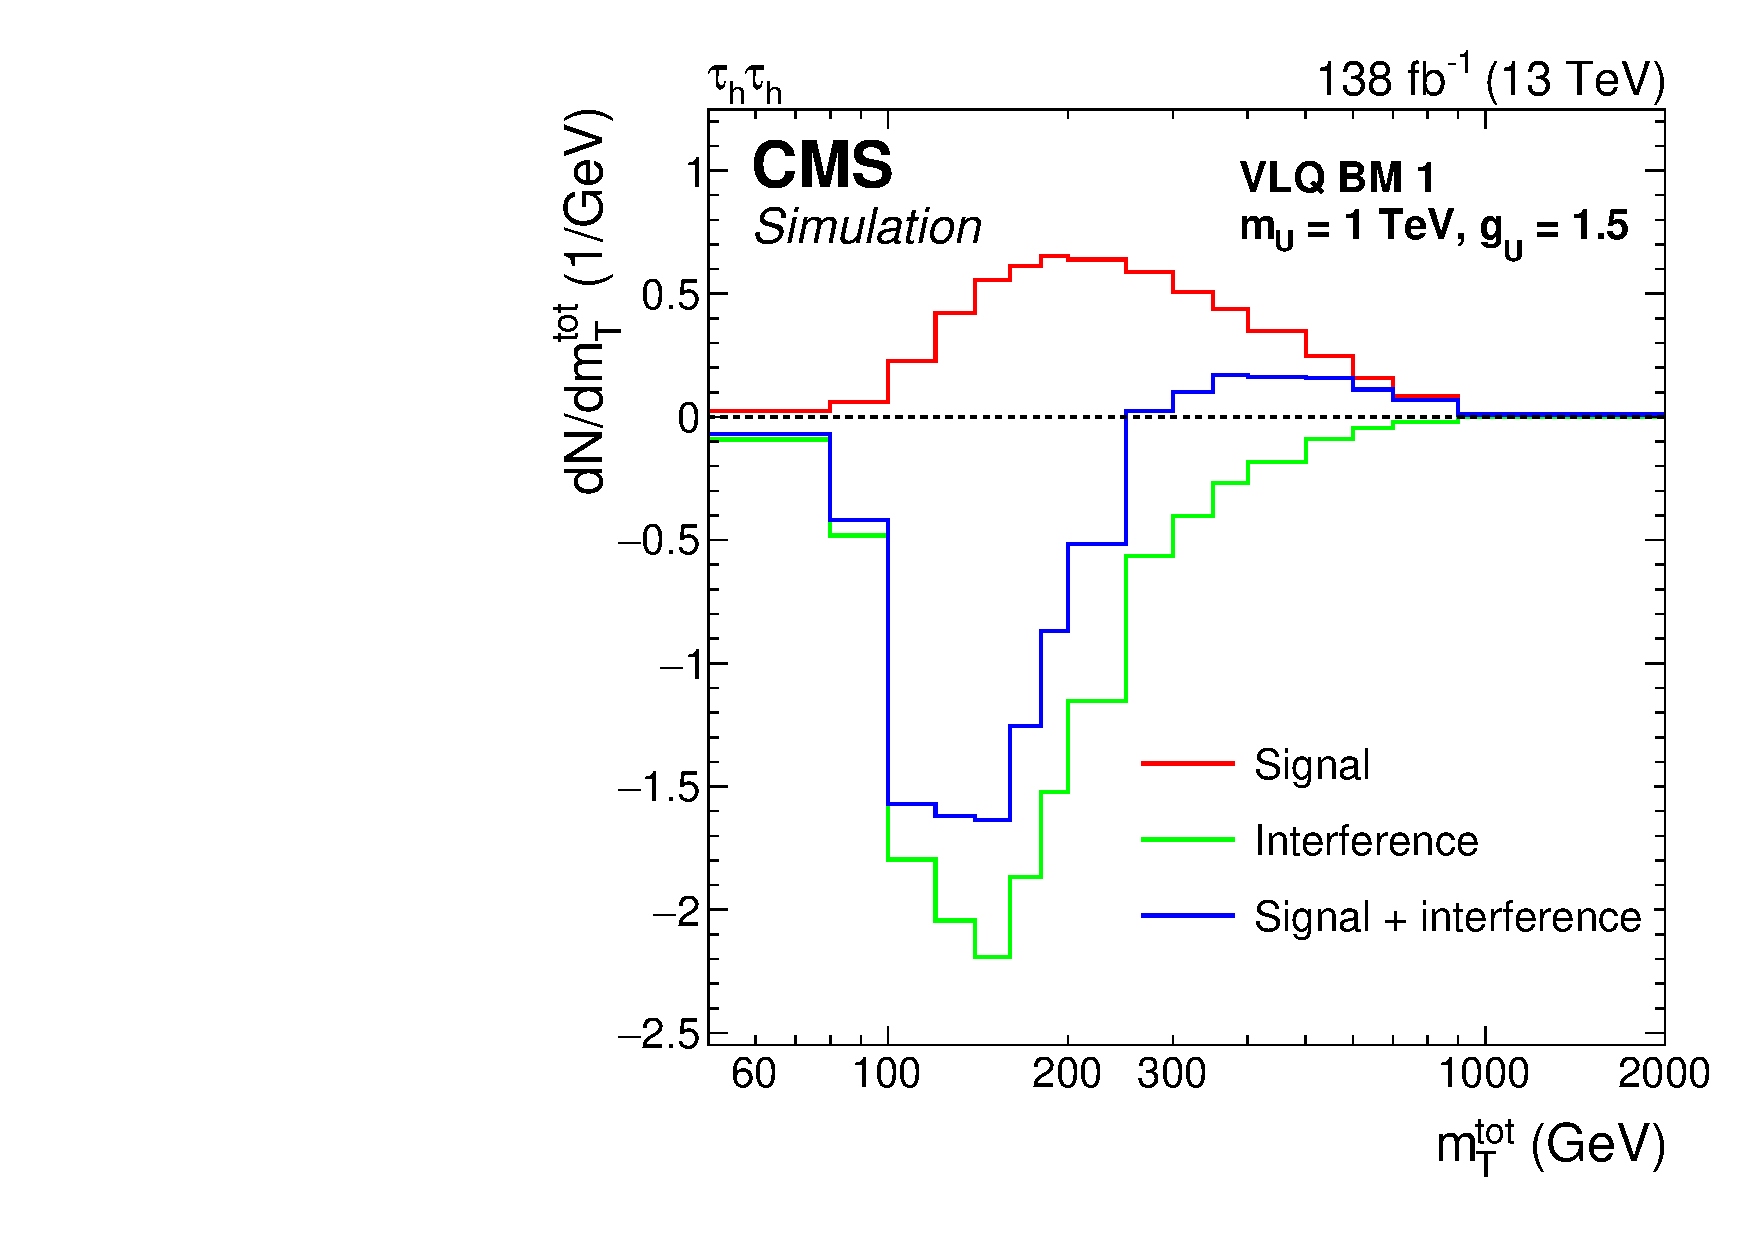
\includegraphics[width=0.5\textwidth]{Figures/vlq_signal_plot_gU1p5.pdf}}
    \subfloat[]{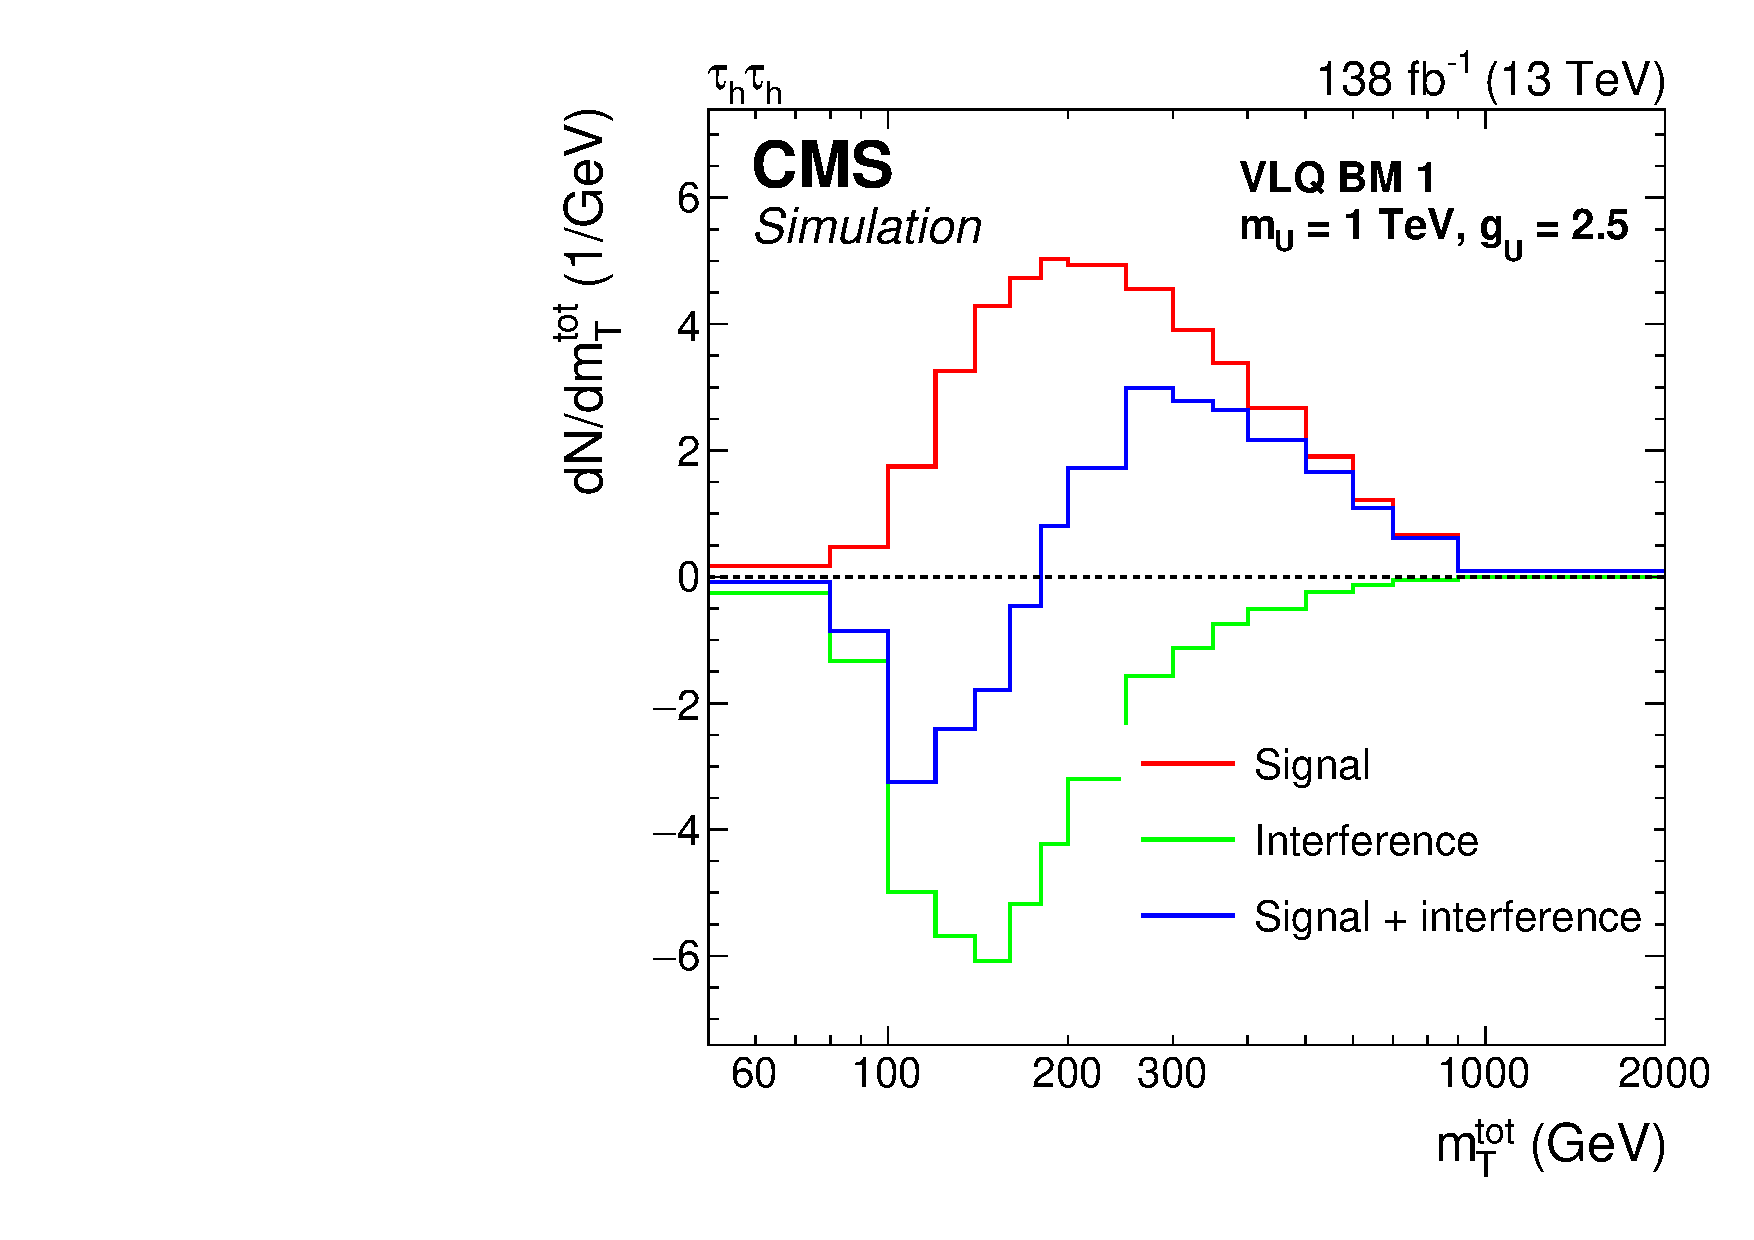
\includegraphics[width=0.5\textwidth]{Figures/vlq_signal_plot_gU2p5.pdf}}
\caption{VLQ signal.}
\label{fig:vlq_signal}
\end{figure}

\section{Event Selection}

\begin{table}[h]
    \centering
    \begin{tabular}{|c|c|}
         \hline
         Channel & Branching Fraction  \\
         \hline
         \hline
         $\tau_h \tau_h$ & 42.0\% \\
         $e \tau_h$ & 23.1\% \\
         $\mu \tau_h$ & 22.6\% \\
         $e \mu$ & 6.2\% \\
         $e e$ & 3.2\% \\
         $\mu \mu$ & 3.0\% \\
         \hline
    \end{tabular}
    \caption{}
\end{table}

\section{Signal Extraction}

Categorisation

mvis vs mttot

\section{Background Modelling Overview}

Jet fakes and genuine taus.

Explain MC generators.

Overview data driven methods.

Fractions of processes in each channel.

\section{Embedding Method}

\begin{figure}[!hbtp]
\centering
    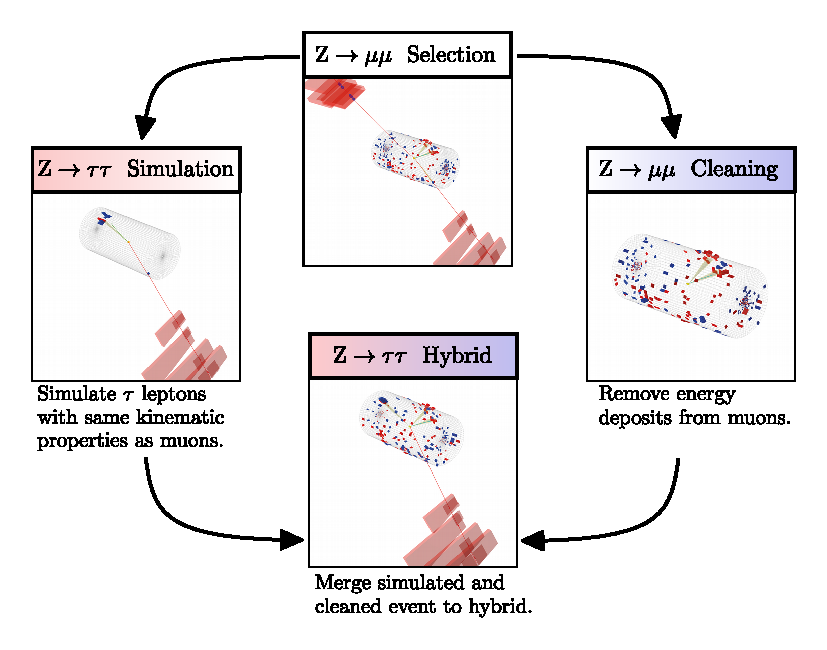
\includegraphics[width=0.8\textwidth]{Figures/Embedding_Diagram.pdf}
\caption{Embedding.}
\label{fig:embedding}
\end{figure}

Validation plots of it working

\section{Fake Factor Method}

Overview

\subsection{Determination Regions}

\begin{figure}[!hbtp]
\centering
    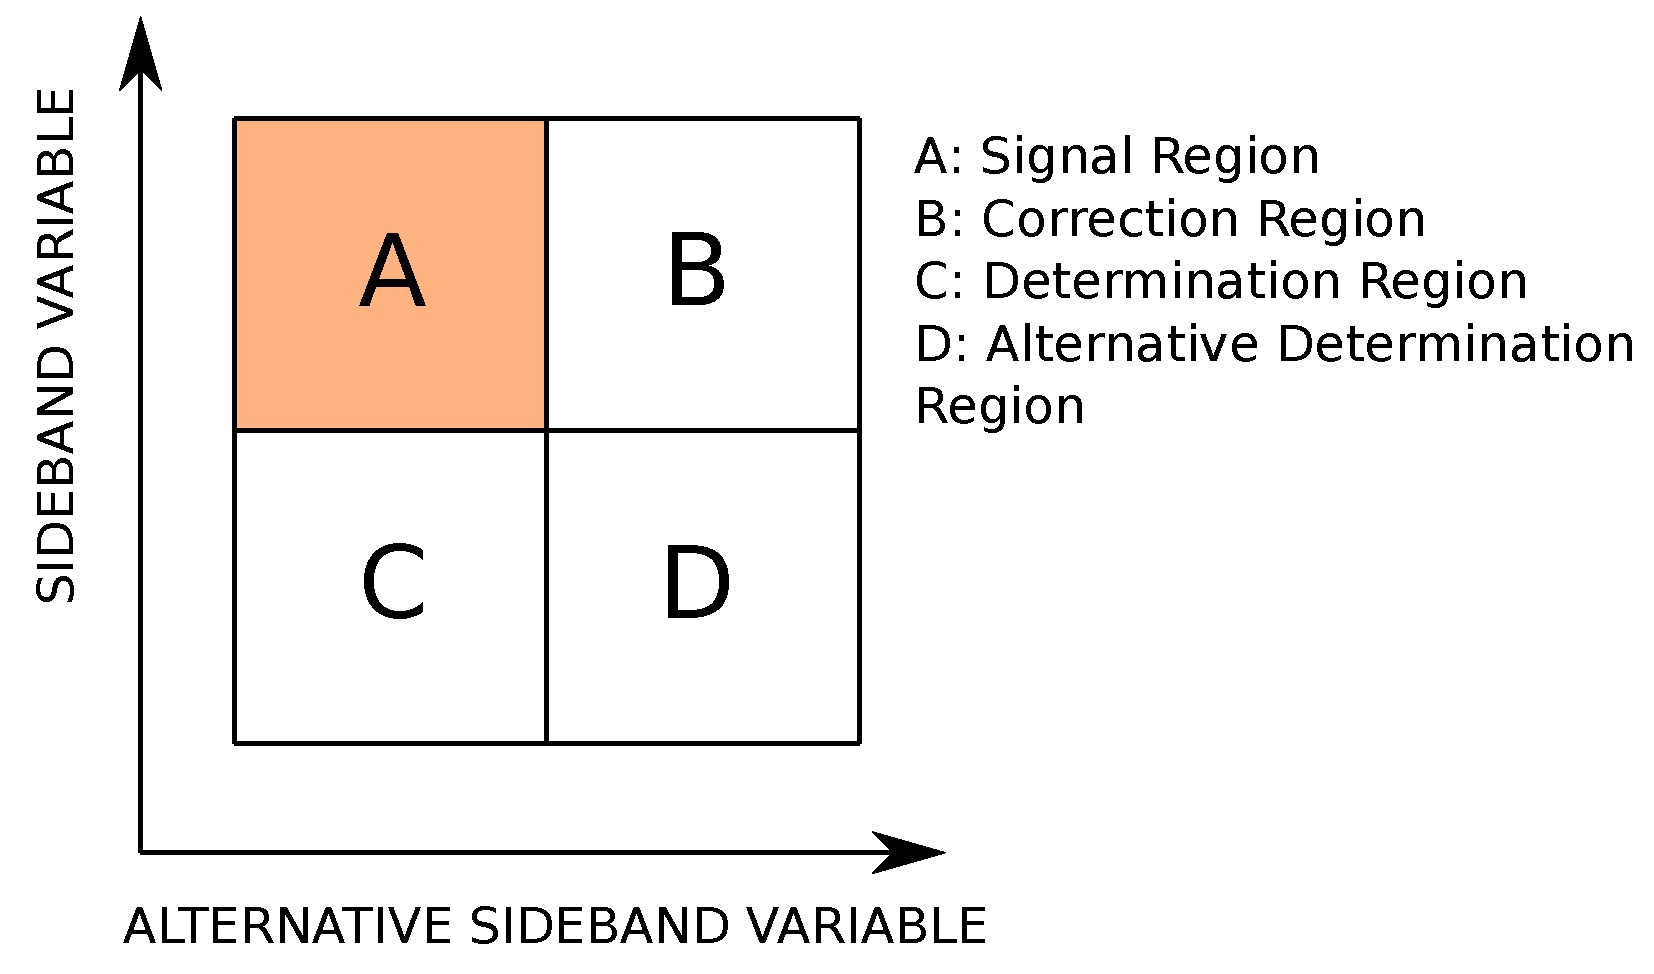
\includegraphics[width=0.8\textwidth]{Figures/ff_diagram.pdf}
\caption{FF diagram.}
\label{fig:ff_schematic}
\end{figure}

\subsection{Parametrisation}

\begin{figure}[!hbtp]
\centering
    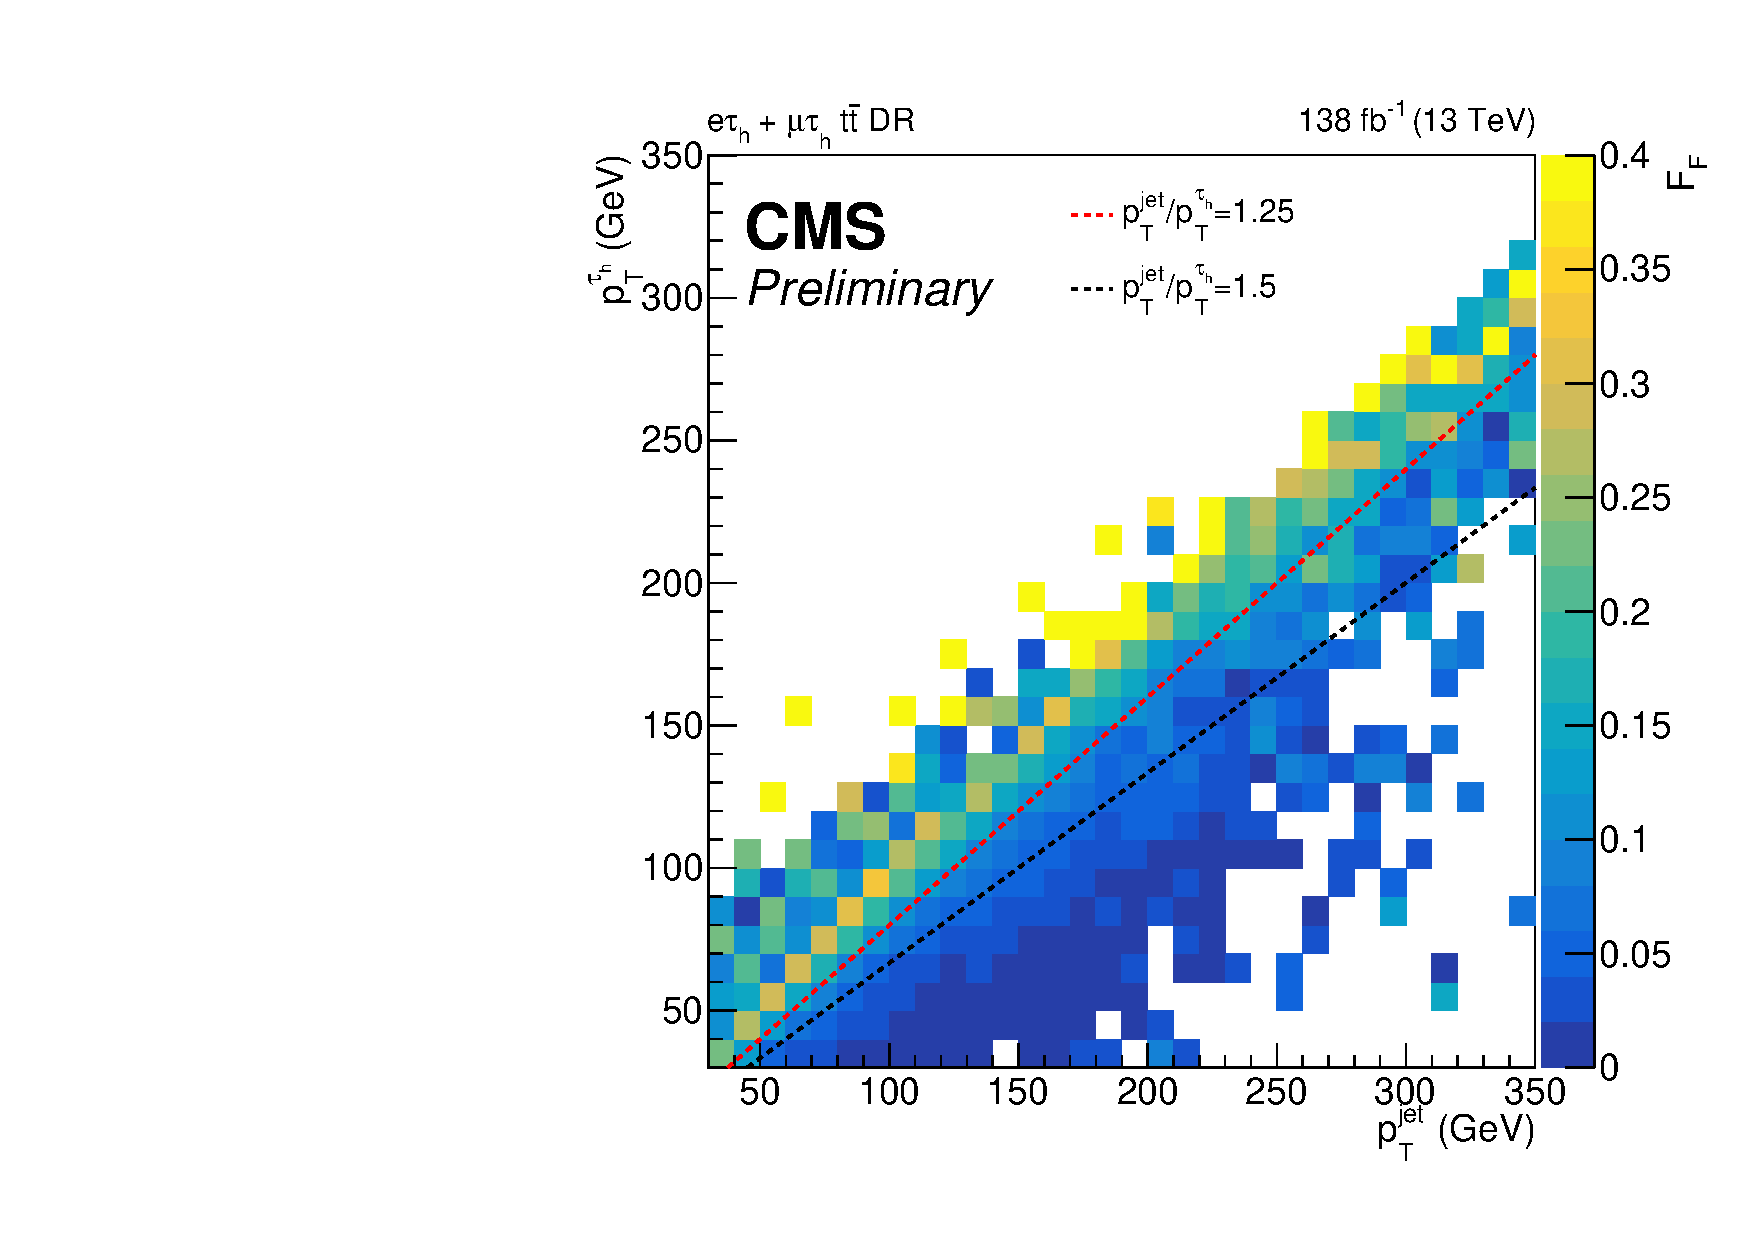
\includegraphics[width=0.6\textwidth]{Figures/ff_colz_ttbar_lt.pdf}
\caption{FF colz.}
\label{fig:ff_colz}
\end{figure}

fits

\subsection{Corrections}

fits

\subsection{Appilcation Region Fractions}


\subsection{Applying Fake Factors}

using leading tau
subtracting off rest
w fakes in tt

\section{Uncertainty Model}

bulleted list of uncertainties used in the analysis.

\section{Postfit Plots}

\begin{figure}[!hbtp]
\centering
    \subfloat[]{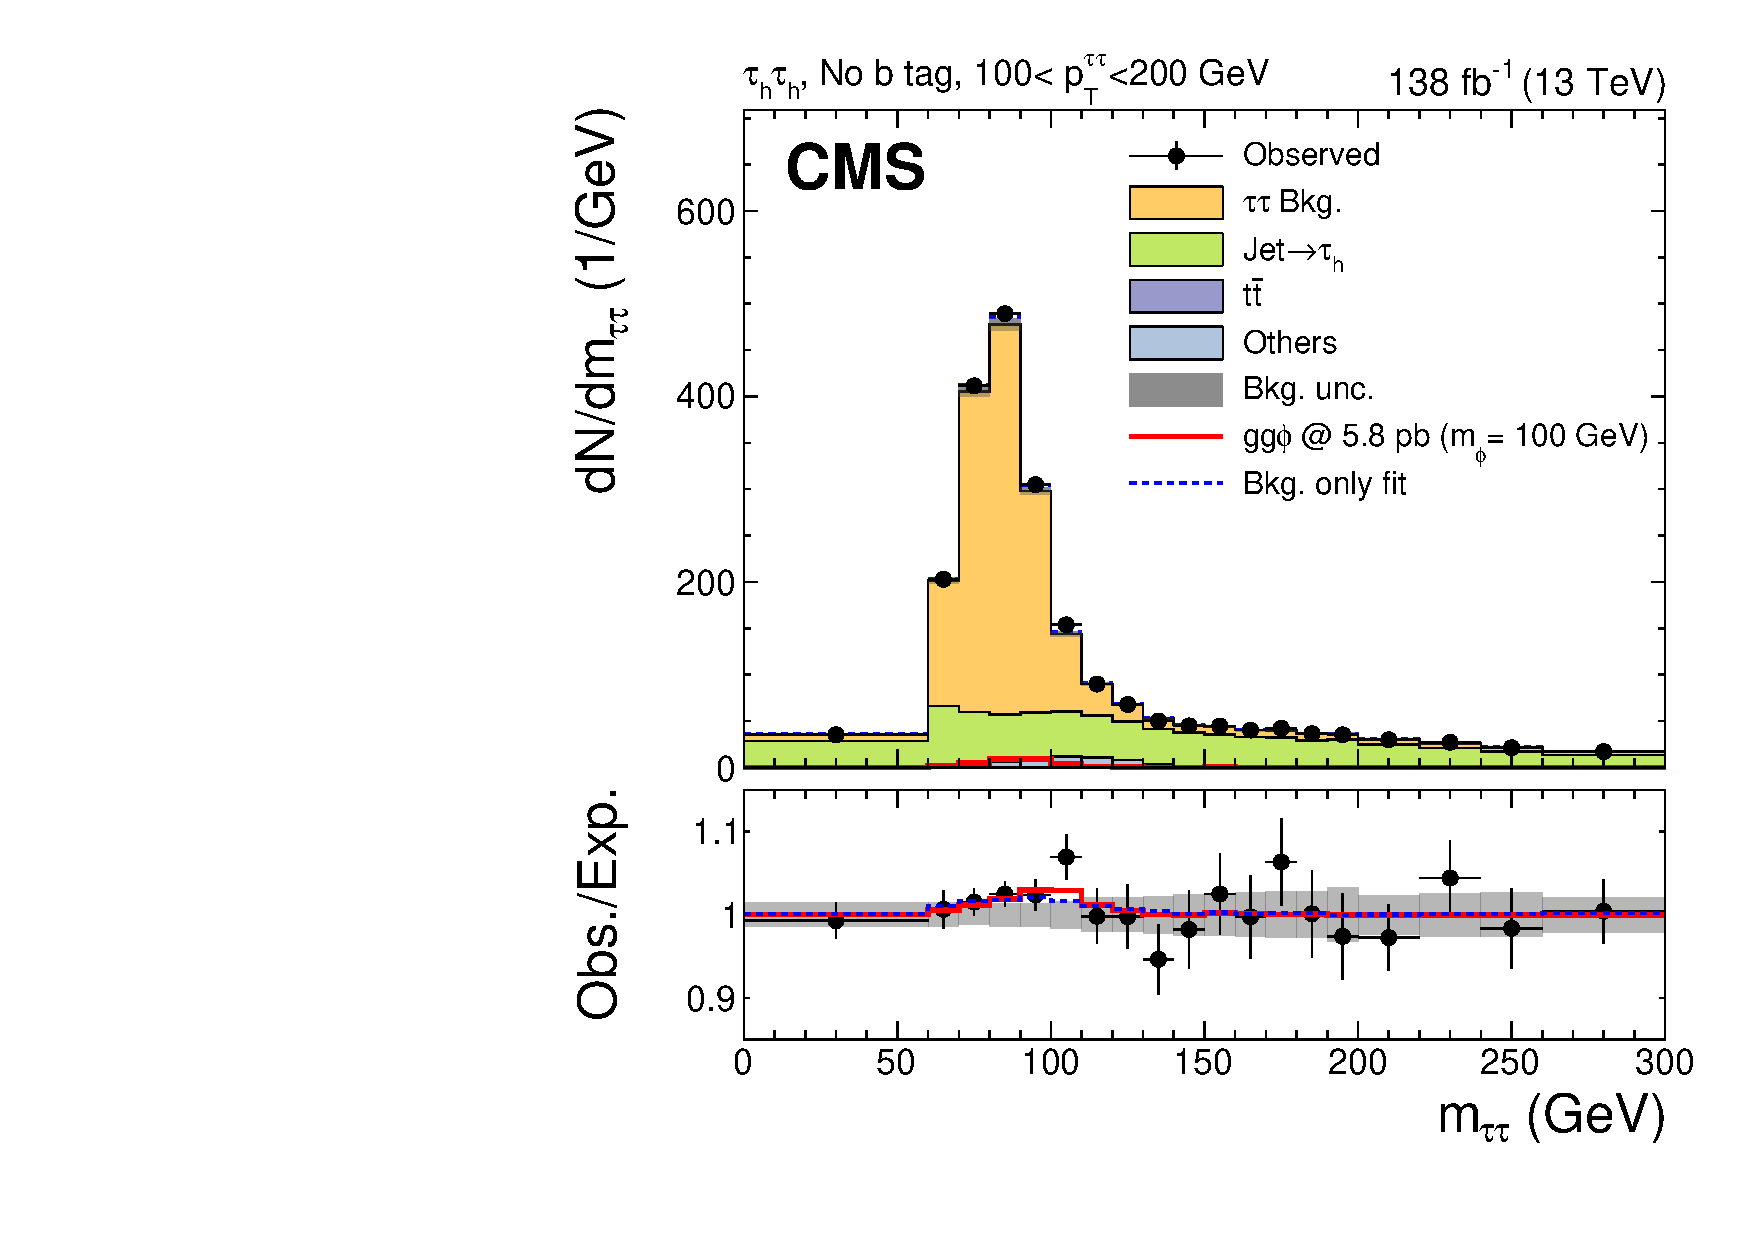
\includegraphics[width=0.45\textwidth]{Figures/postfit_lowmass_tt_nobtag_mediumpT.pdf}}
    \subfloat[]{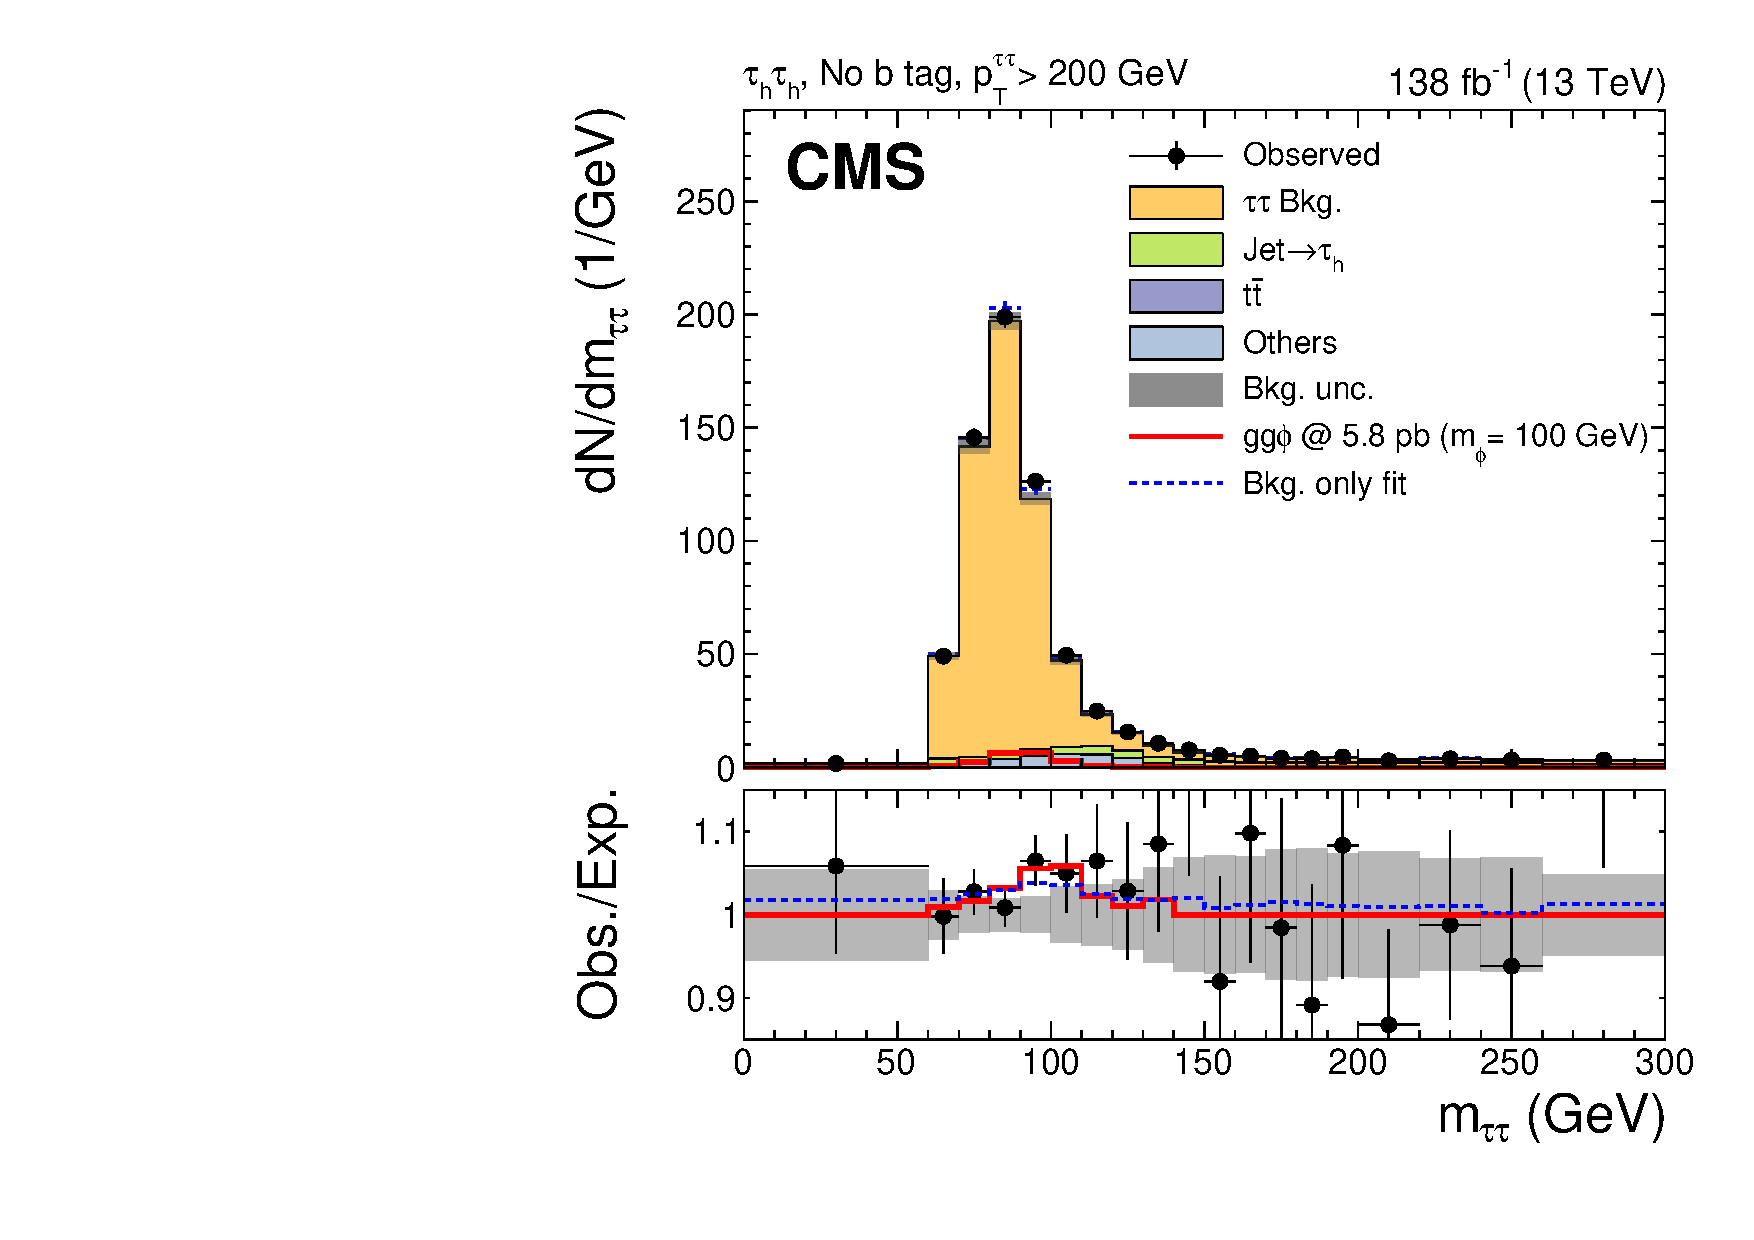
\includegraphics[width=0.45\textwidth]{Figures/postfit_lowmass_tt_nobtag_highpT.pdf}} \\
    \subfloat[]{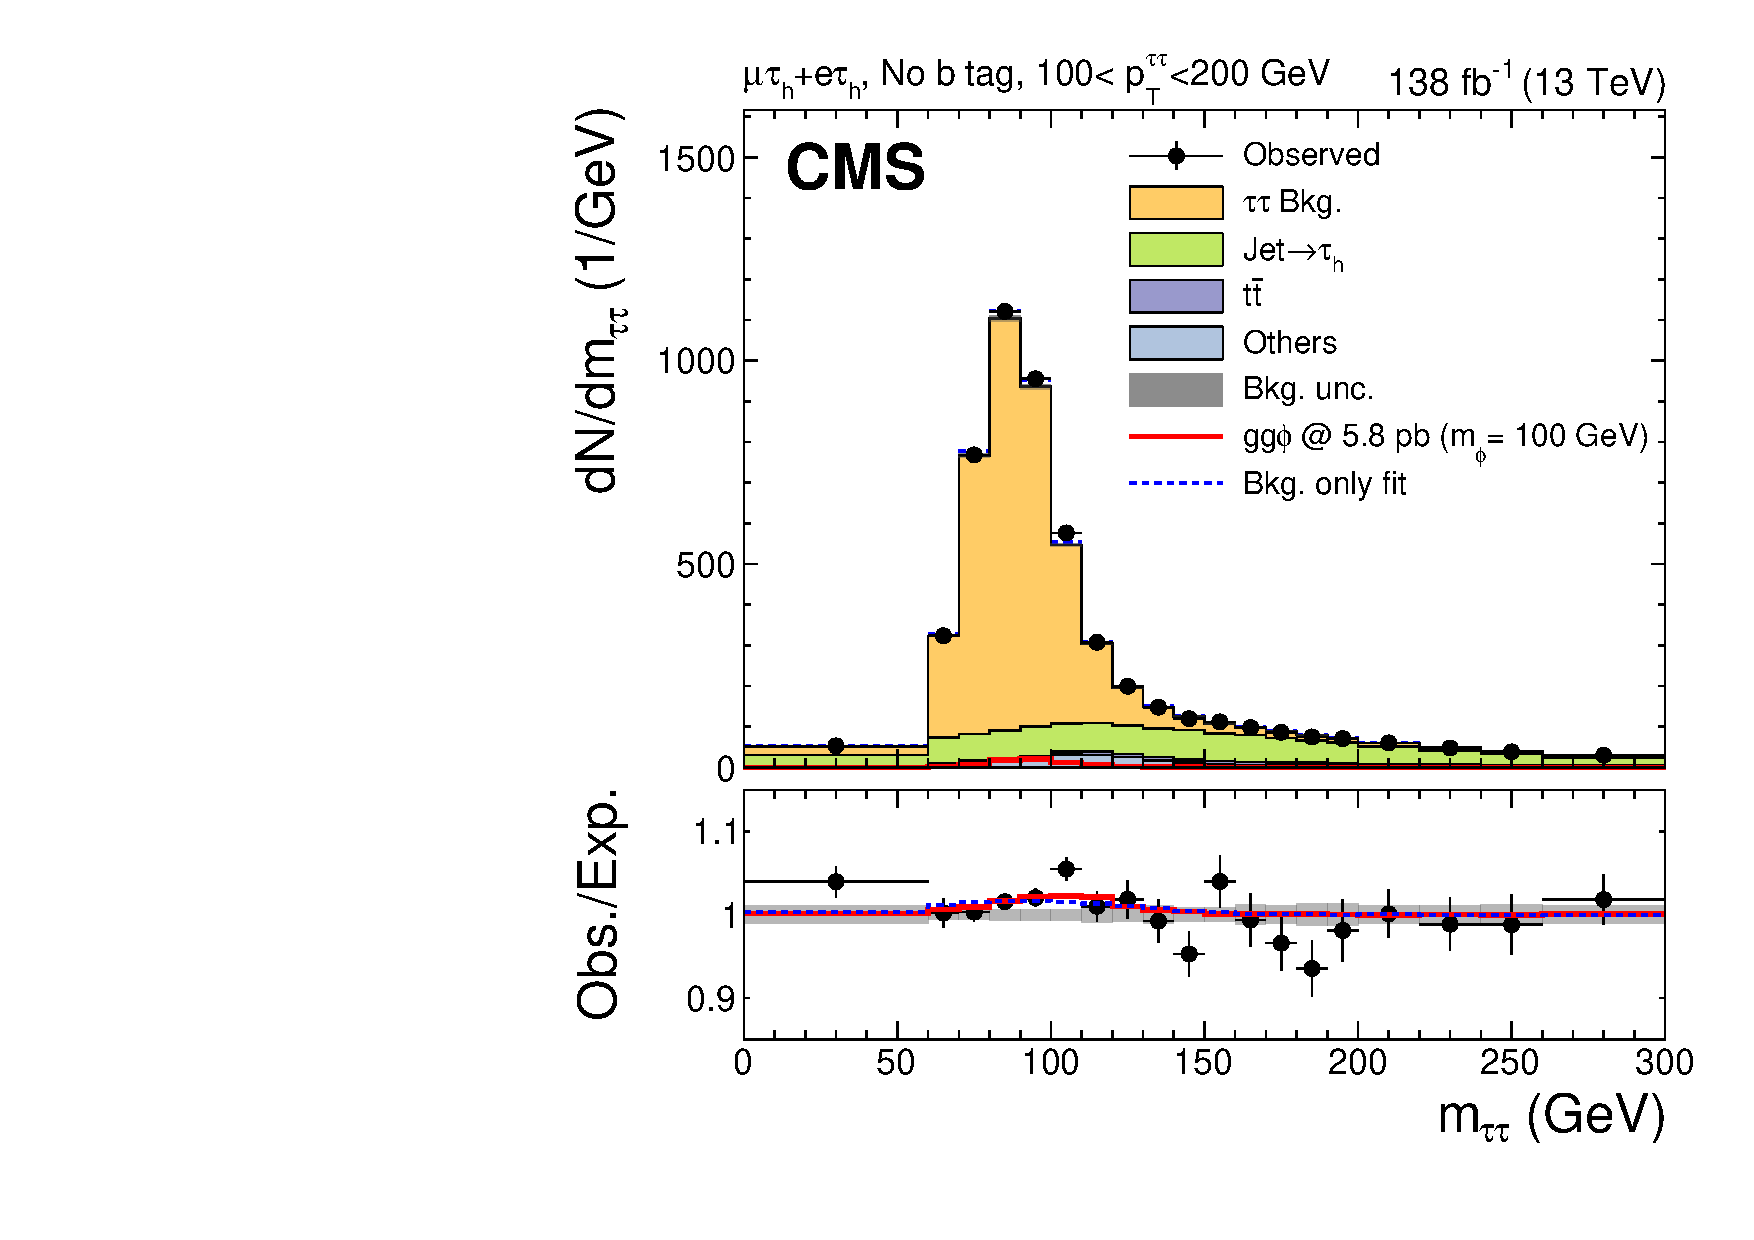
\includegraphics[width=0.45\textwidth]{Figures/postfit_lowmass_lt_nobtag_mediumpT.pdf}}
    \subfloat[]{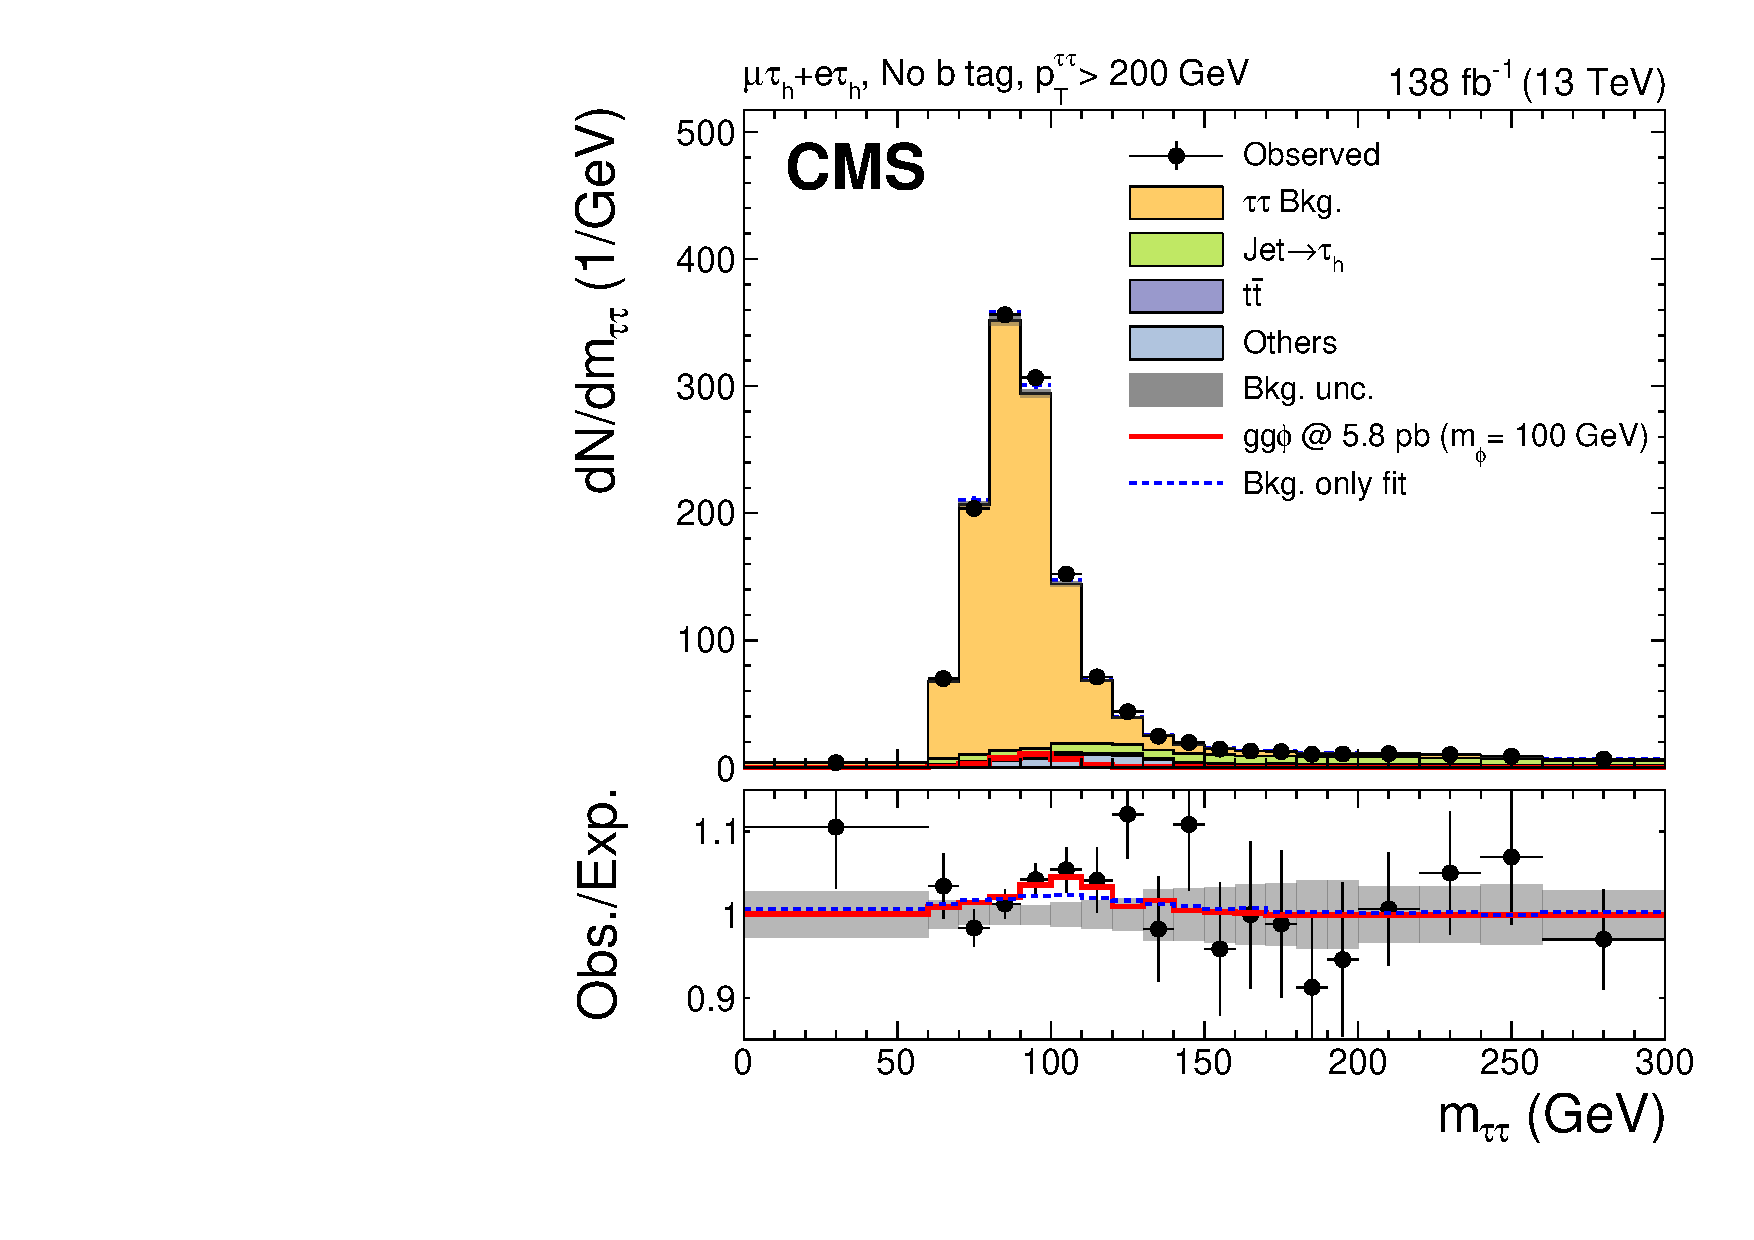
\includegraphics[width=0.45\textwidth]{Figures/postfit_lowmass_lt_nobtag_highpT.pdf}} \\
    \subfloat[]{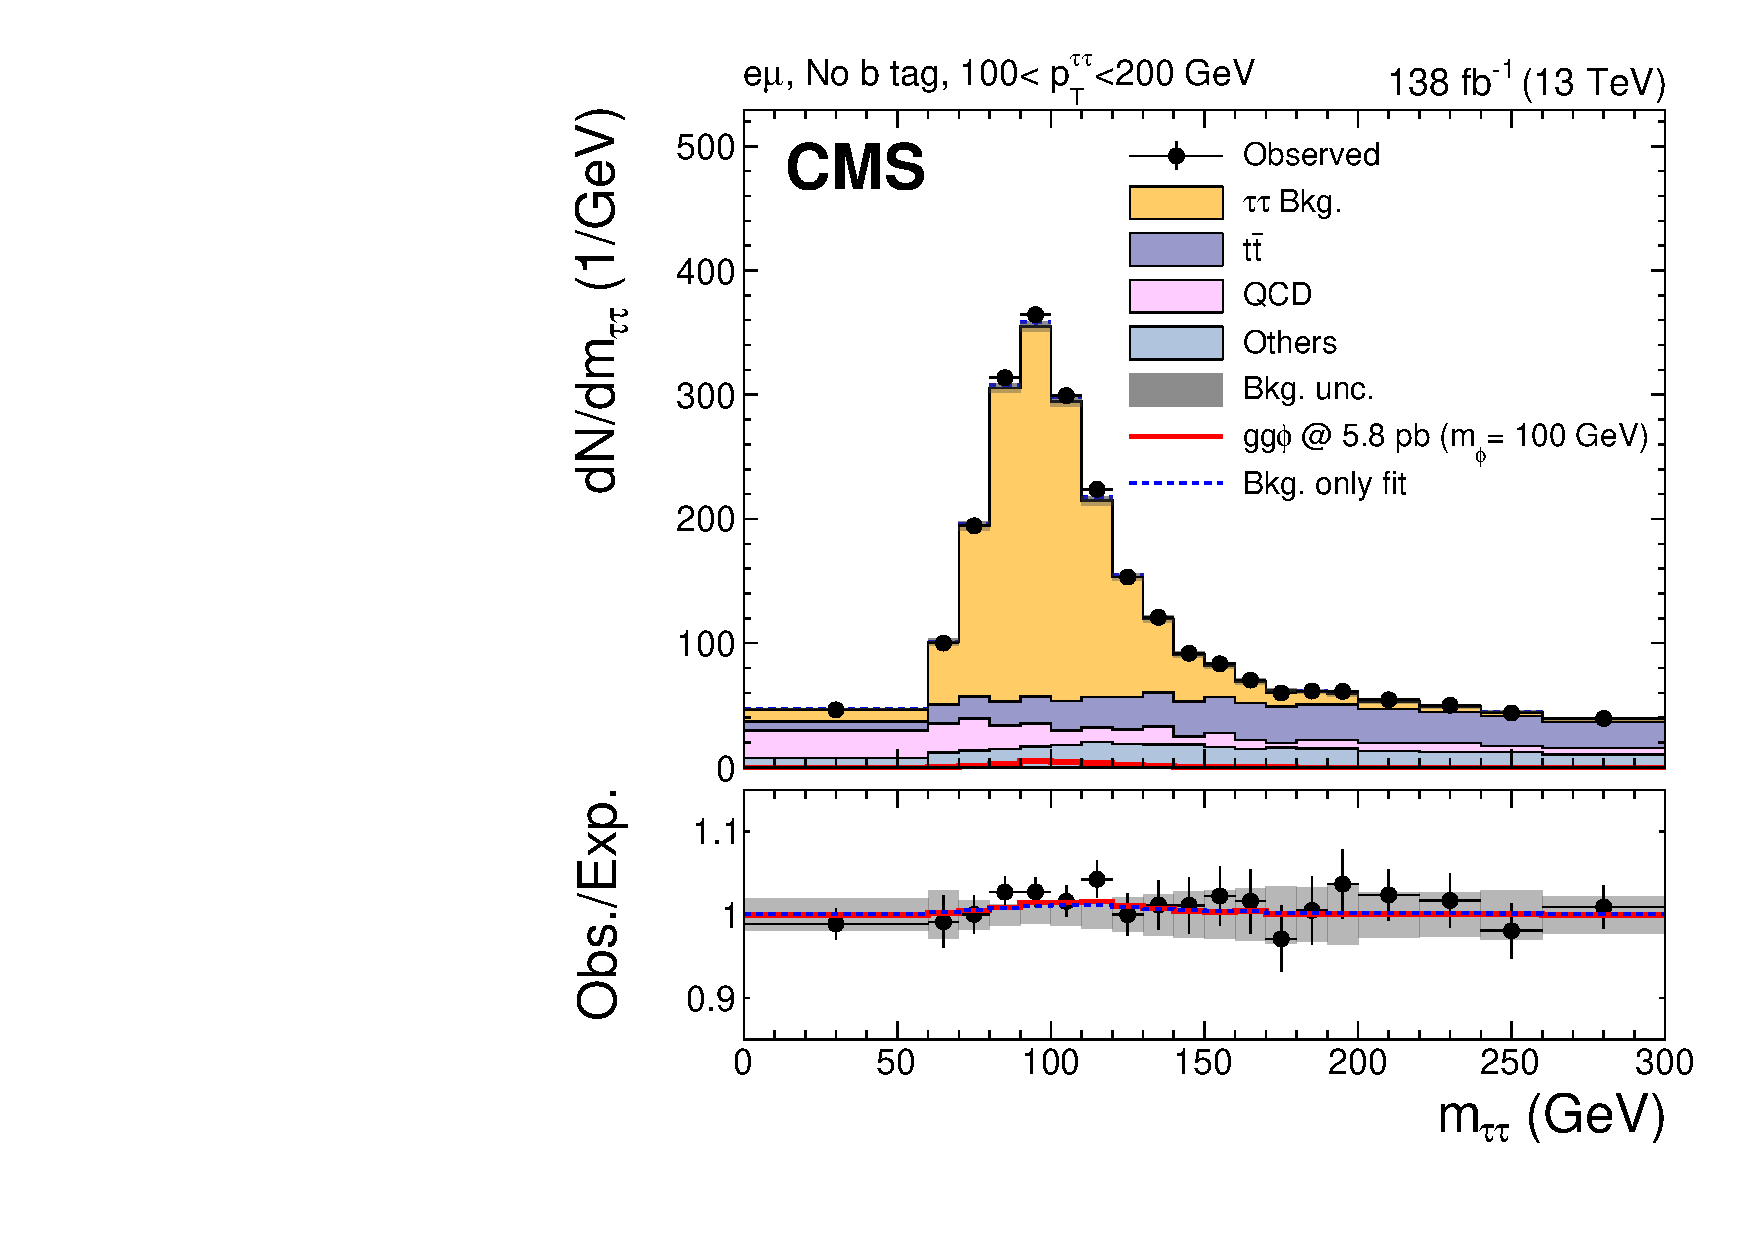
\includegraphics[width=0.45\textwidth]{Figures/postfit_lowmass_em_nobtag_mediumpT.pdf}}
    \subfloat[]{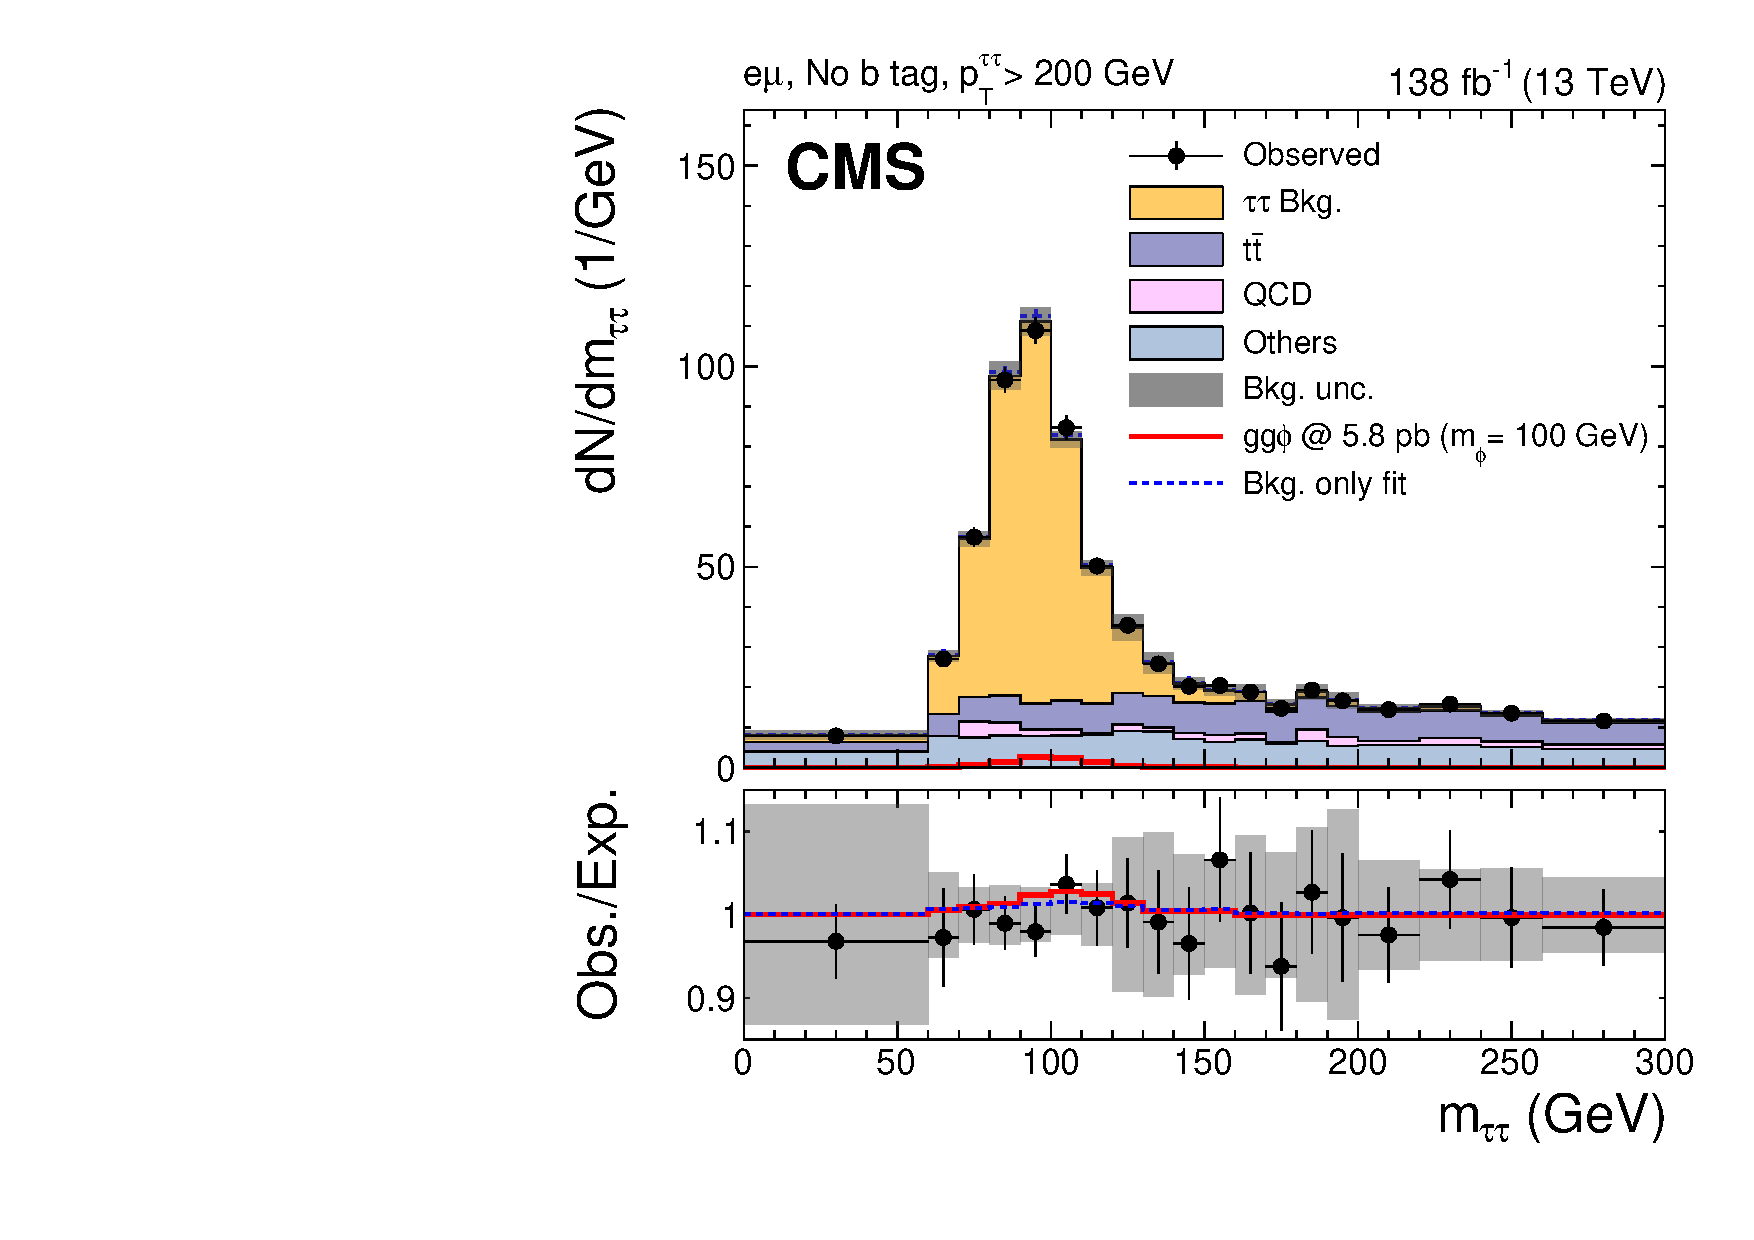
\includegraphics[width=0.45\textwidth]{Figures/postfit_lowmass_em_nobtag_highpT.pdf}}
\caption{Low mass postfit.}
\label{fig:low_mass_postfit}
\end{figure}

\begin{figure}[!hbtp]
\centering
    \subfloat[]{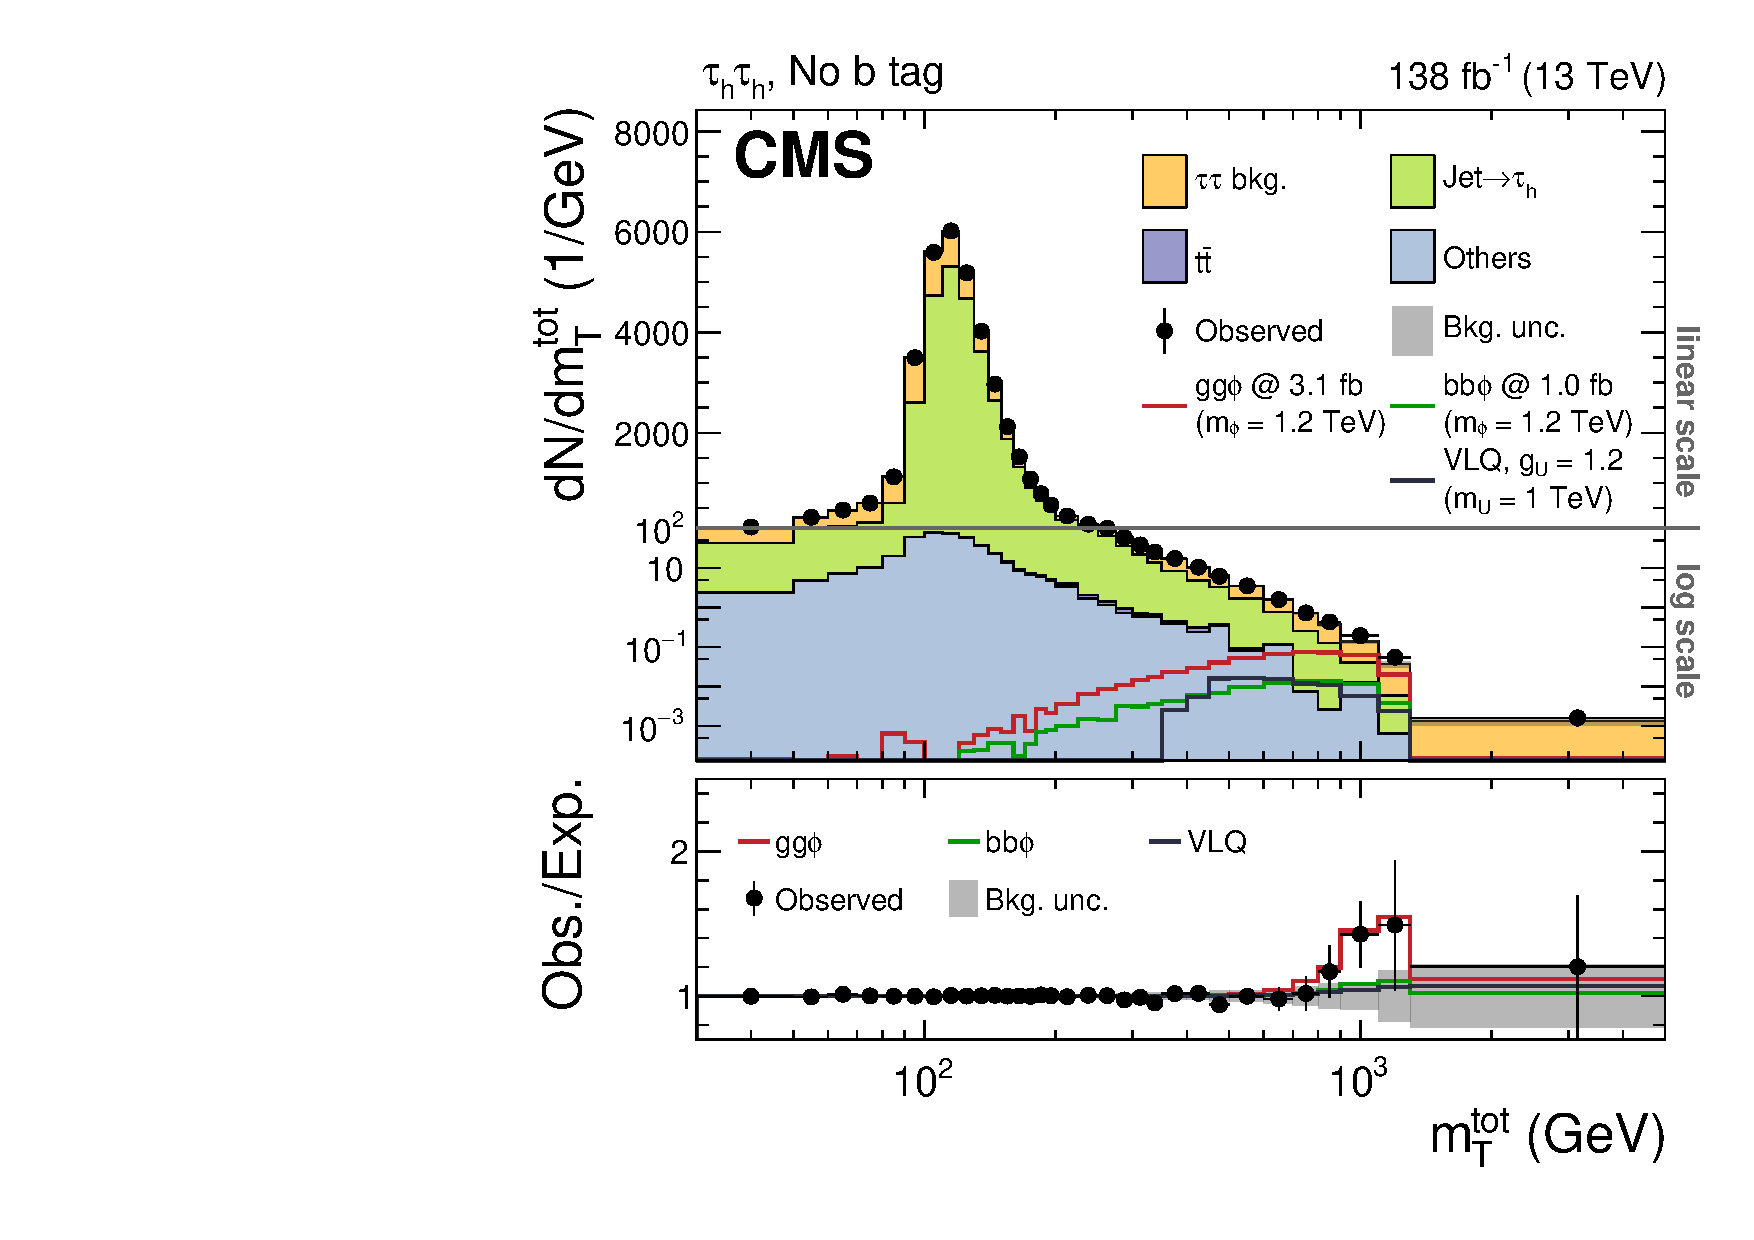
\includegraphics[width=0.45\textwidth]{Figures/postfit_highmass_tt_nobtag.pdf}}
    \subfloat[]{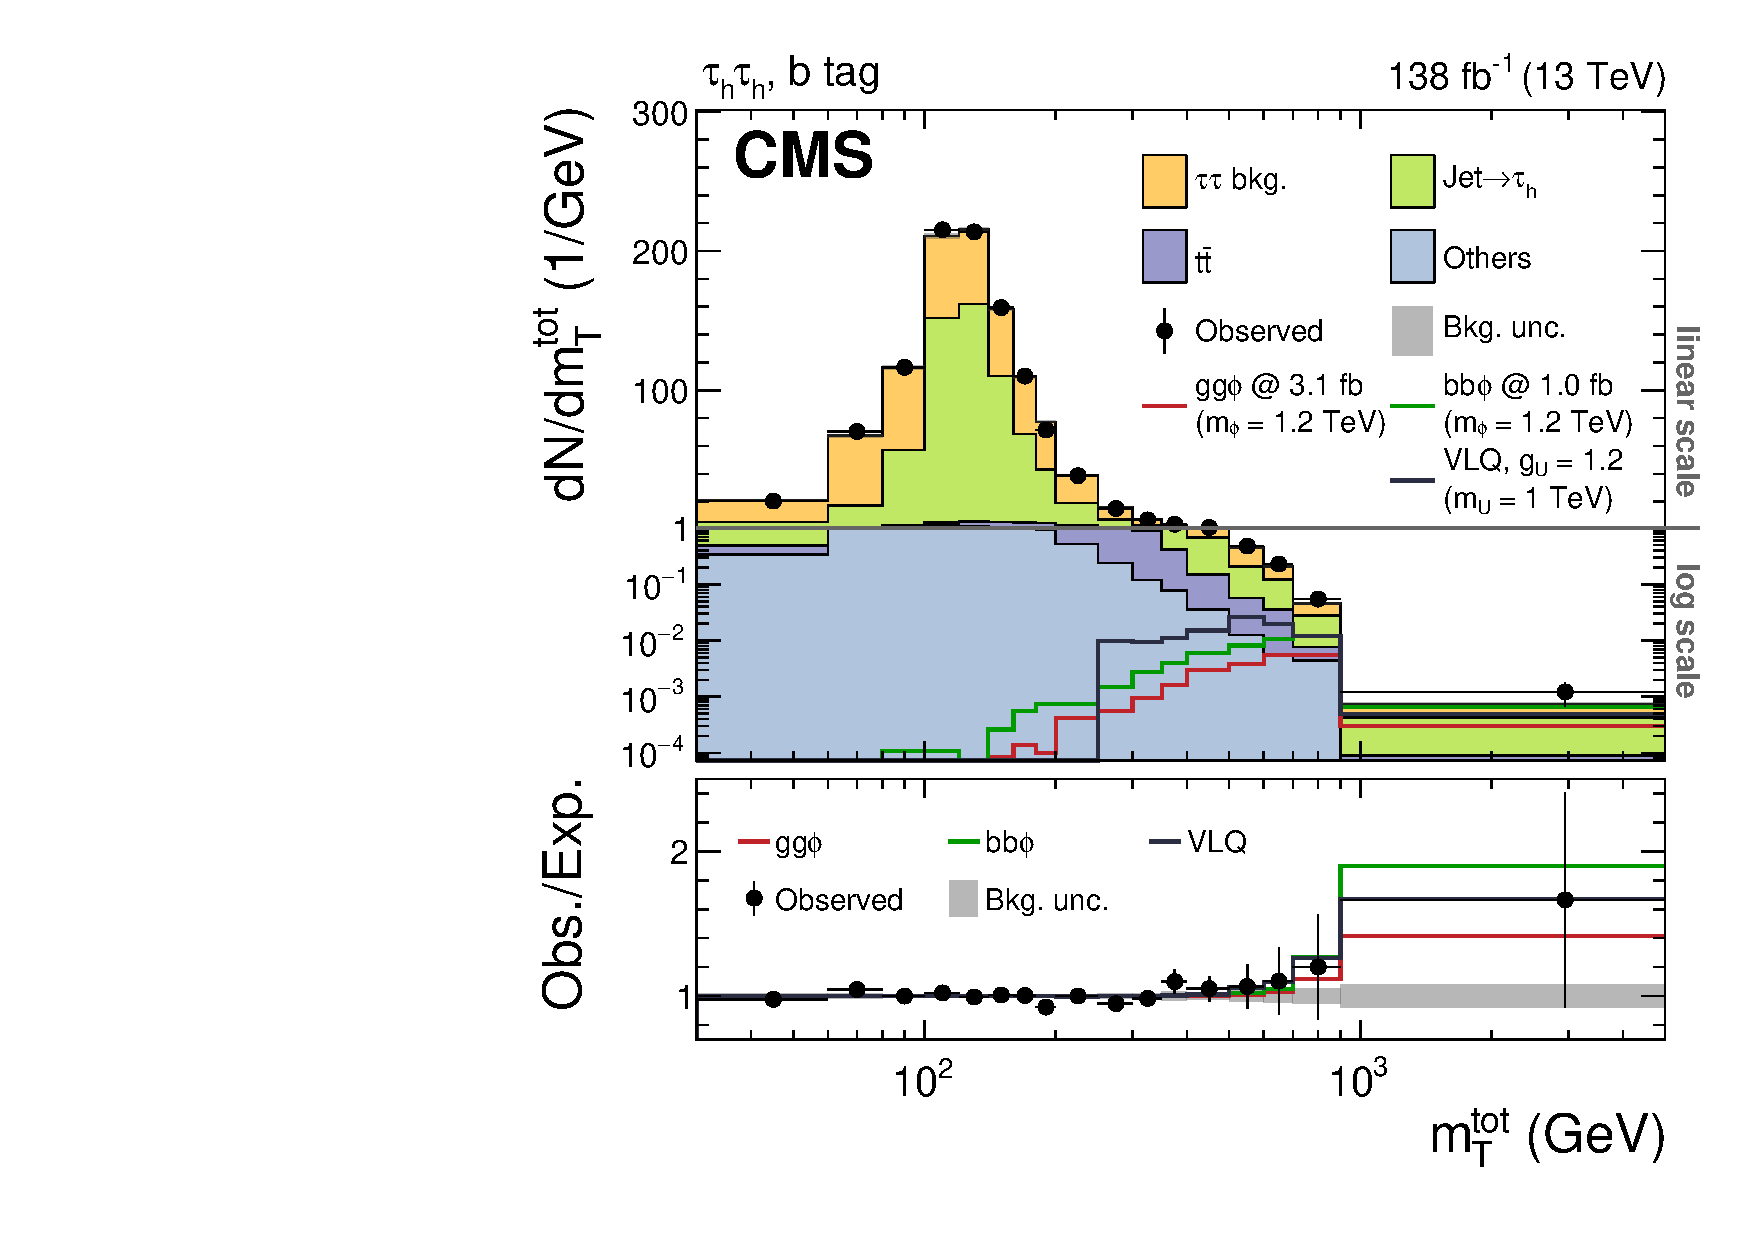
\includegraphics[width=0.45\textwidth]{Figures/postfit_highmass_tt_btag.pdf}} \\
    \subfloat[]{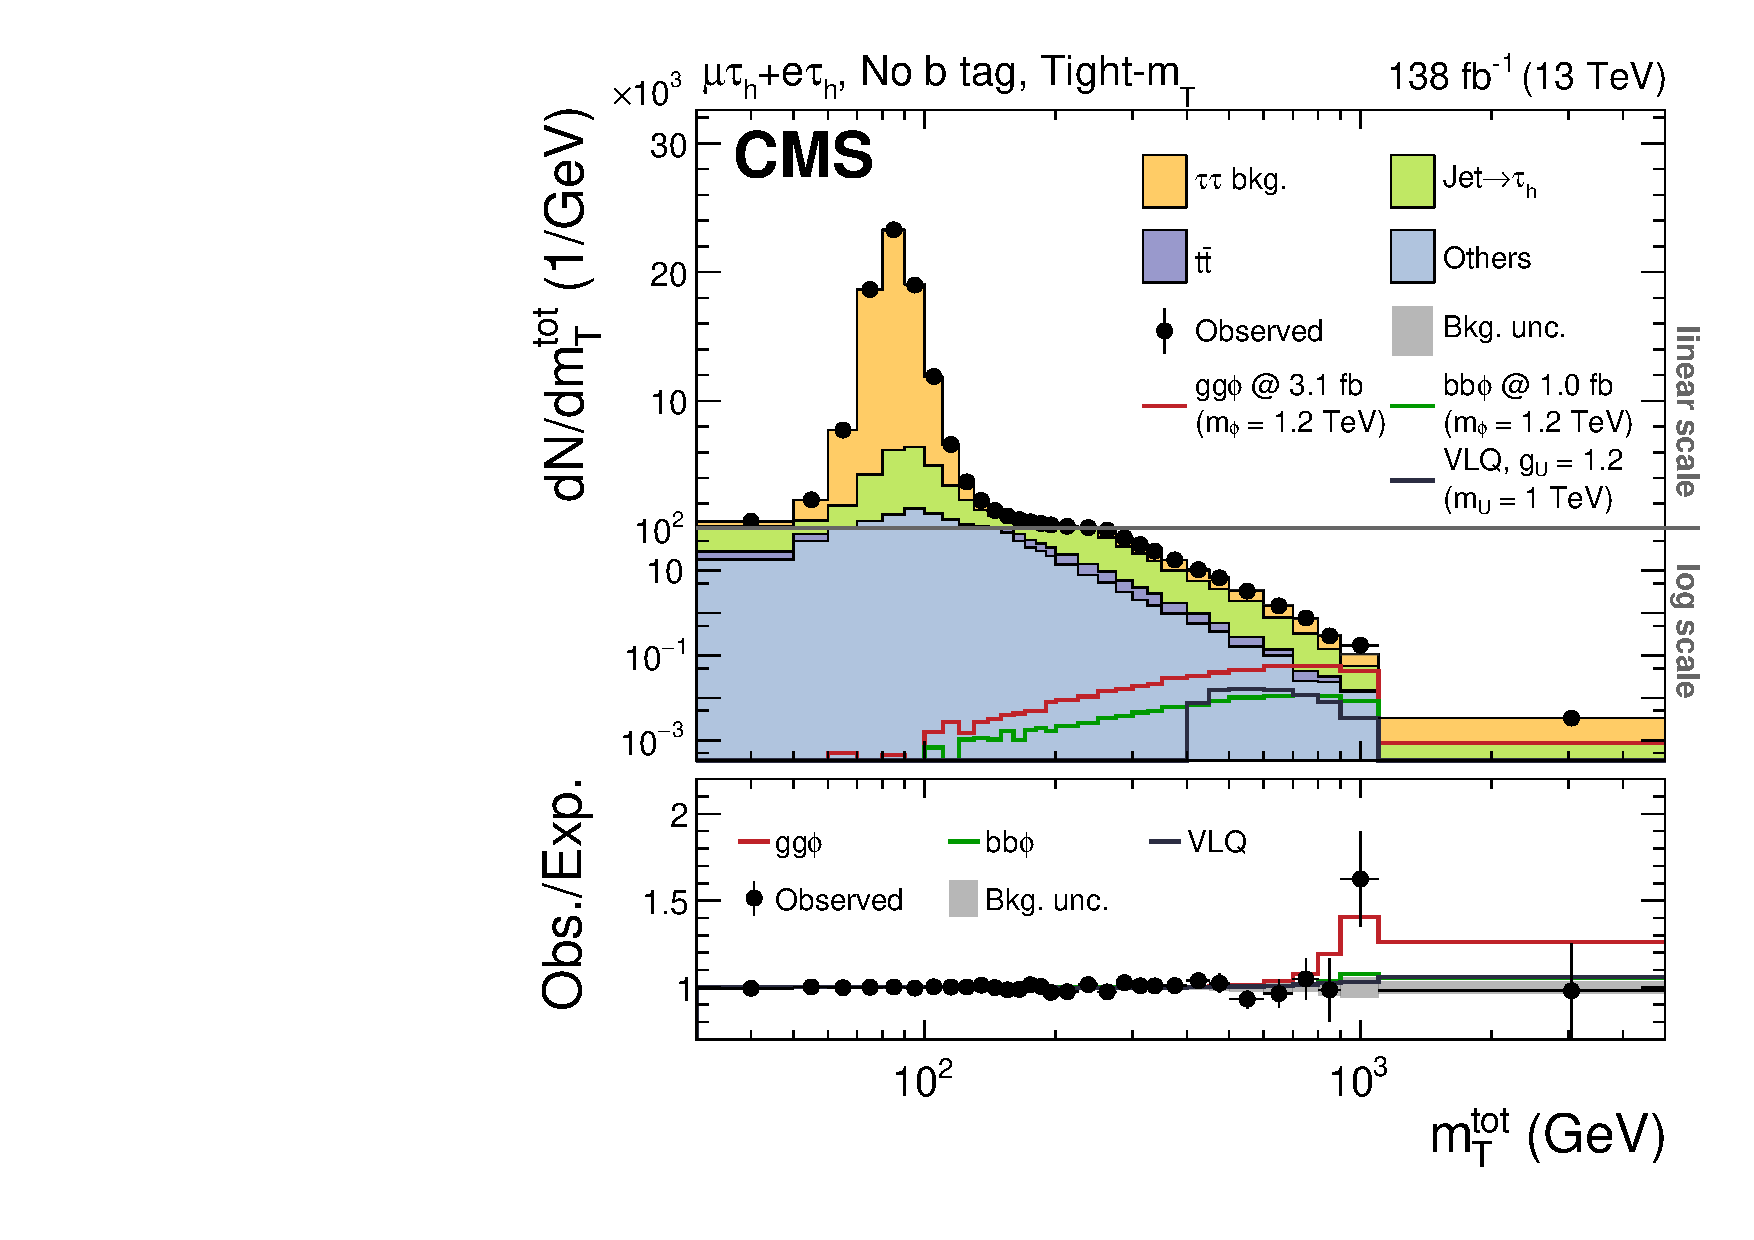
\includegraphics[width=0.45\textwidth]{Figures/postfit_highmass_lt_nobtag_tightmT.pdf}}
    \subfloat[]{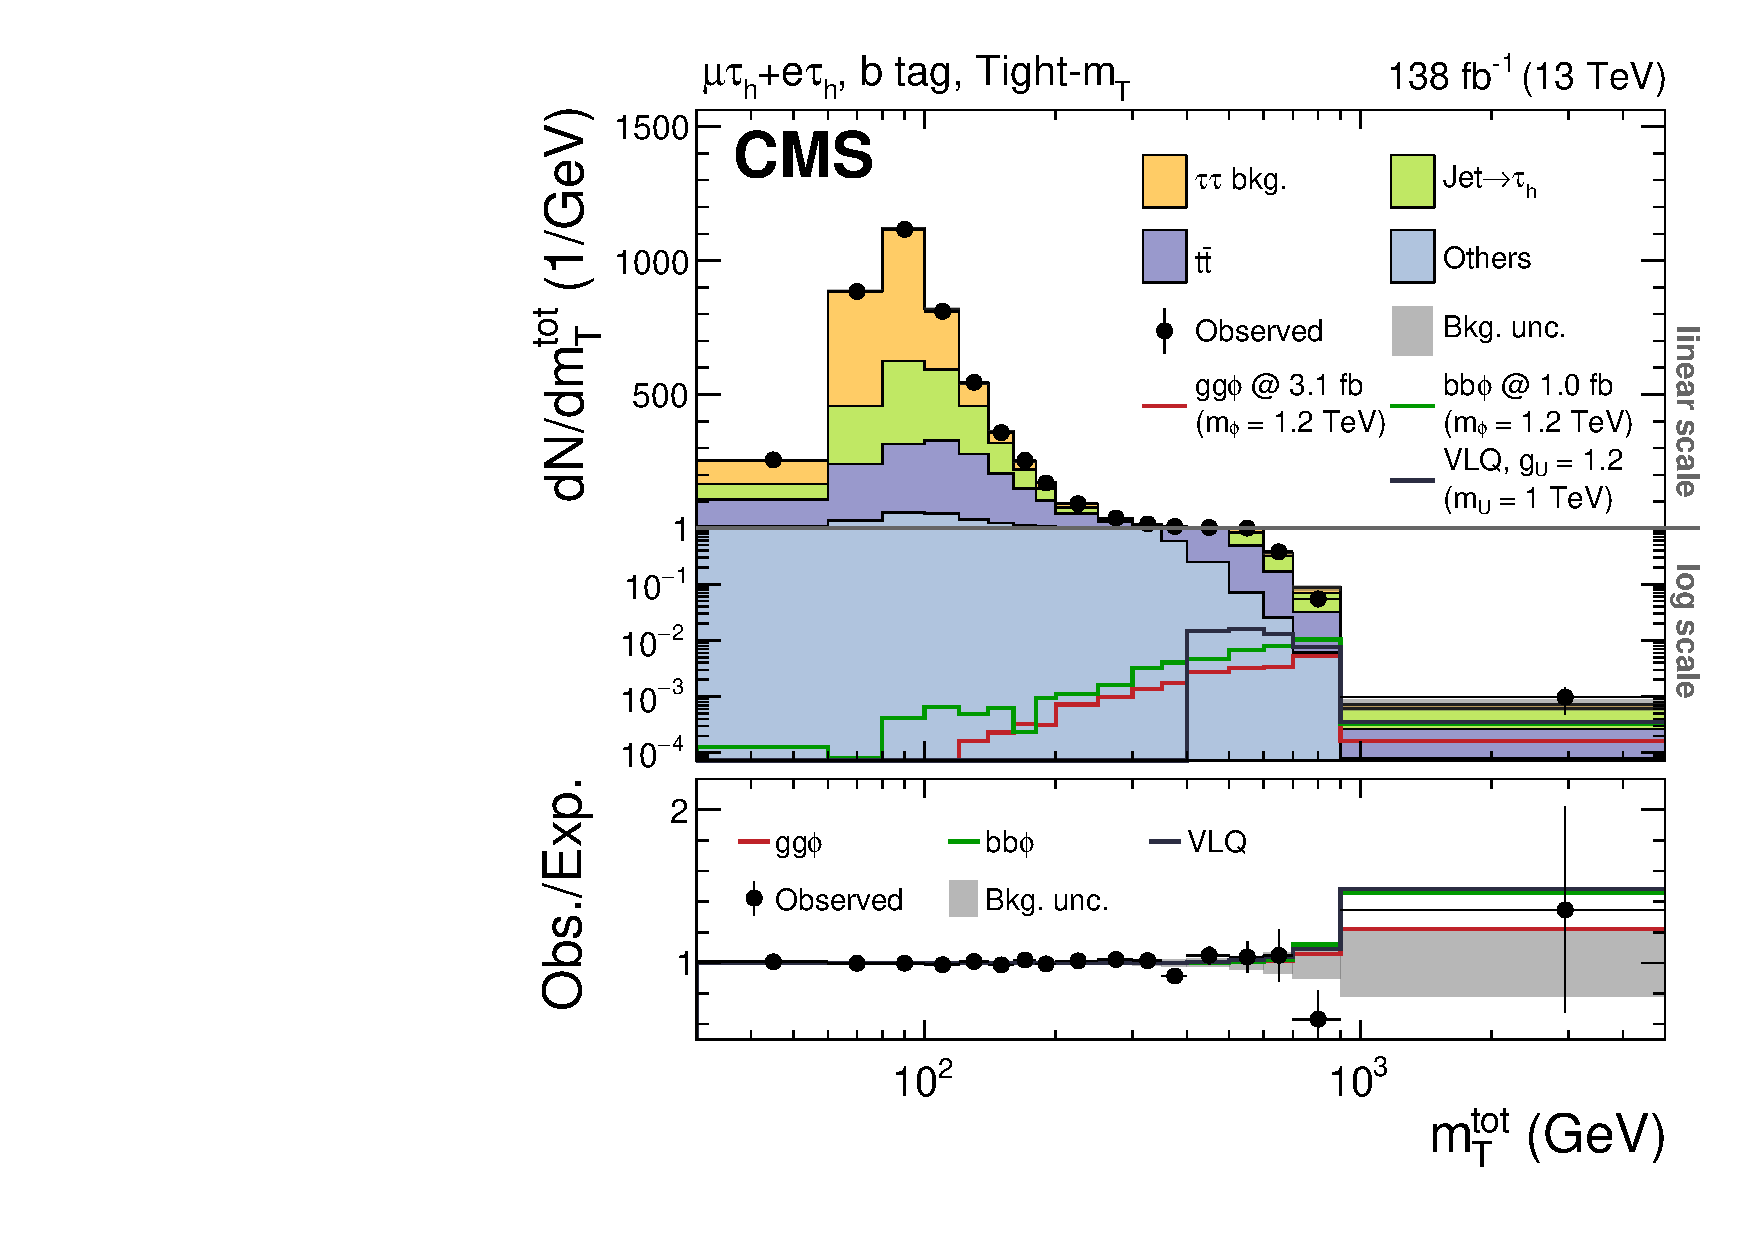
\includegraphics[width=0.45\textwidth]{Figures/postfit_highmass_lt_btag_tightmT.pdf}} \\
    \subfloat[]{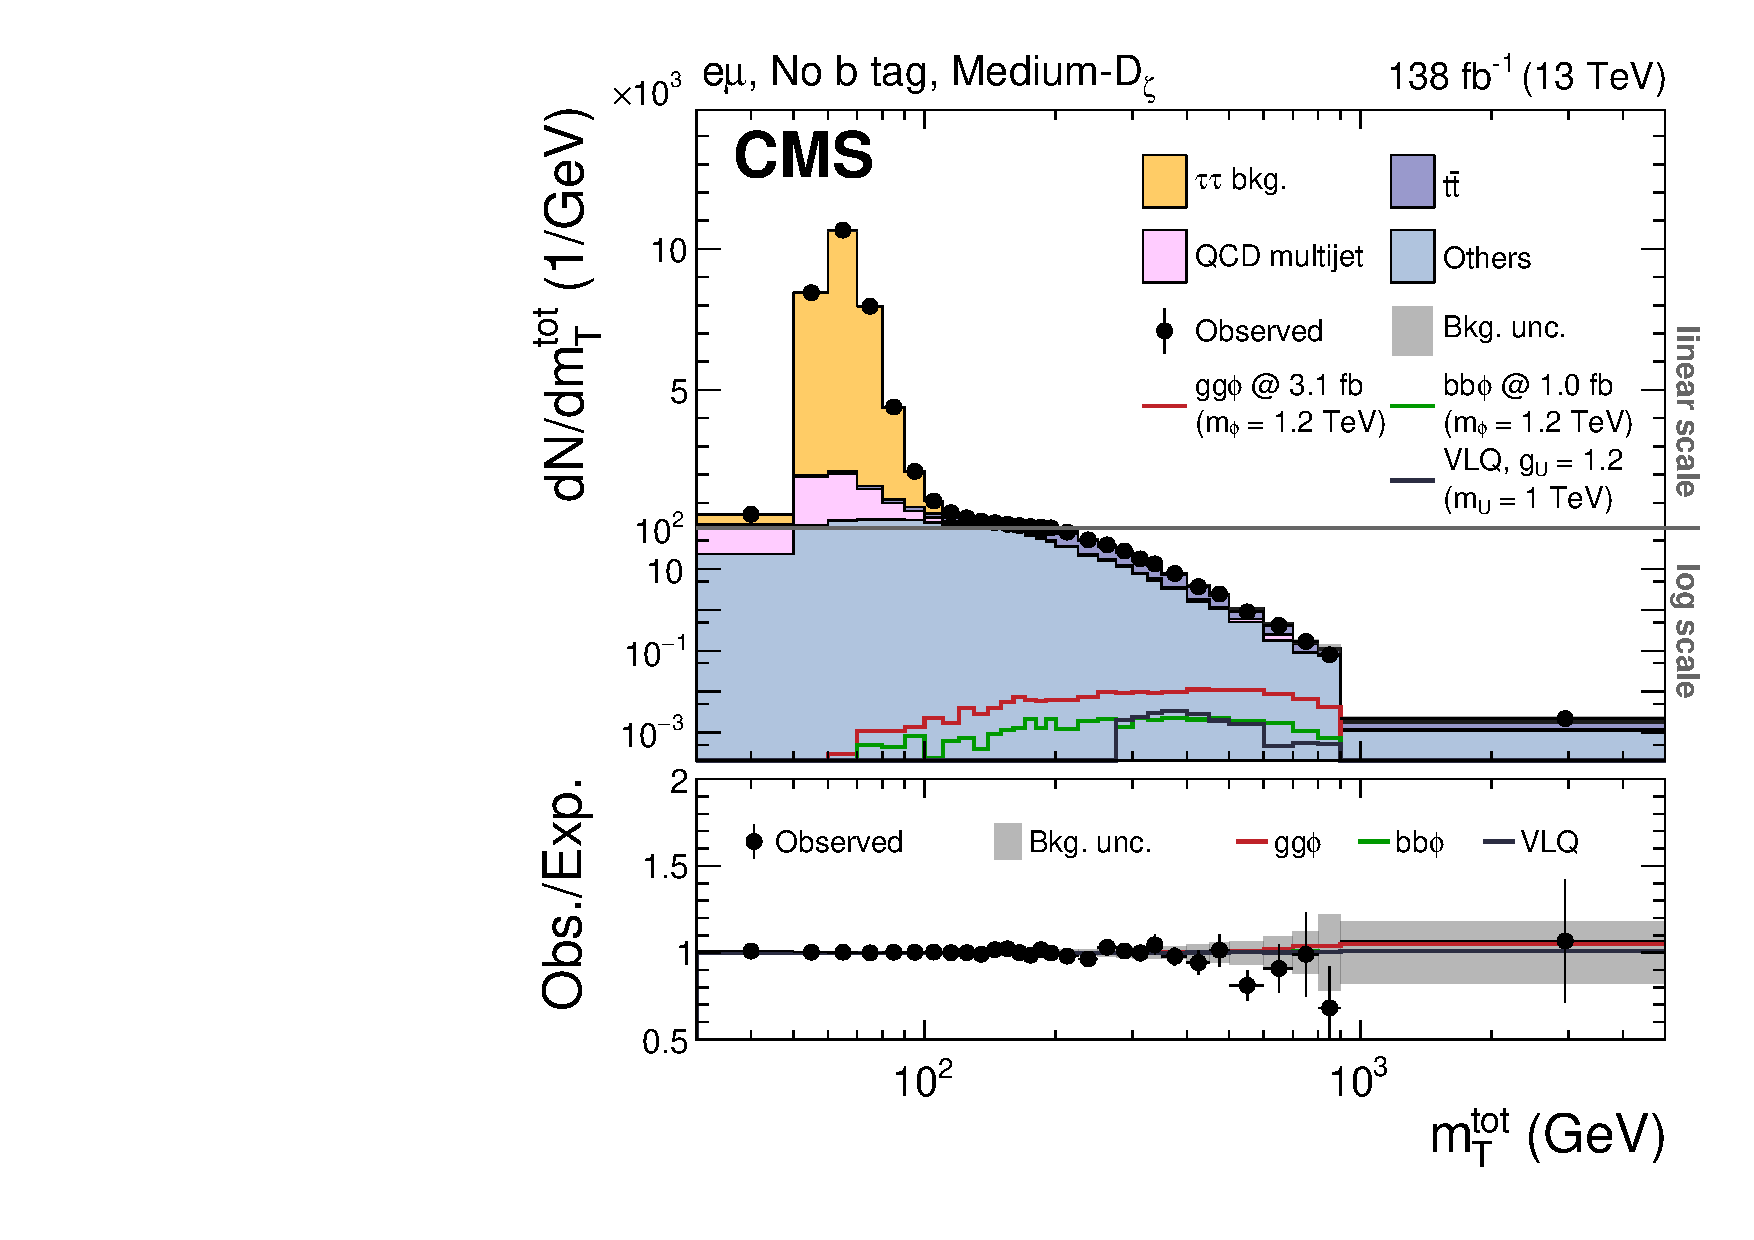
\includegraphics[width=0.45\textwidth]{Figures/postfit_highmass_em_nobtag_mediumdzeta.pdf}}
    \subfloat[]{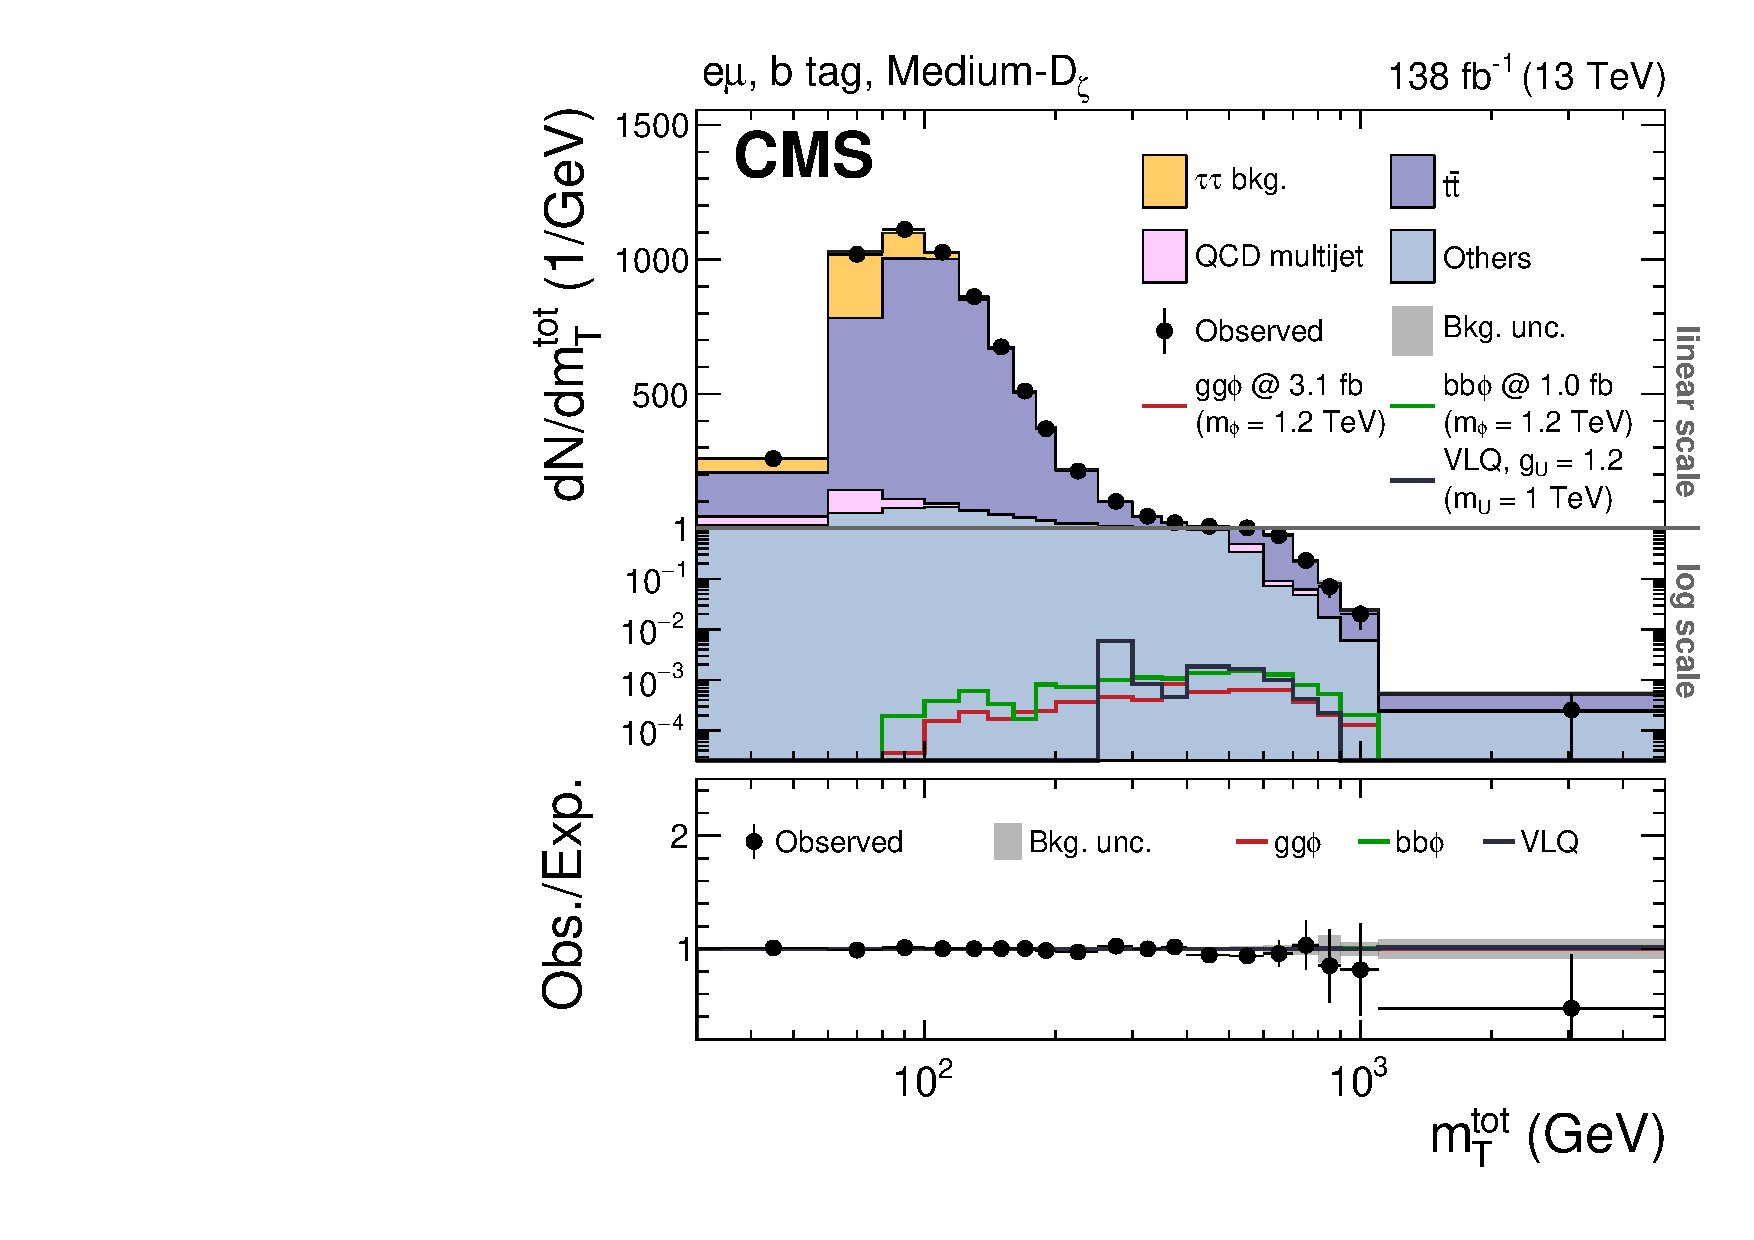
\includegraphics[width=0.45\textwidth]{Figures/postfit_highmass_em_btag_mediumdzeta.pdf}}
\caption{High mass postfit.}
\label{fig:high_mass_postfit}
\end{figure}

\section{MC Corrections}

\section{Model Independent Results}

\subsection{Limit Setting}

\begin{equation}
  q_{\mu} = -2 \ln \Biggl(\frac{\mathcal{L}(\text{data} | \mu, \hat{\theta}_{\mu})}{\mathcal{L}(\text{data} | \hat{\mu}, \hat{\theta}_{\hat{\mu}})}\Biggl), 0 \leq \hat{\mu} \leq \mu,
\end{equation}

\begin{figure}[!hbtp]
\centering
    \subfloat[]{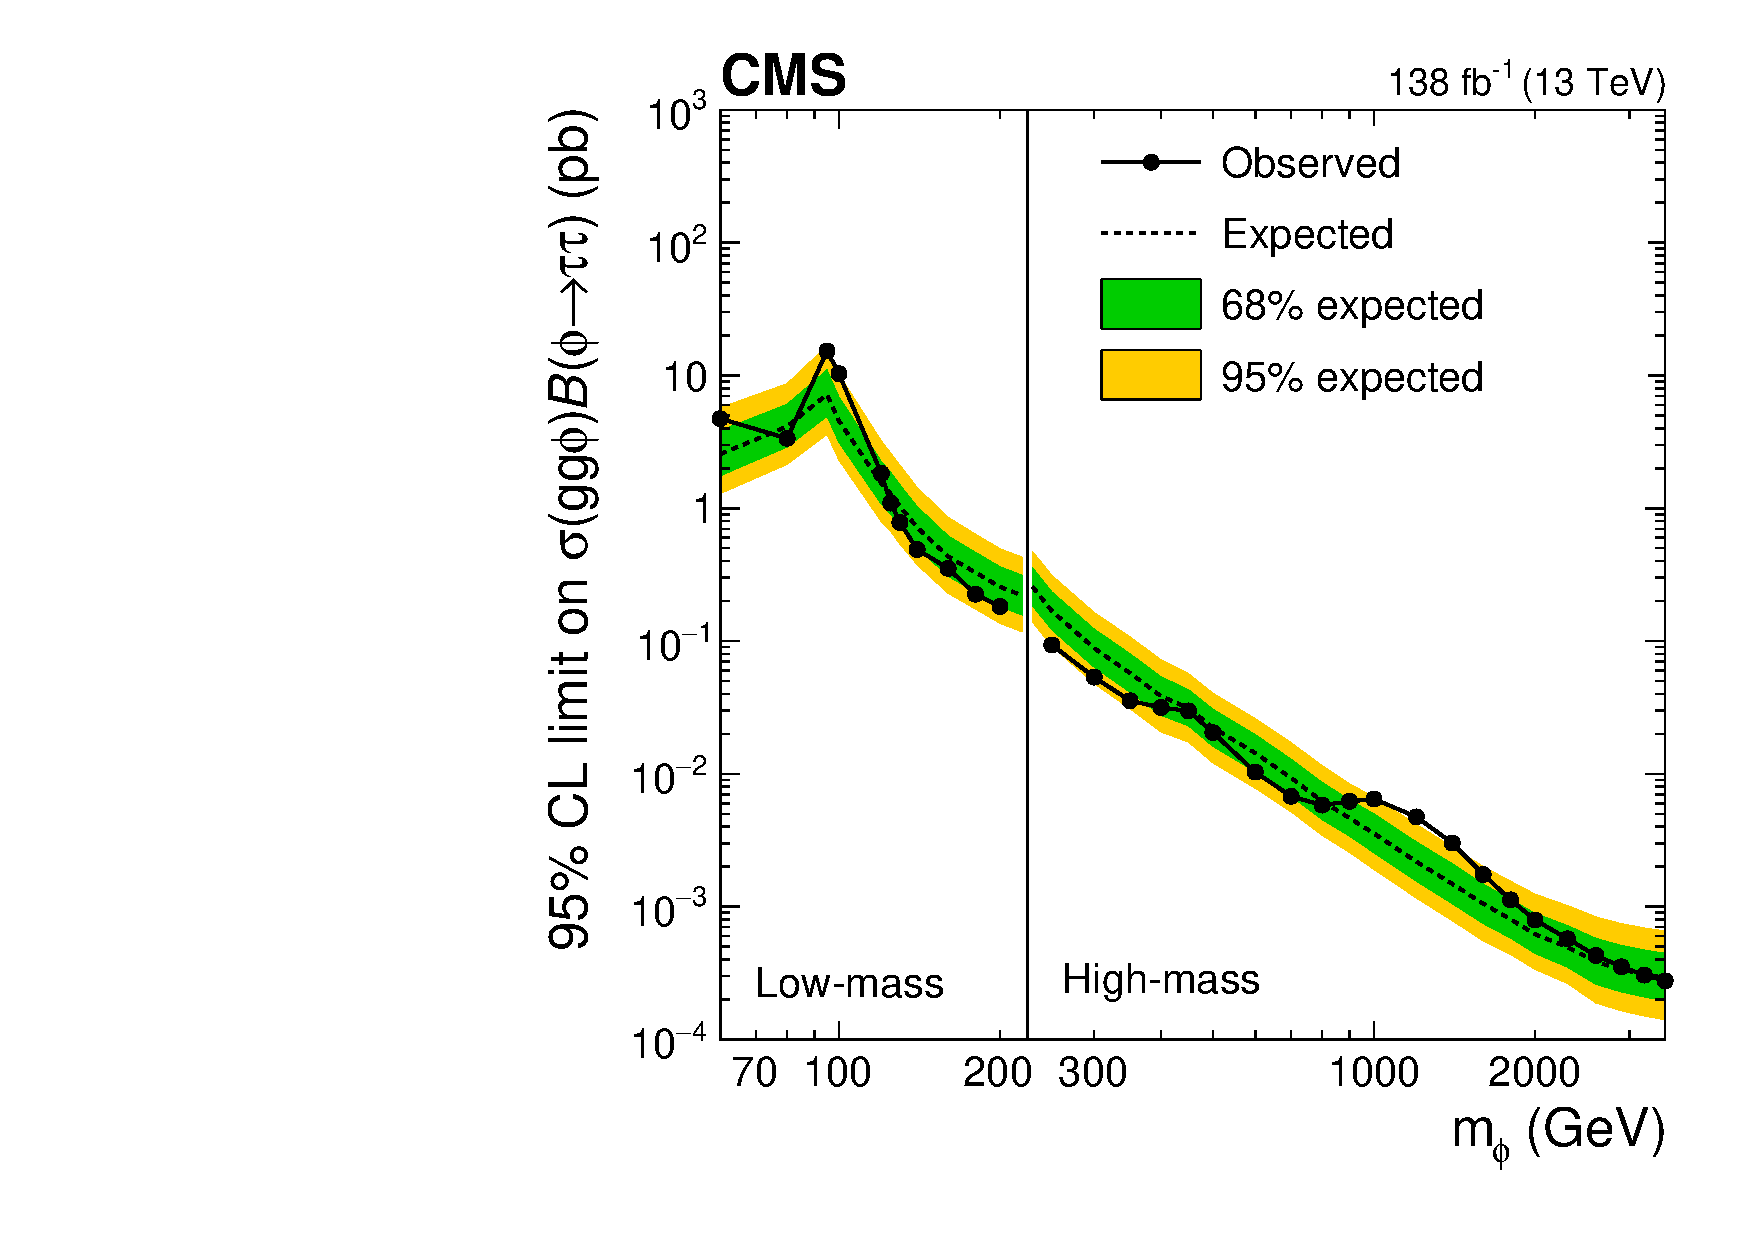
\includegraphics[width=0.5\textwidth]{Figures/model_independent_limit_ggH.pdf}}
    \subfloat[]{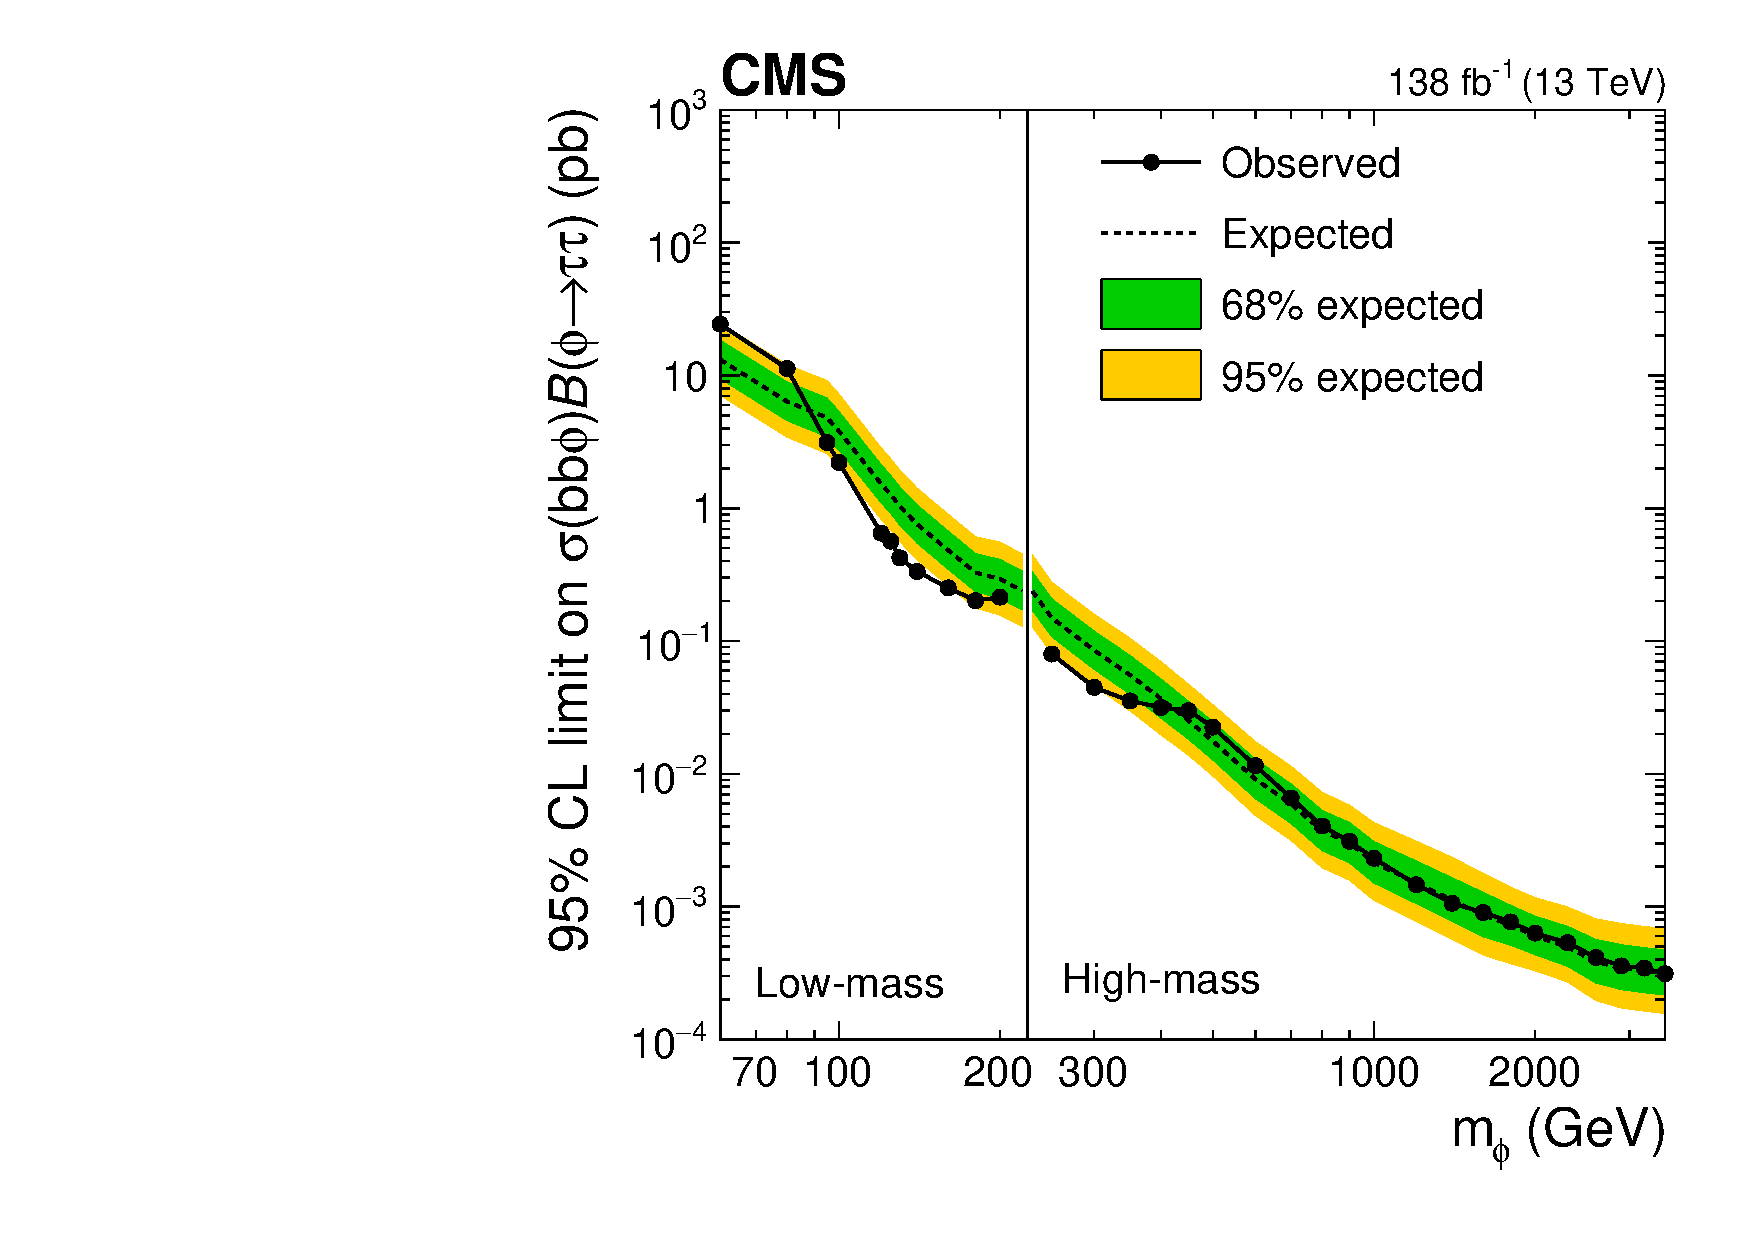
\includegraphics[width=0.5\textwidth]{Figures/model_independent_limit_bbH.pdf}}
\caption{Model independent limits.}
\label{fig:model_independent_limits}
\end{figure}

\begin{figure}[!hbtp]
\centering
    \subfloat[]{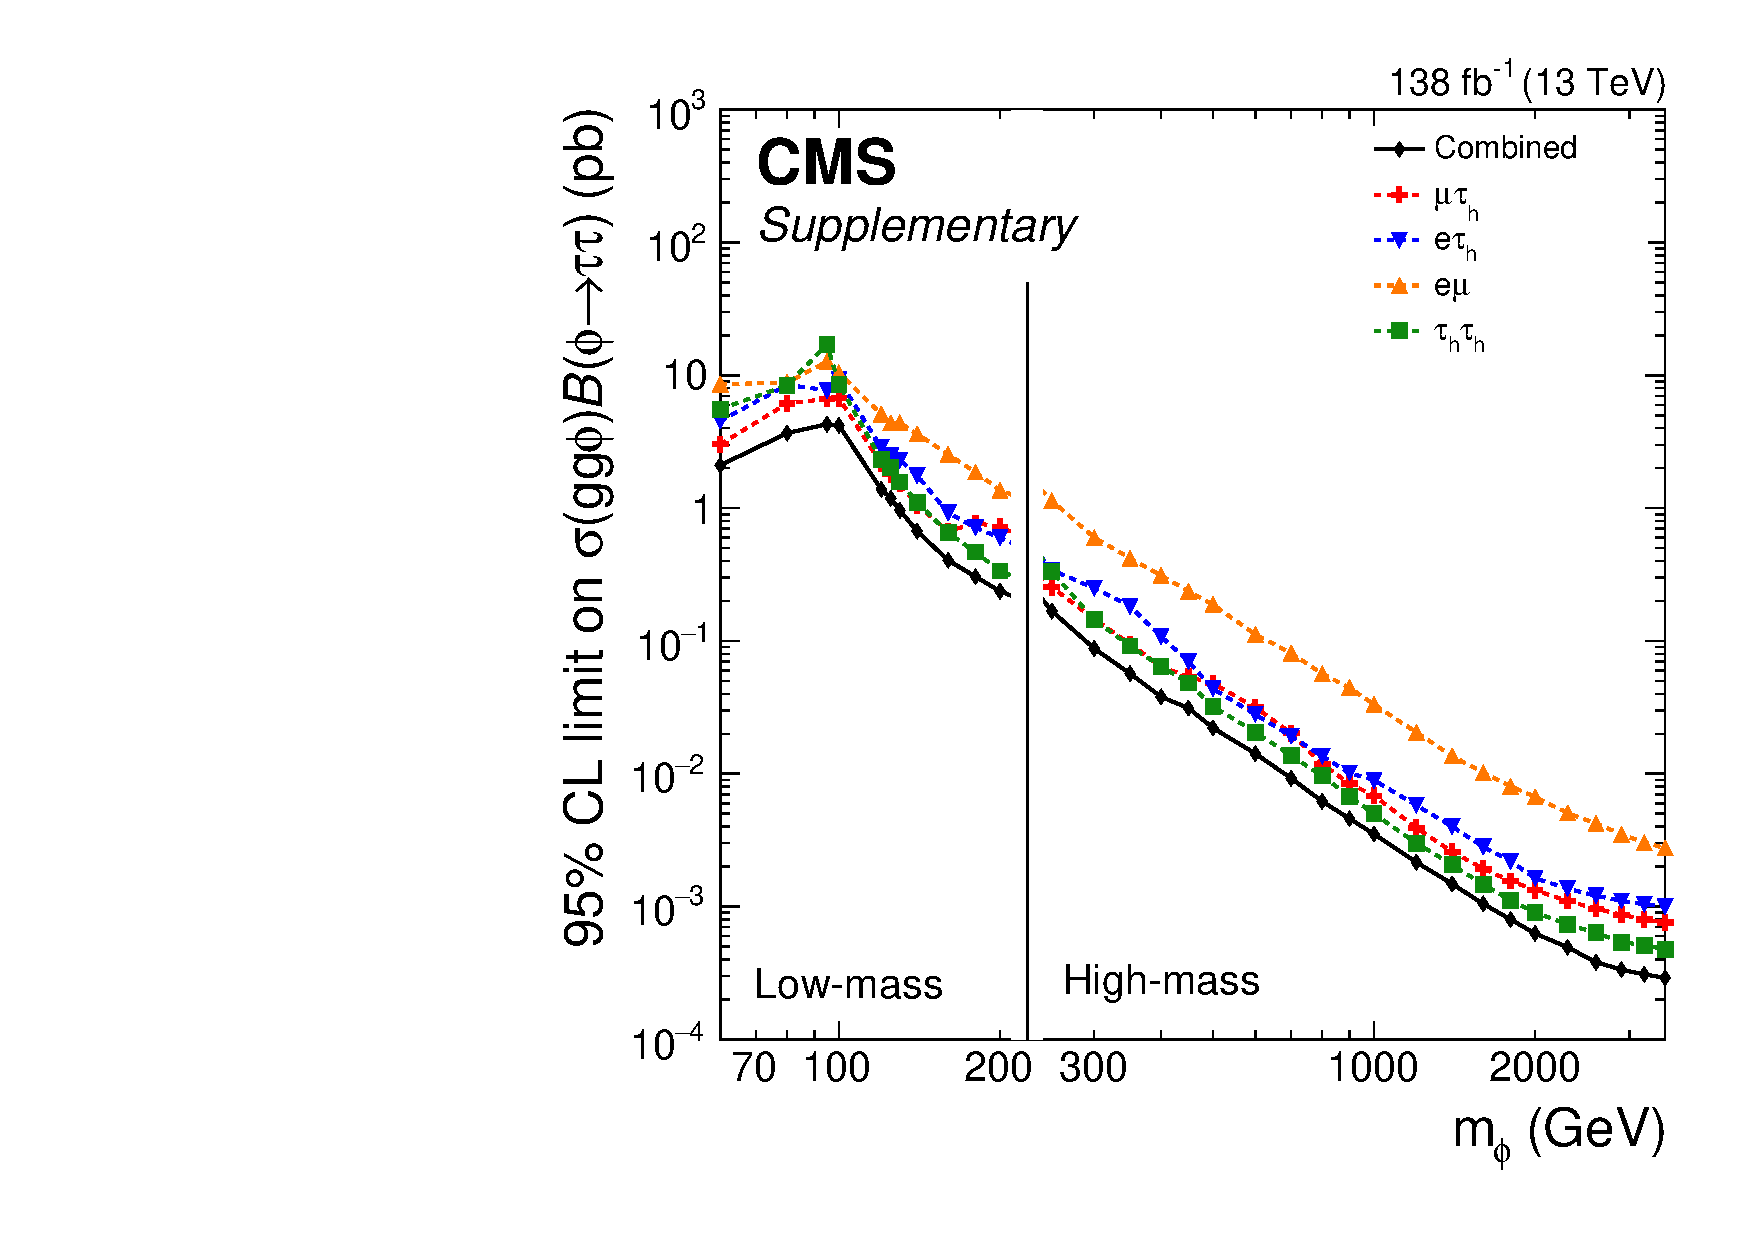
\includegraphics[width=0.5\textwidth]{Figures/limit_comparison_mssm_ggphi.pdf}}
    \subfloat[]{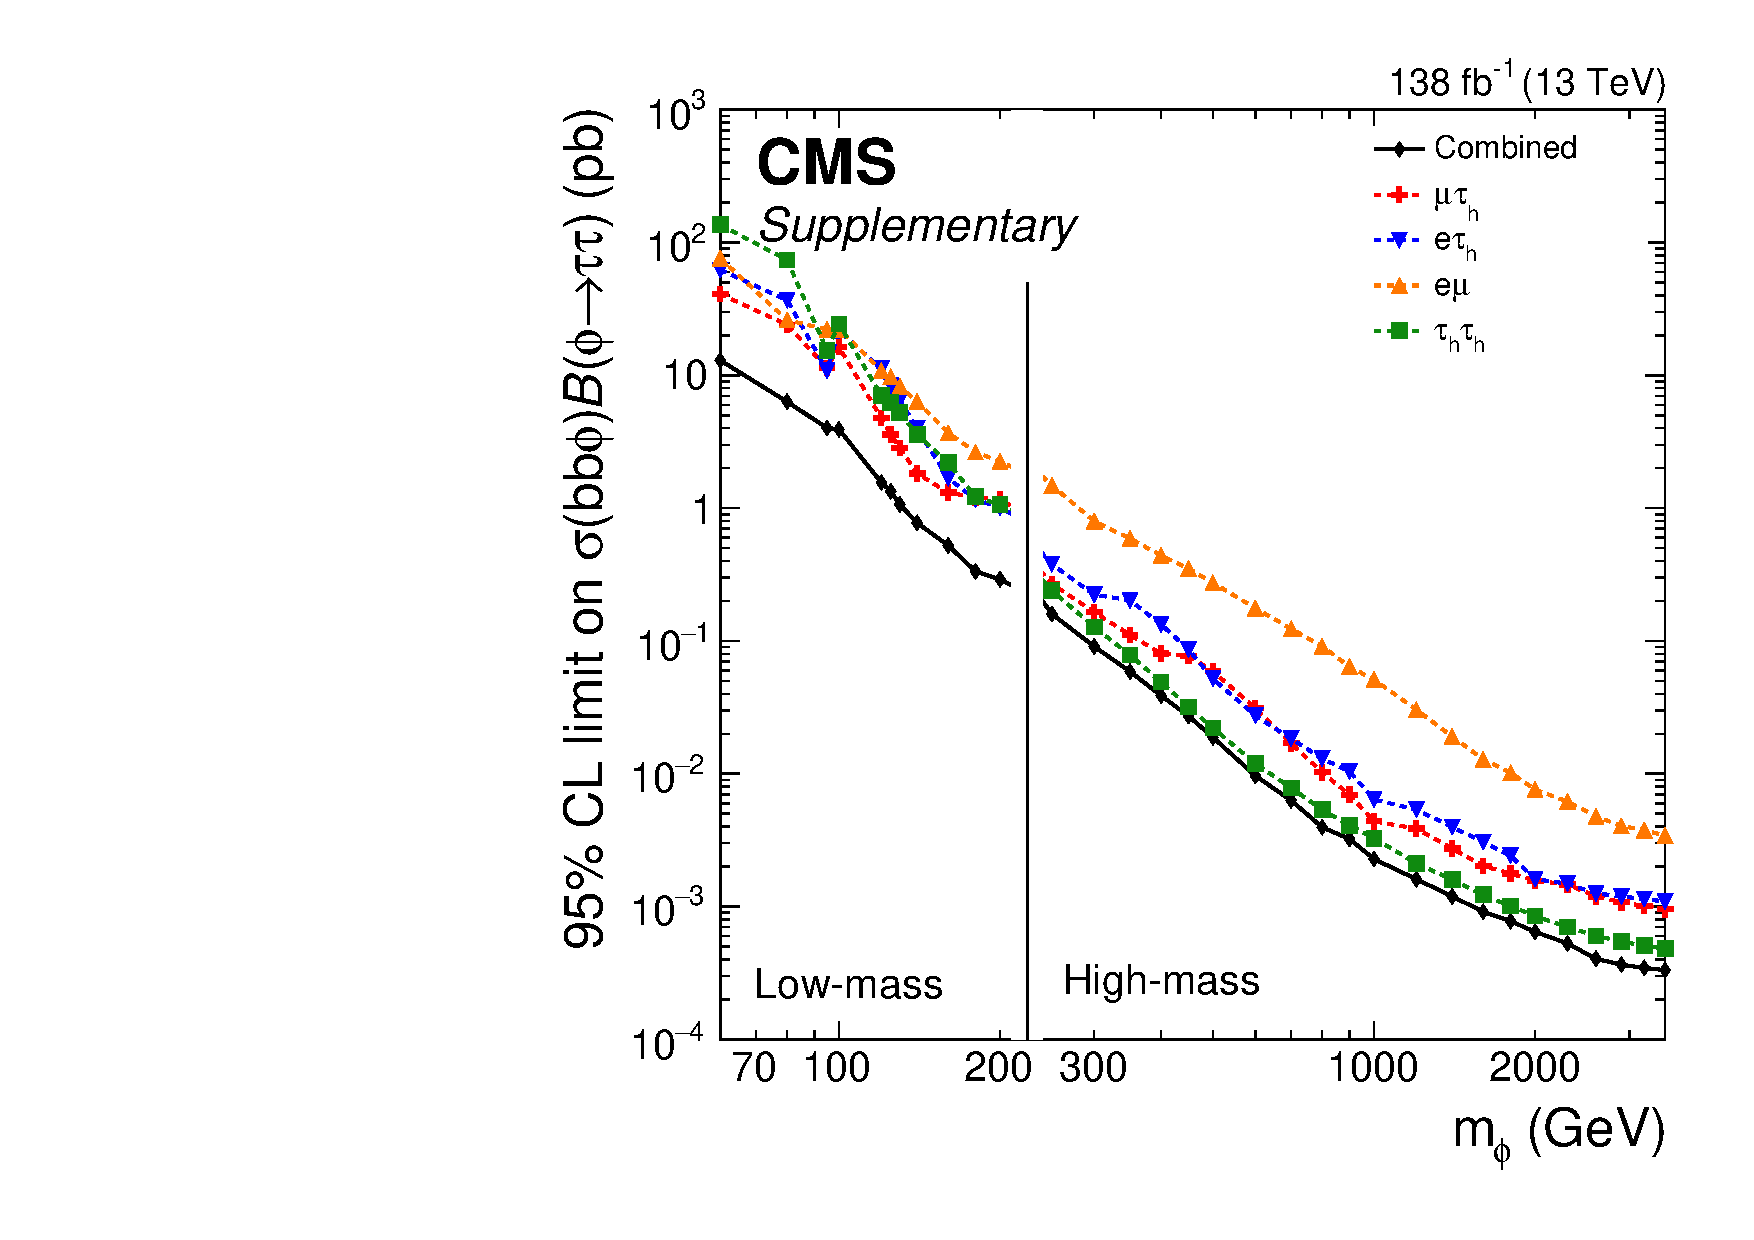
\includegraphics[width=0.5\textwidth]{Figures/limit_comparison_mssm_bbphi.pdf}}
\caption{Model independent limits.}
\label{fig:model_independent_limits_by_channel}
\end{figure}

\begin{figure}[!hbtp]
\centering
    \subfloat[]{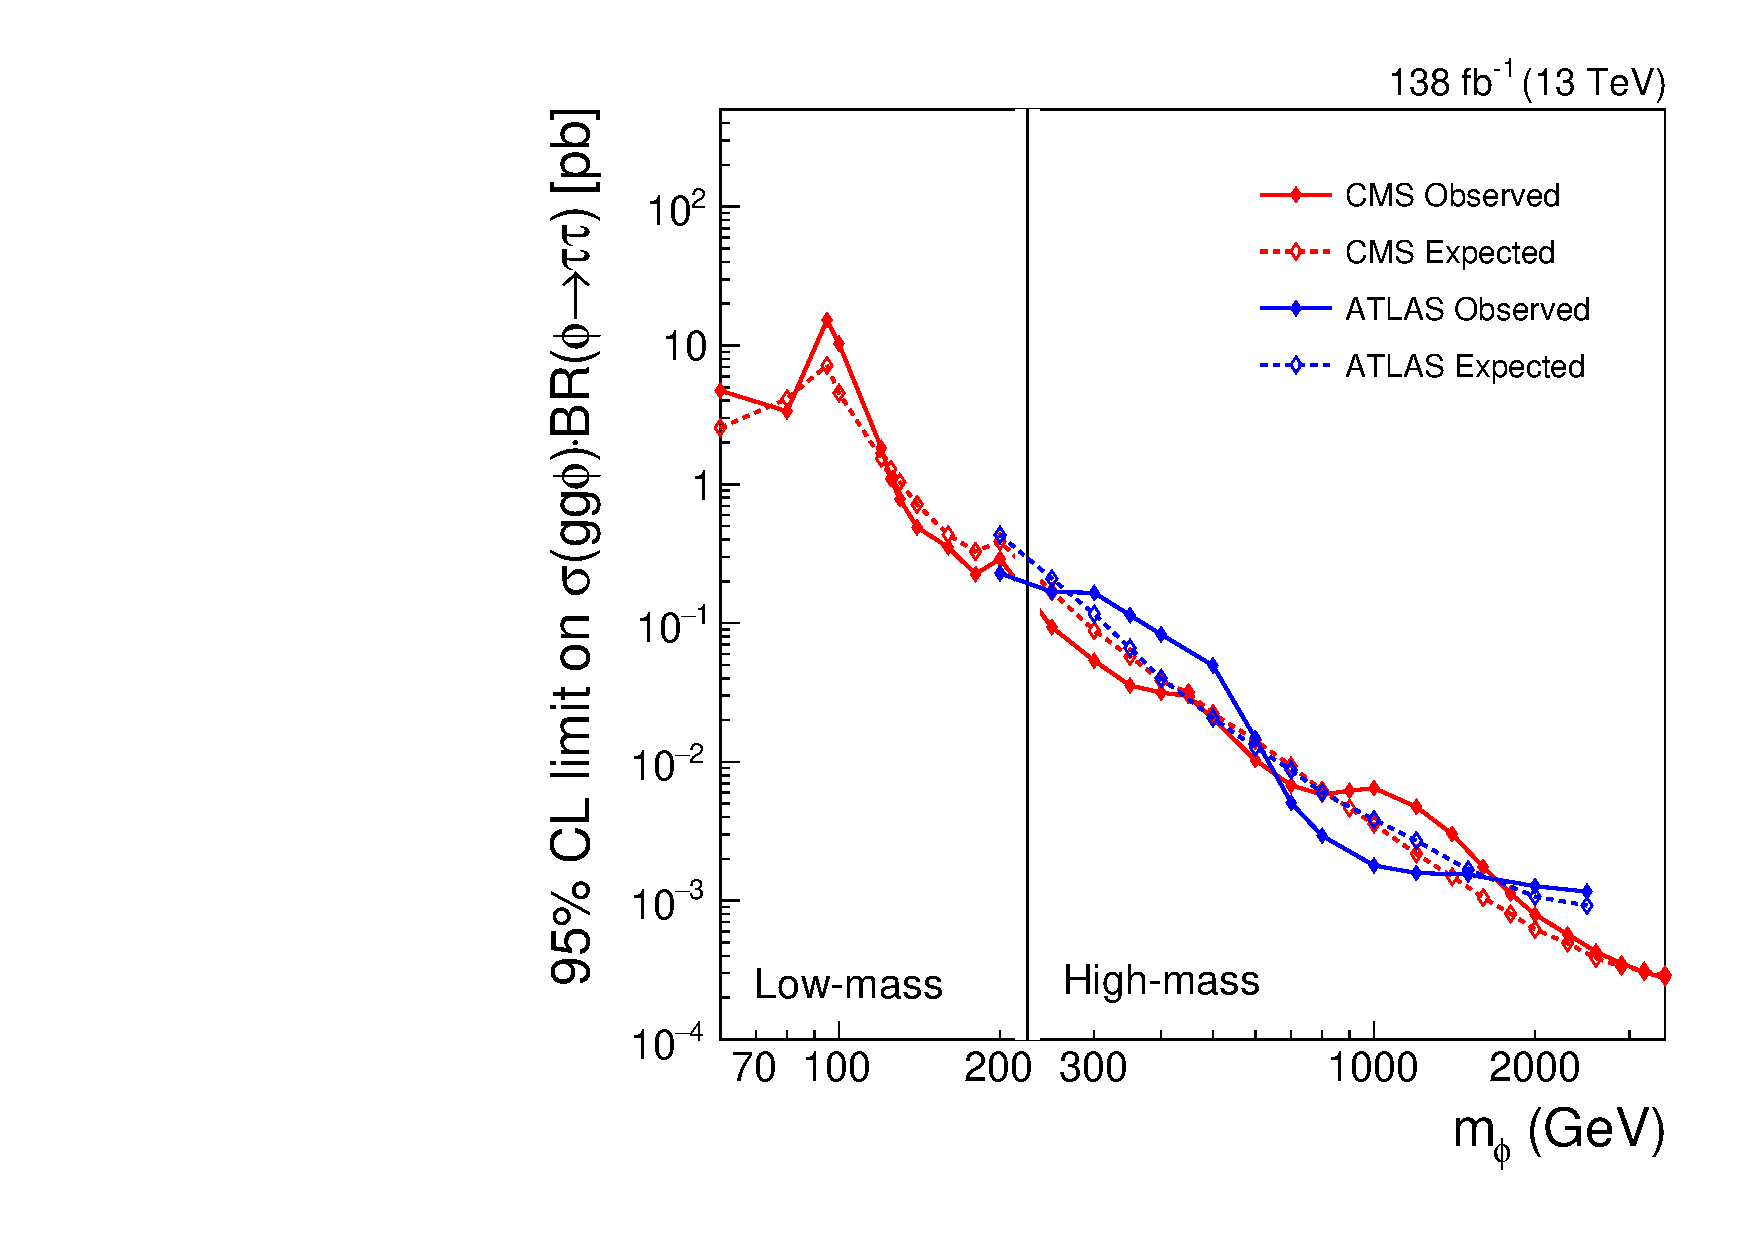
\includegraphics[width=0.5\textwidth]{Figures/limit_comparison_gg_ATLAS.pdf}}
    \subfloat[]{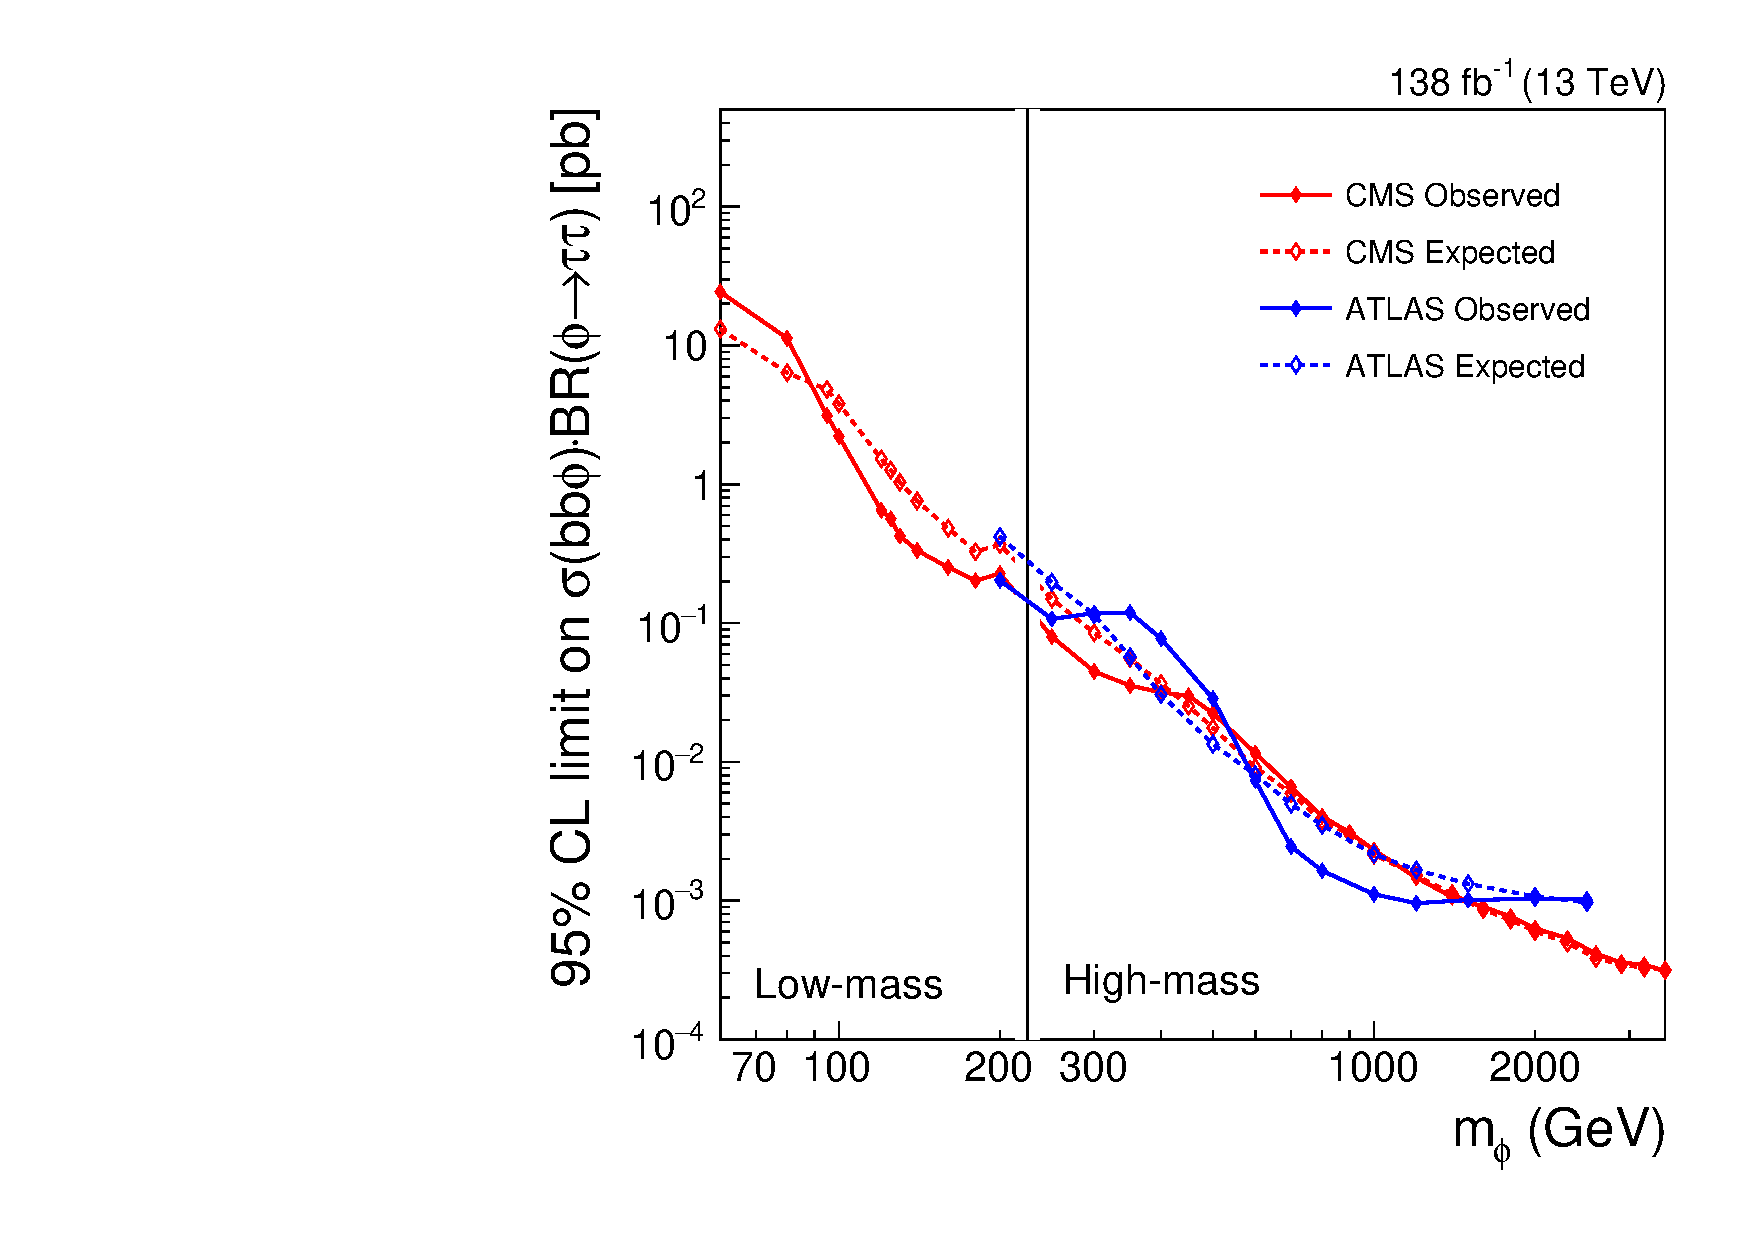
\includegraphics[width=0.5\textwidth]{Figures/limit_comparison_bb_ATLAS.pdf}}
\caption{Model independent limits.}
\label{fig:model_independent_limits_by_channel}
\end{figure}

\subsection{Significance and Compatibility}

\begin{figure}[!hbtp]
\centering
    \subfloat[]{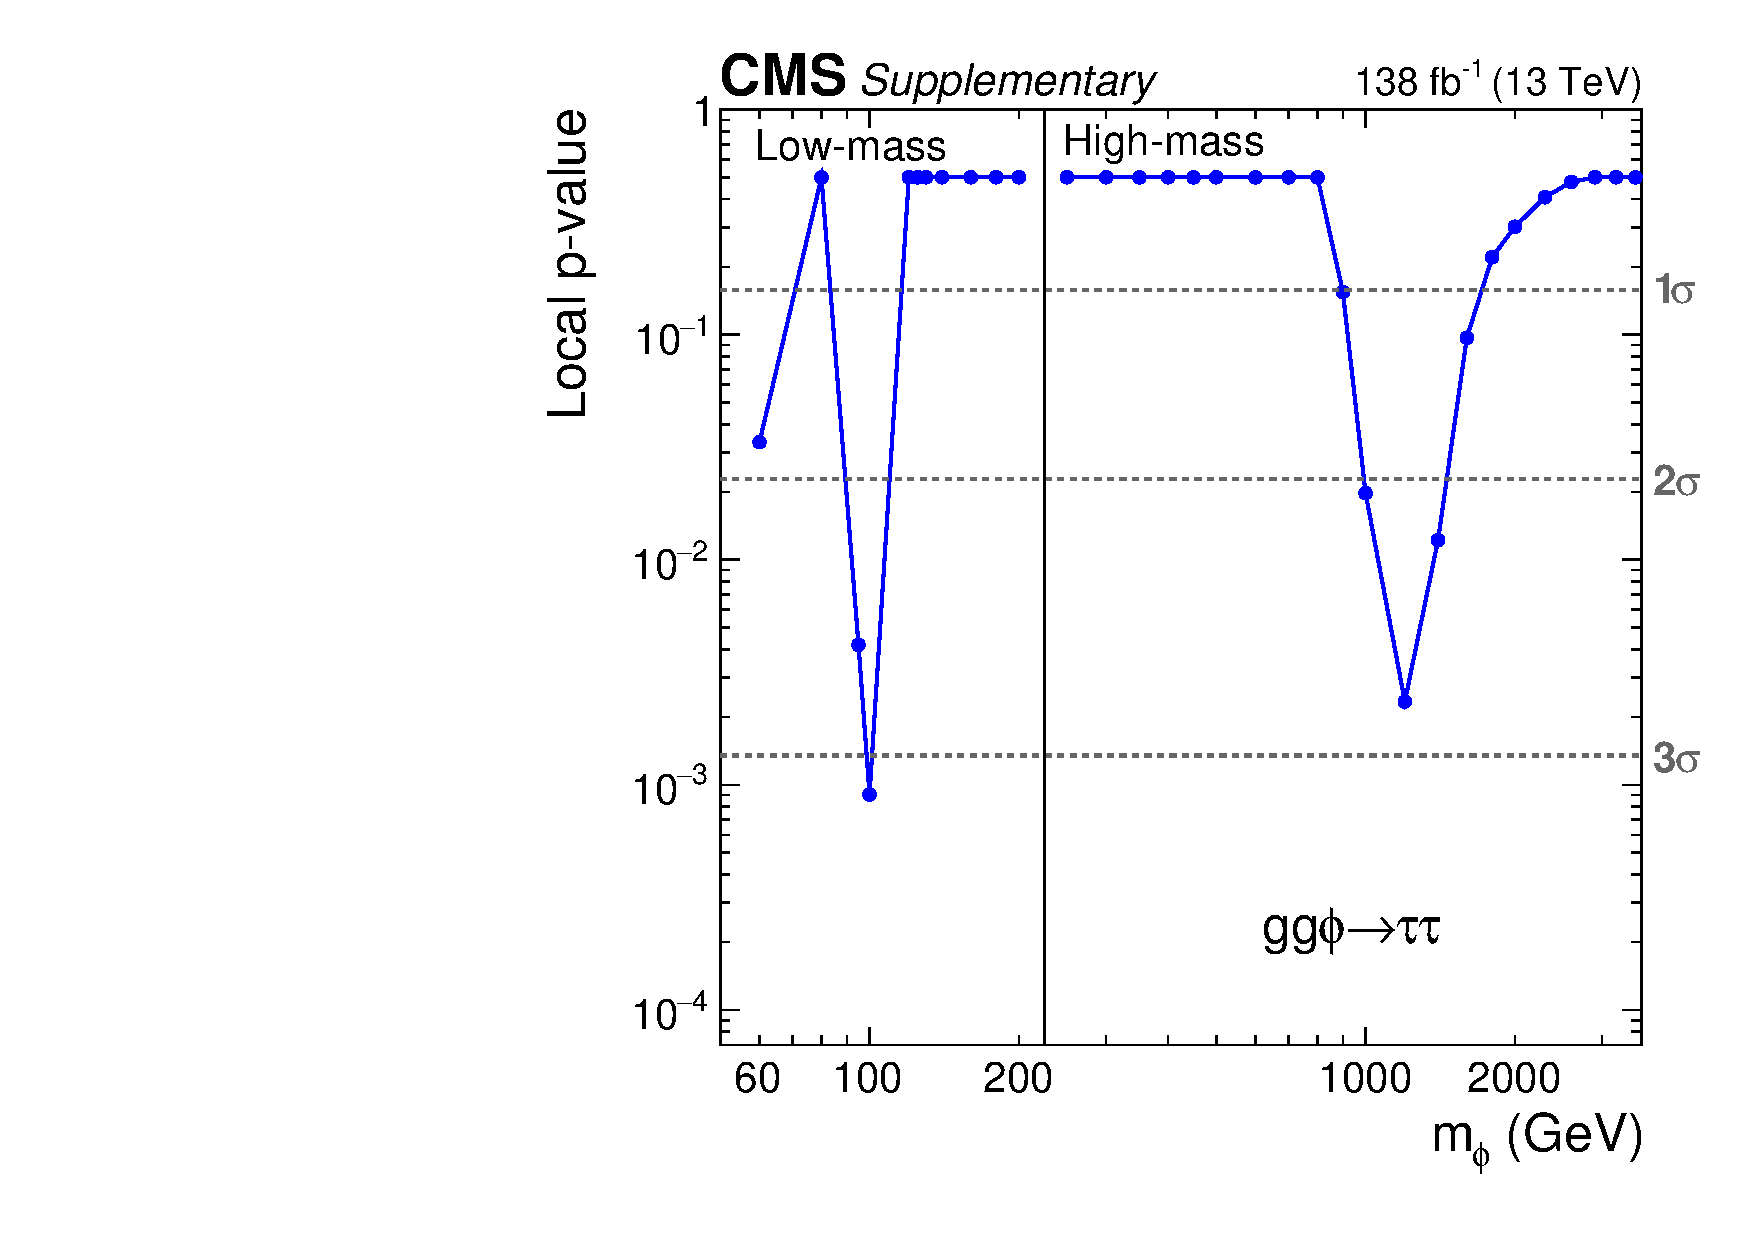
\includegraphics[width=0.5\textwidth]{Figures/significance_plot_ggH.pdf}}
    \subfloat[]{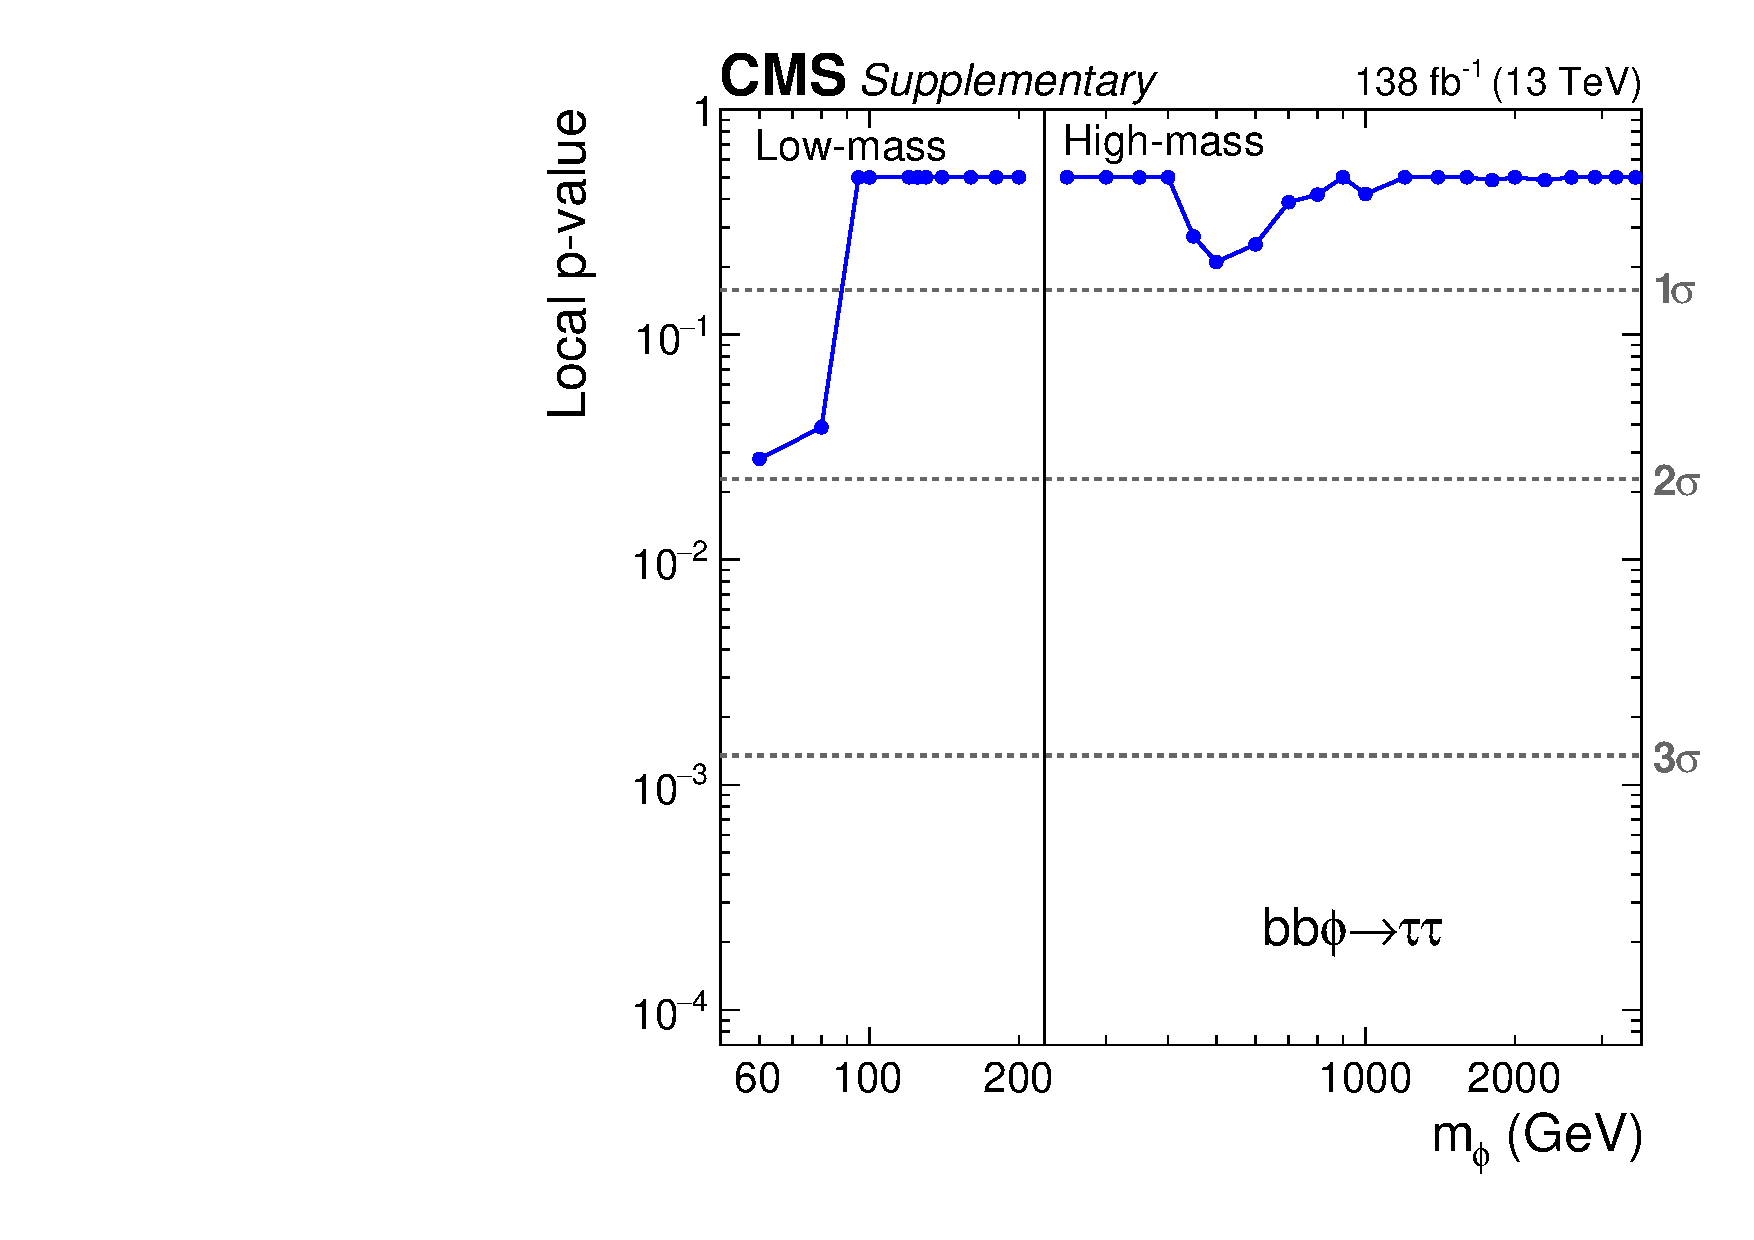
\includegraphics[width=0.5\textwidth]{Figures/significance_plot_bbH.pdf}}
\caption{Significance.}
\label{fig:significance}
\end{figure}

\begin{figure}[!hbtp]
\centering
    \subfloat[]{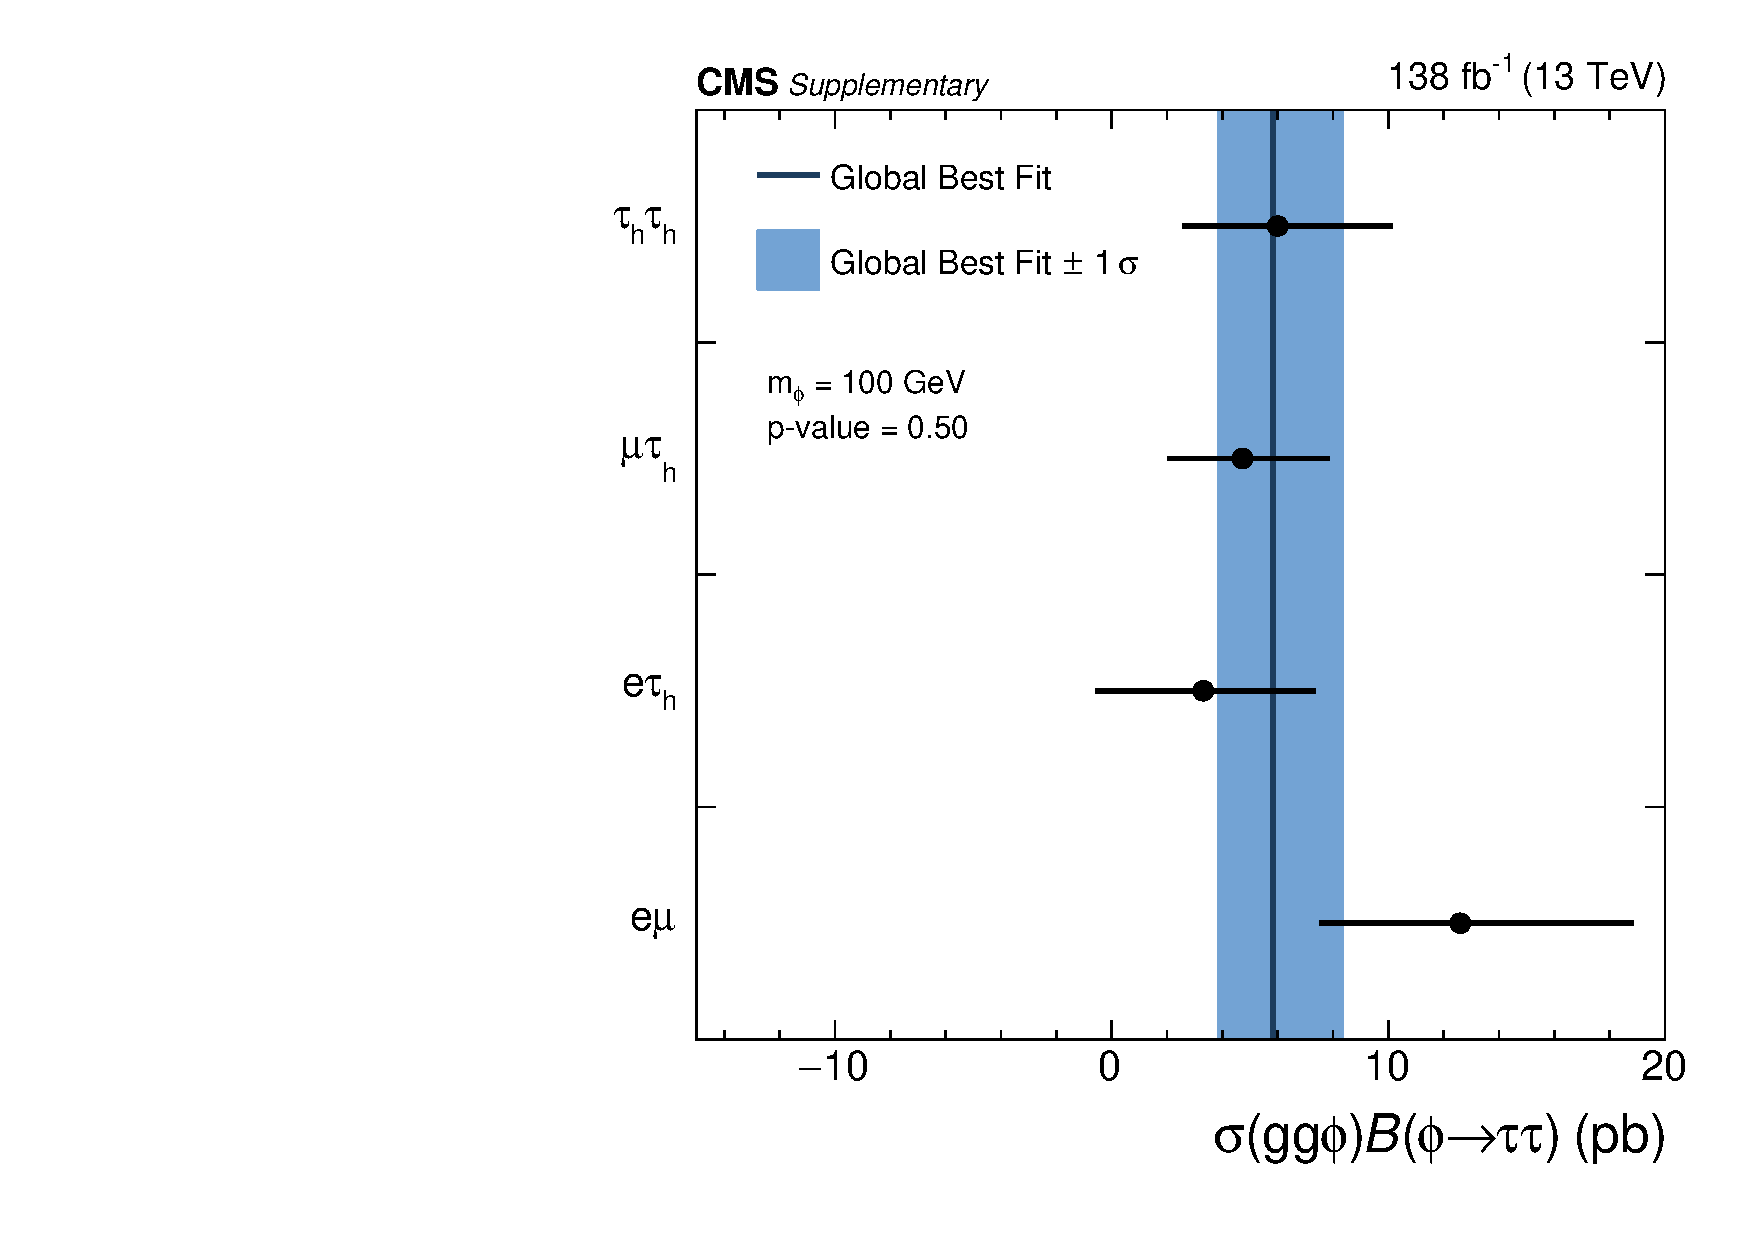
\includegraphics[width=0.5\textwidth]{Figures/ChannelCompatibilityCheck_FitResults_mH100_channel.pdf}}
    \subfloat[]{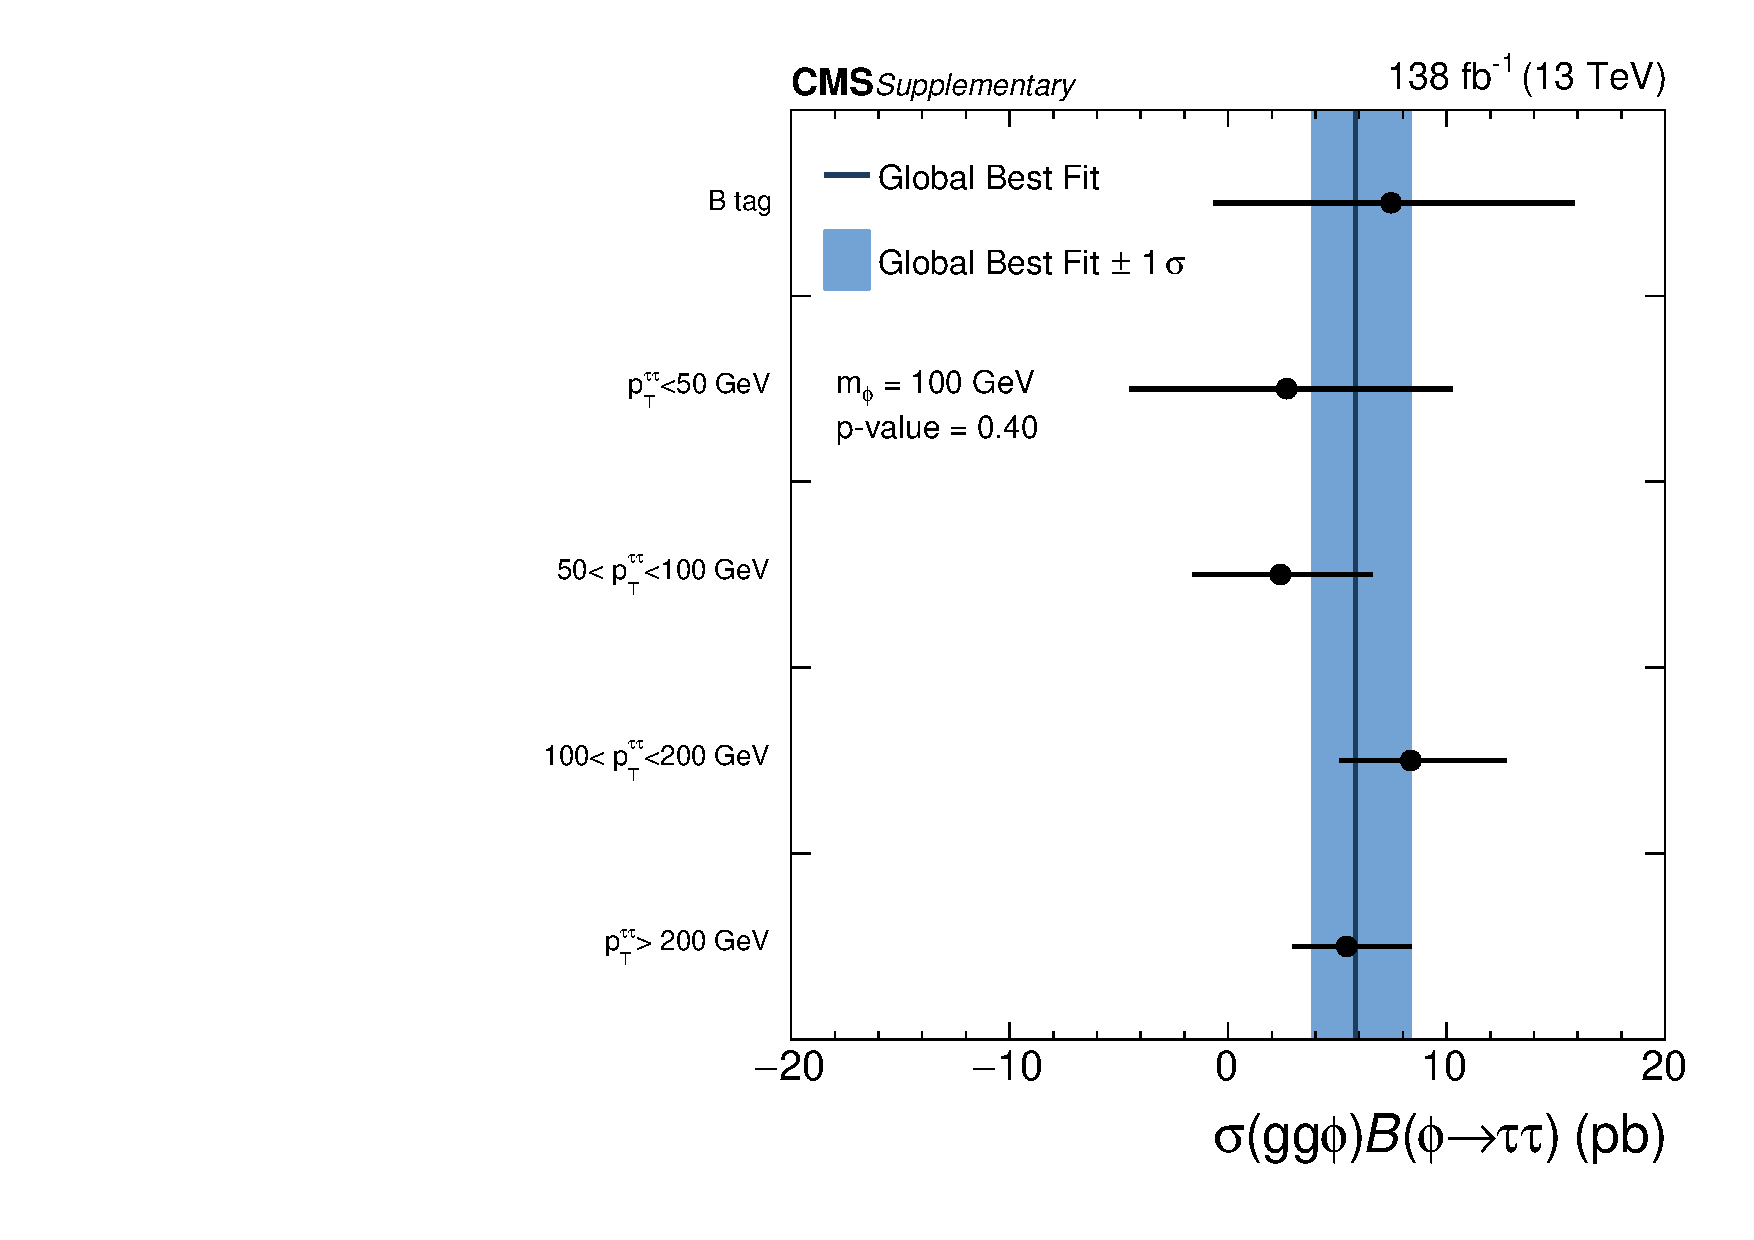
\includegraphics[width=0.5\textwidth]{Figures/ChannelCompatibilityCheck_FitResults_mH100_cat.pdf}}
\caption{Low mass compatibility.}
\label{fig:low_mass_compatibility}
\end{figure}

\begin{figure}[!hbtp]
\centering
    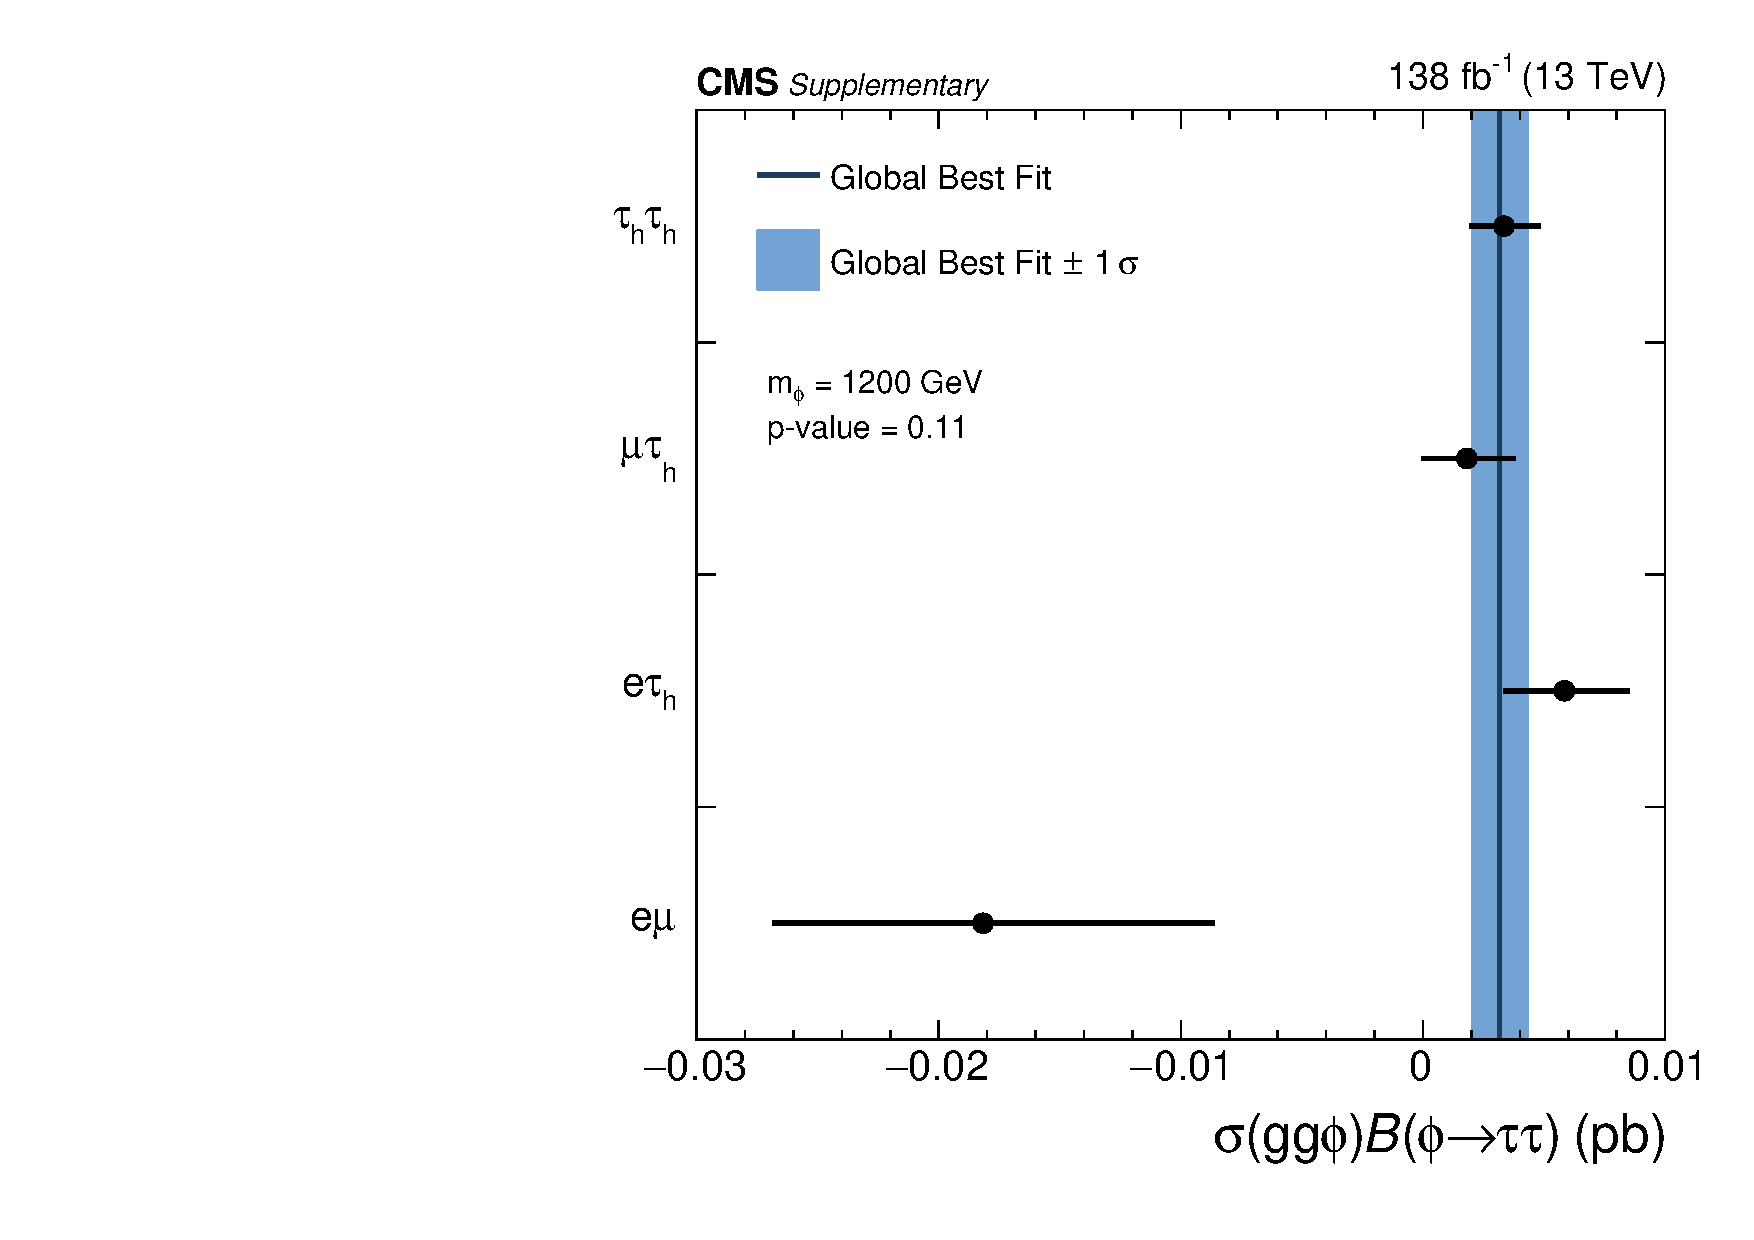
\includegraphics[width=0.5\textwidth]{Figures/ccc_fit_result_mH1200_per-channel.pdf}
\caption{High mass compatibility.}
\label{fig:high_mass_compatibility}
\end{figure}

\subsection{2D Likelihood Scans}

\begin{figure}[!hbtp]
\centering
    \subfloat[]{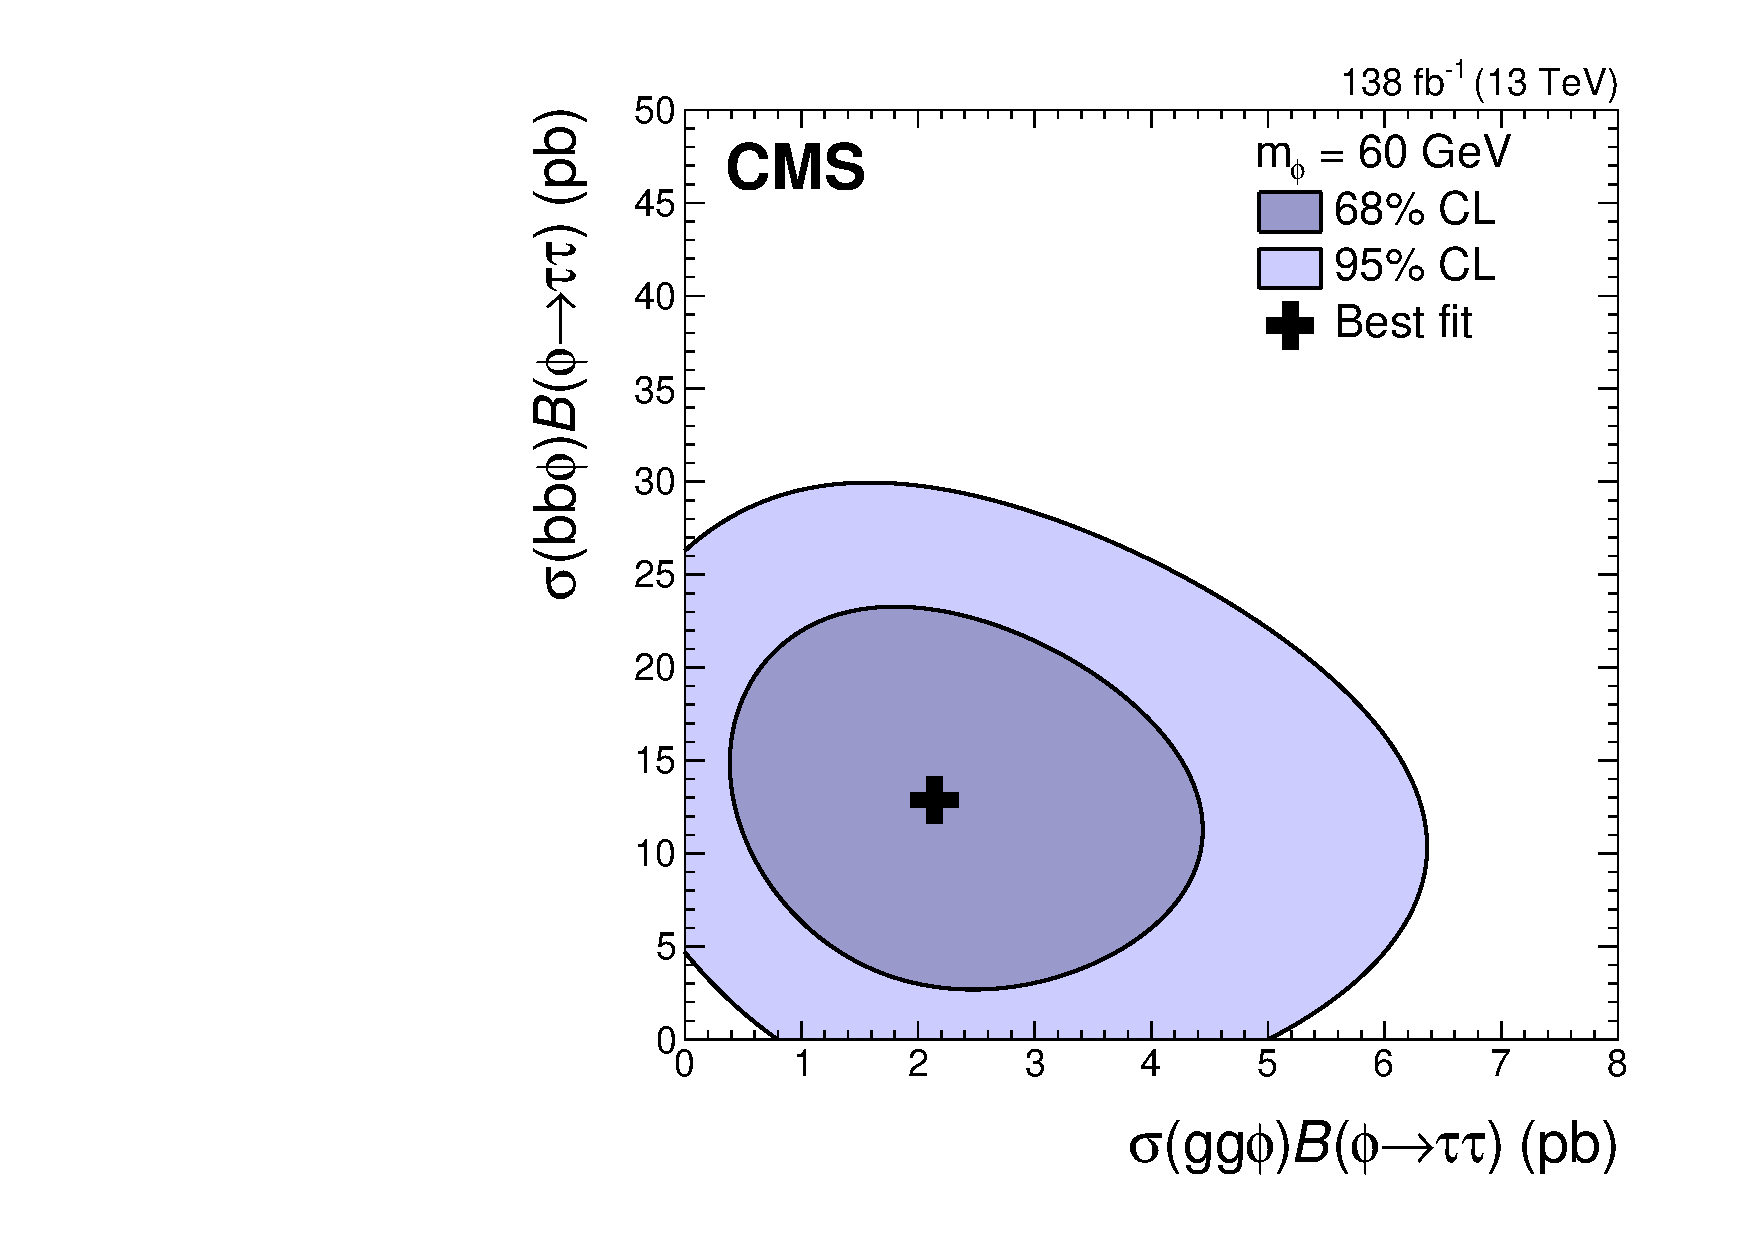
\includegraphics[width=0.33\textwidth]{Figures/2d_lkld_60.pdf}}
    \subfloat[]{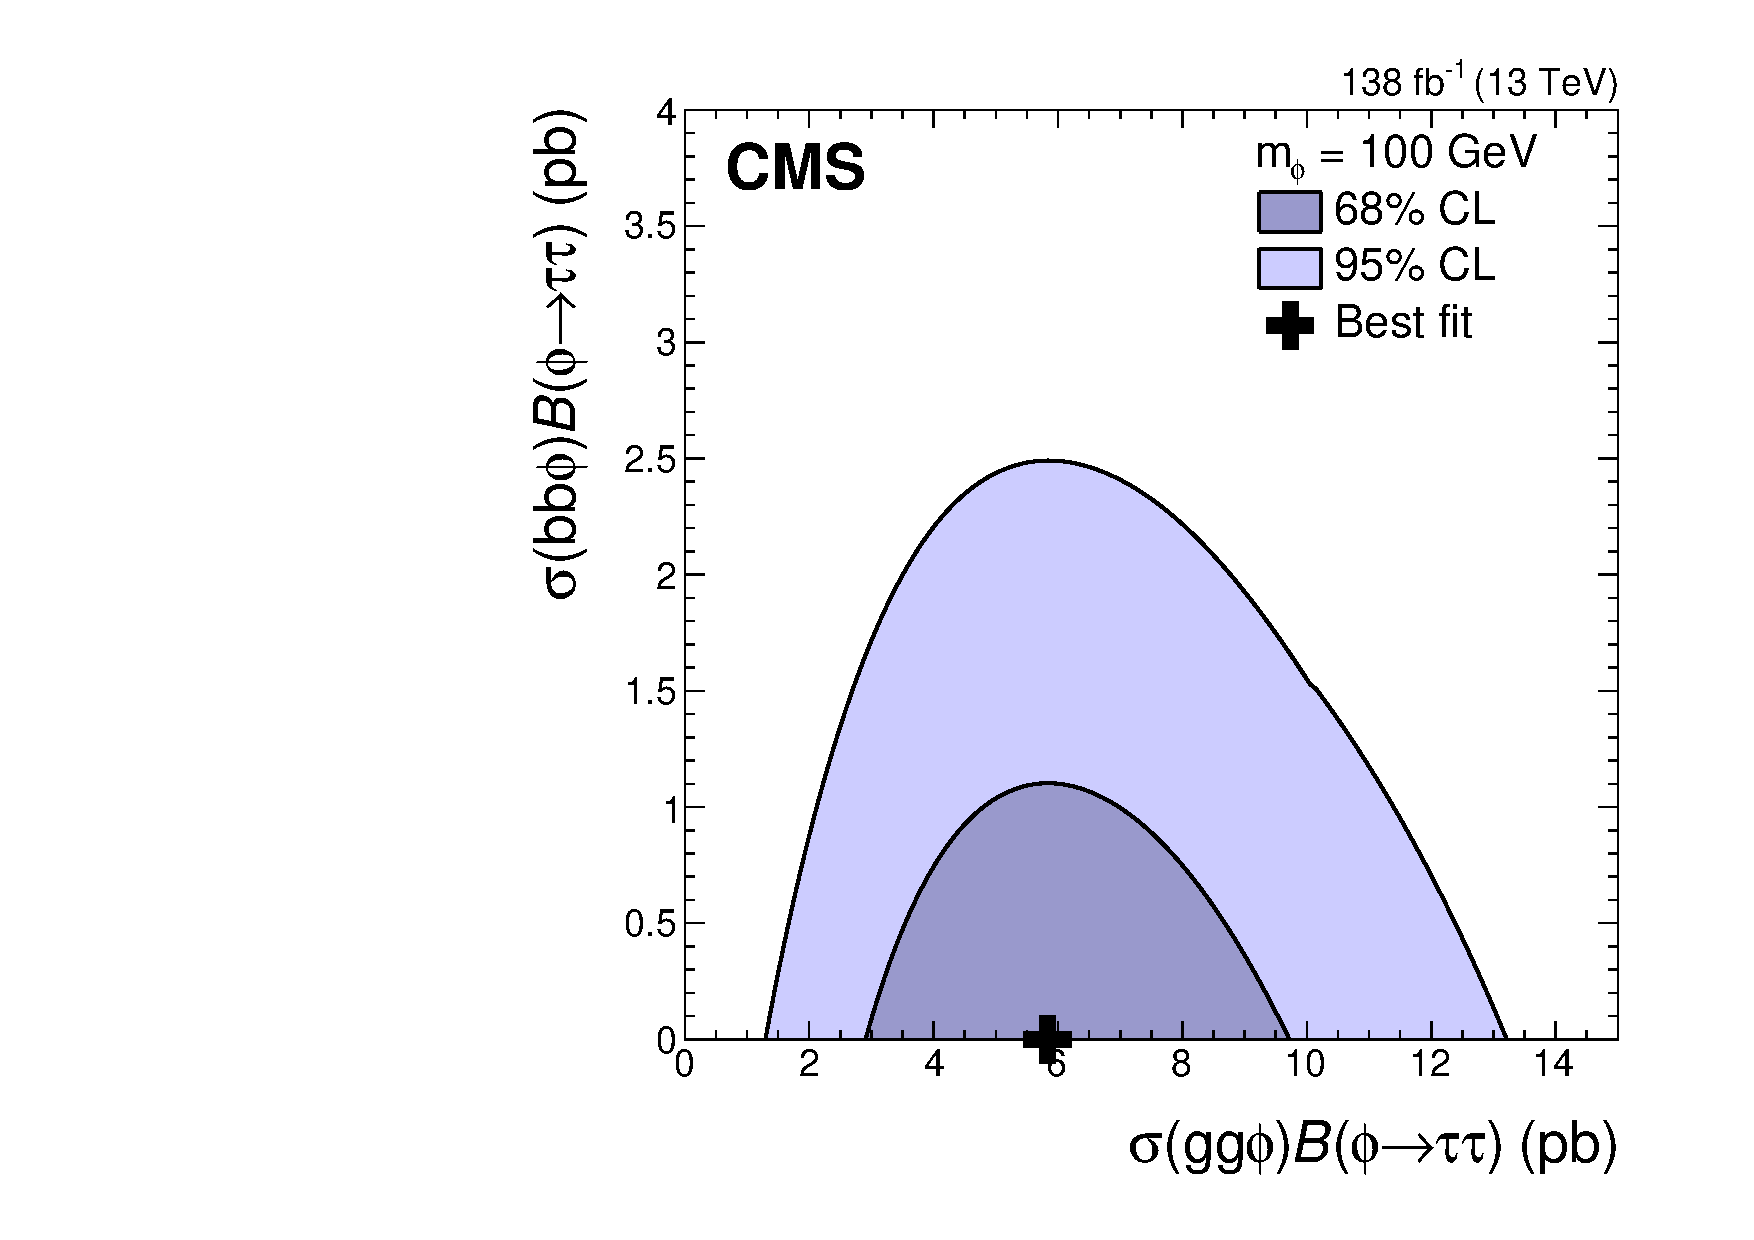
\includegraphics[width=0.33\textwidth]{Figures/2d_lkld_100.pdf}}
    \subfloat[]{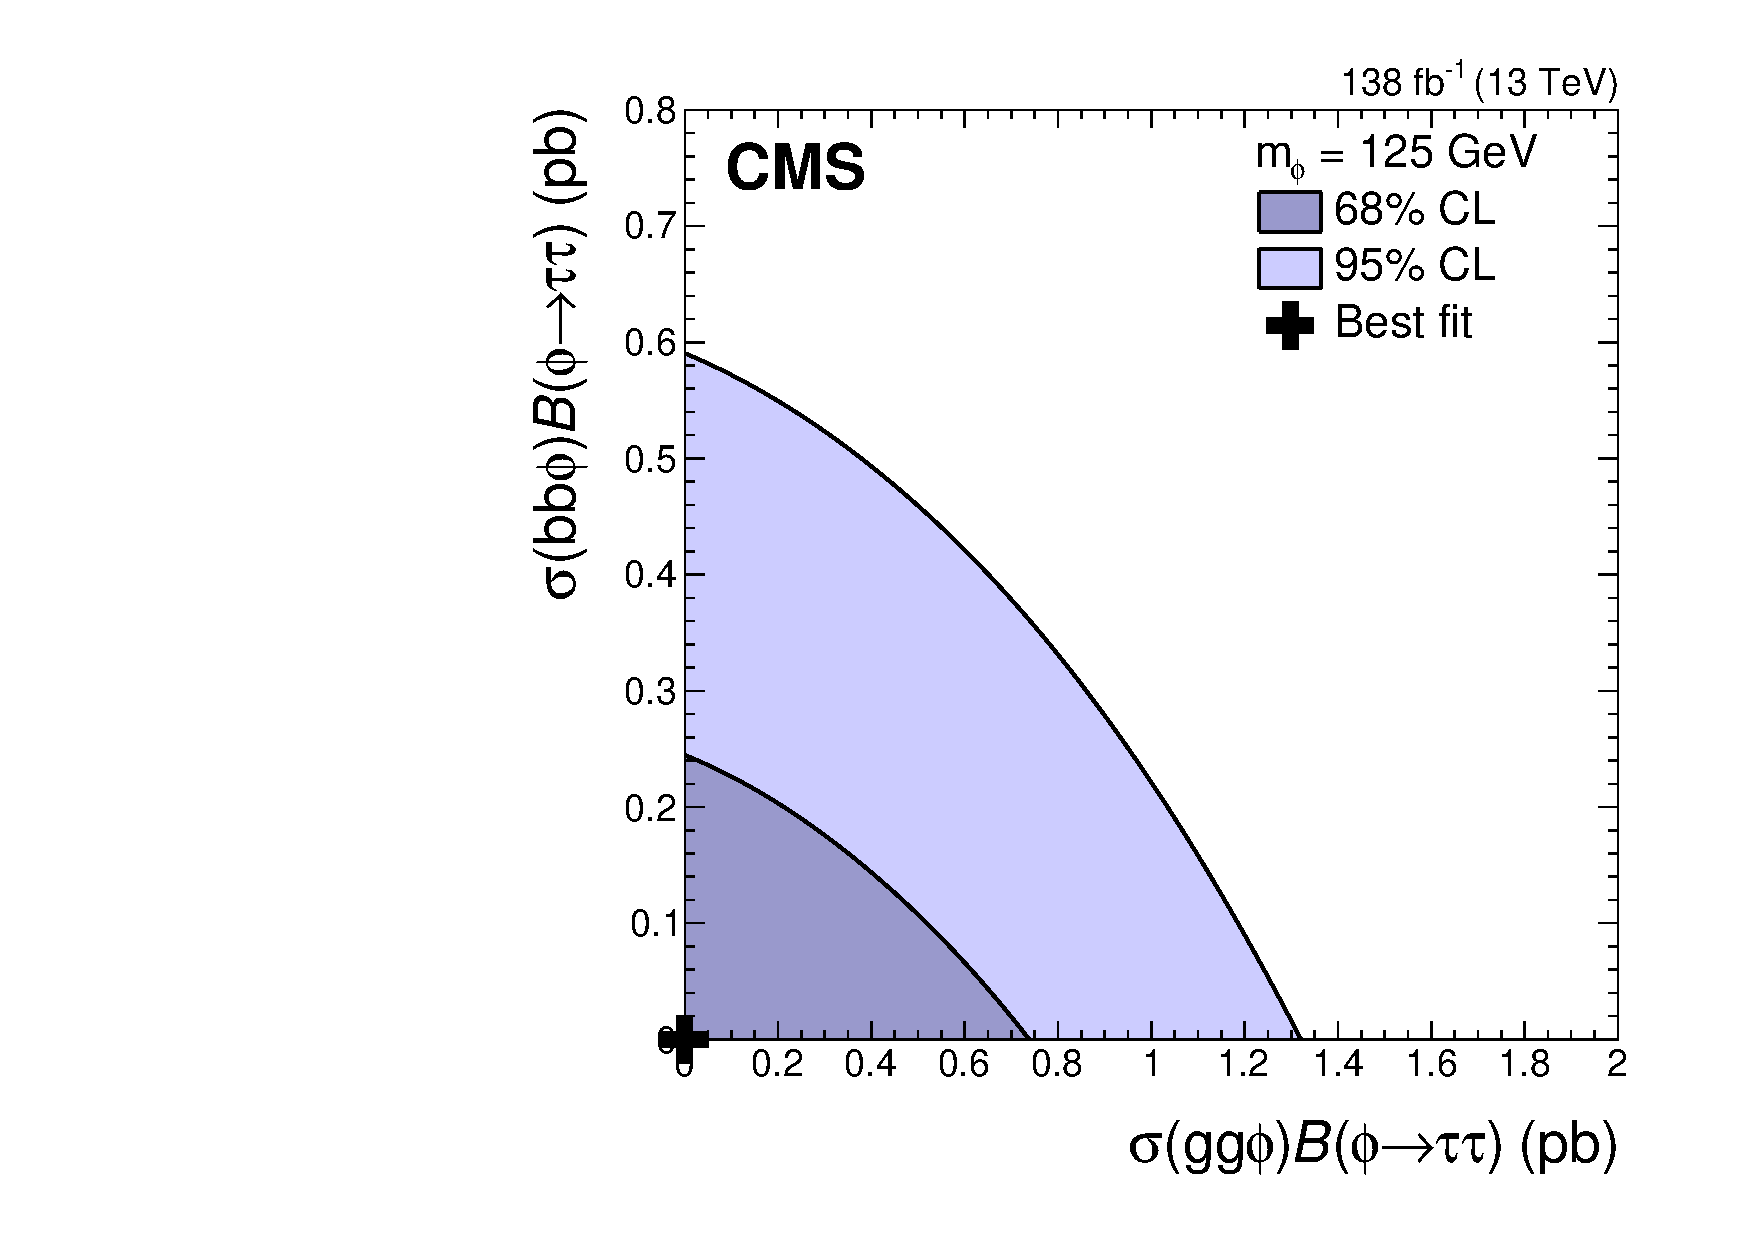
\includegraphics[width=0.33\textwidth]{Figures/2d_lkld_125.pdf}} \\
    \subfloat[]{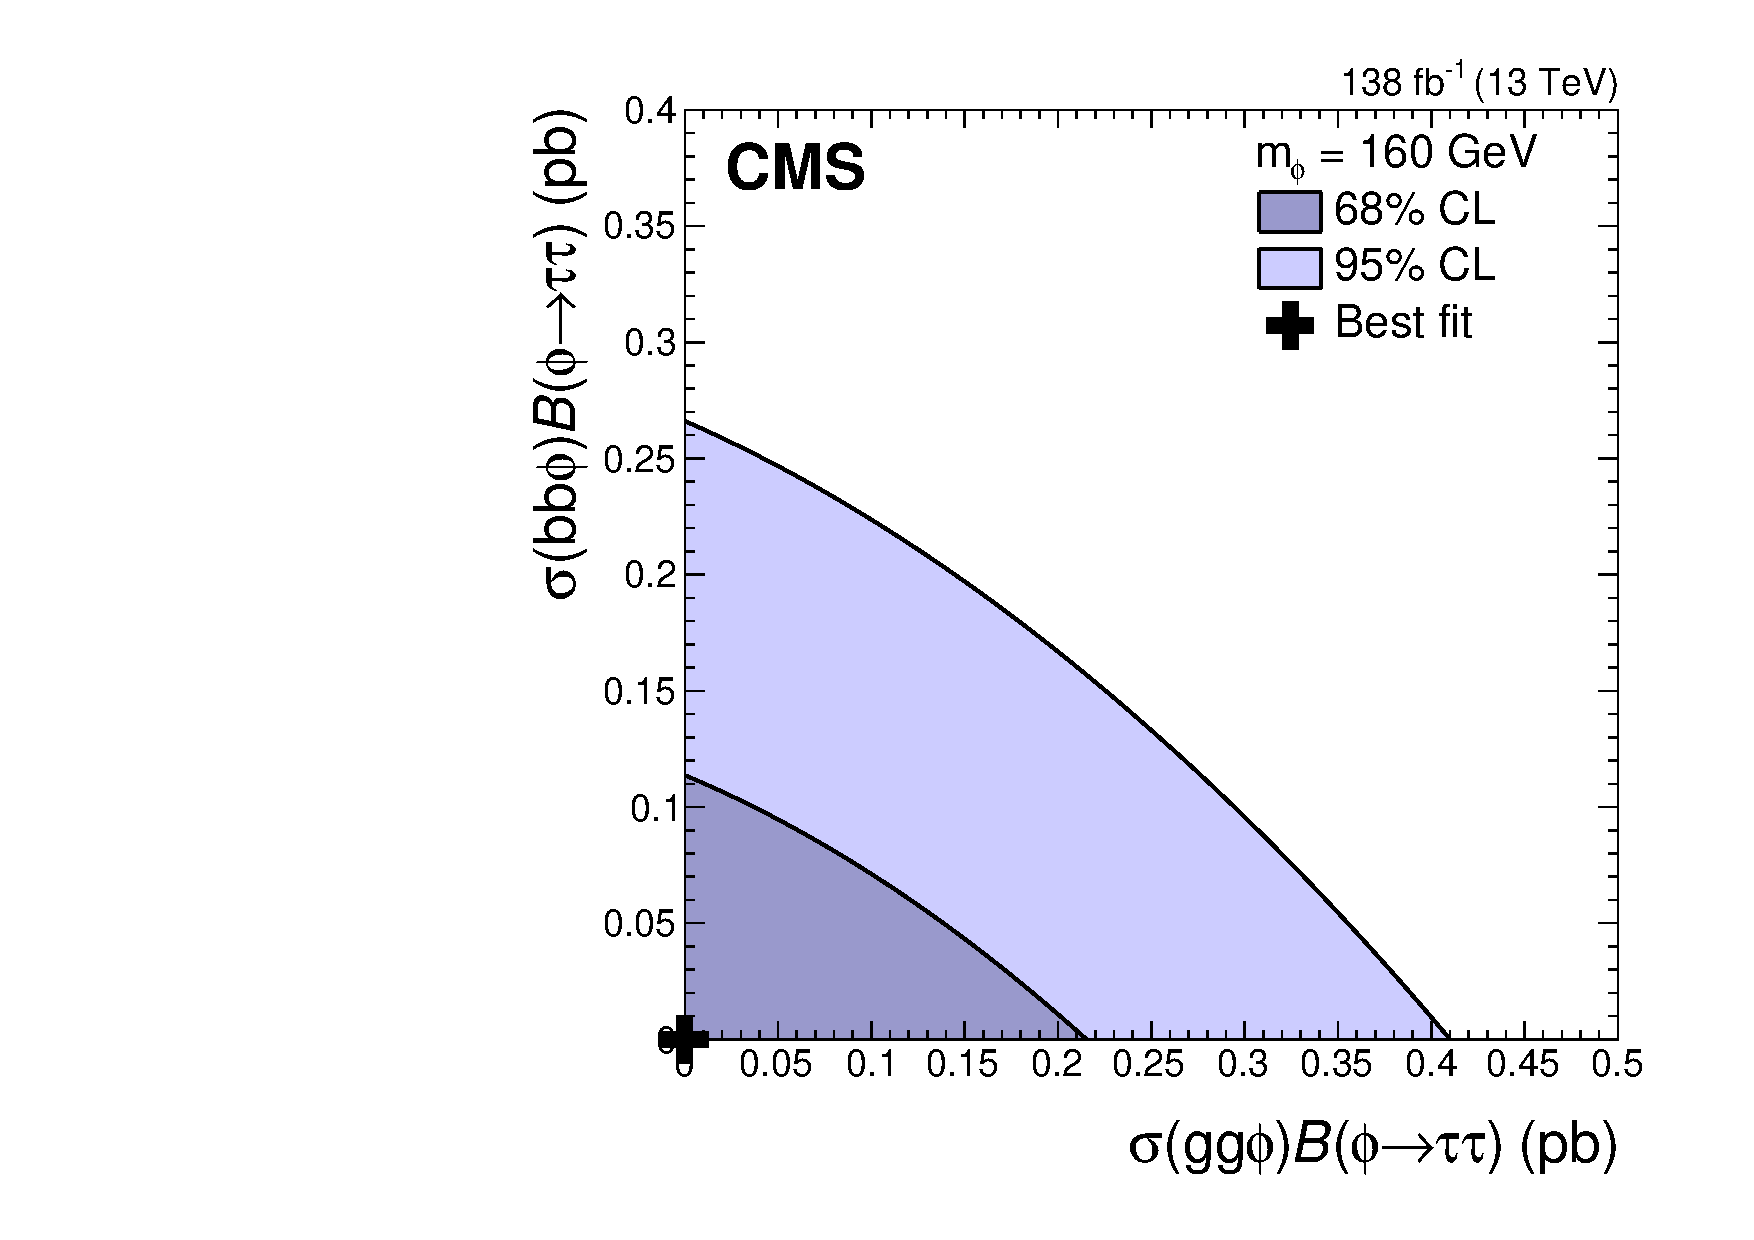
\includegraphics[width=0.33\textwidth]{Figures/2d_lkld_160.pdf}}
    \subfloat[]{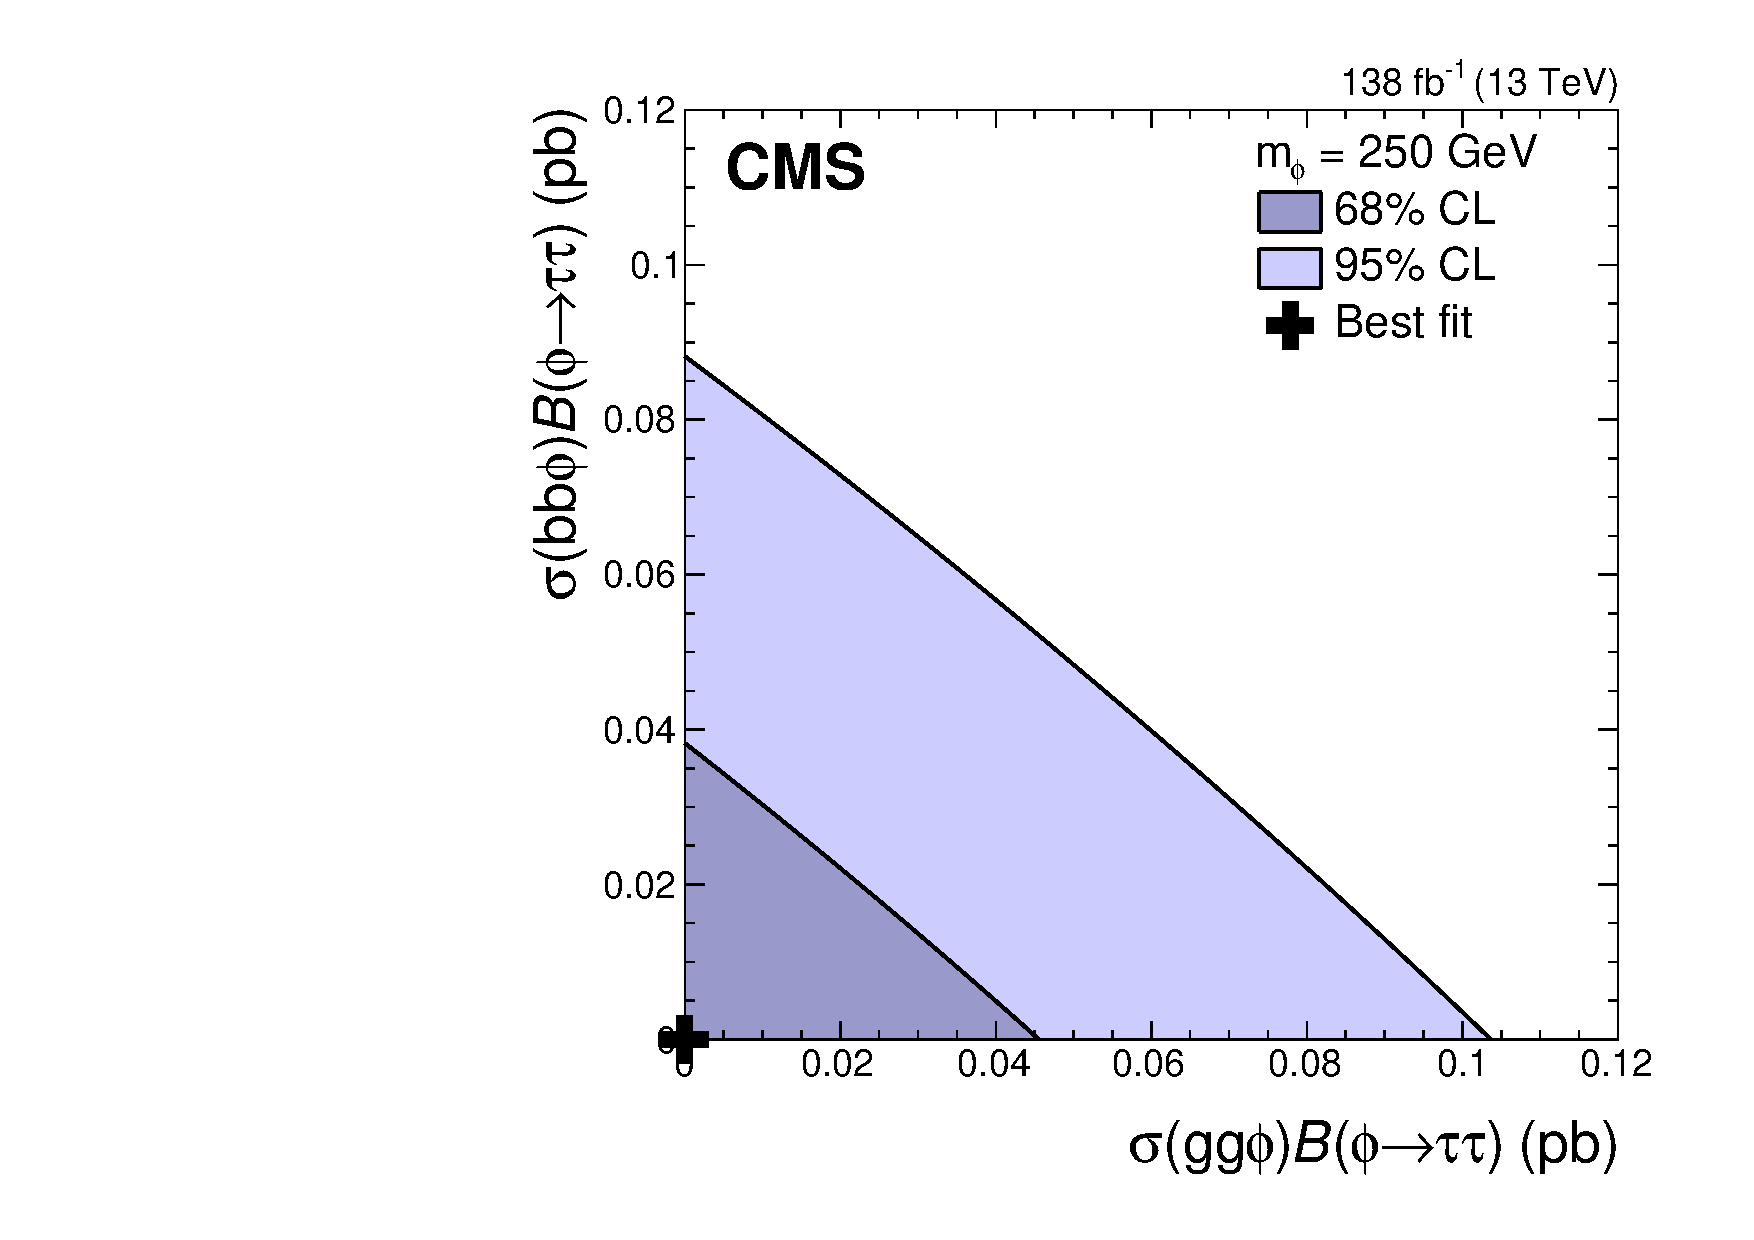
\includegraphics[width=0.33\textwidth]{Figures/2d_lkld_250.pdf}}
    \subfloat[]{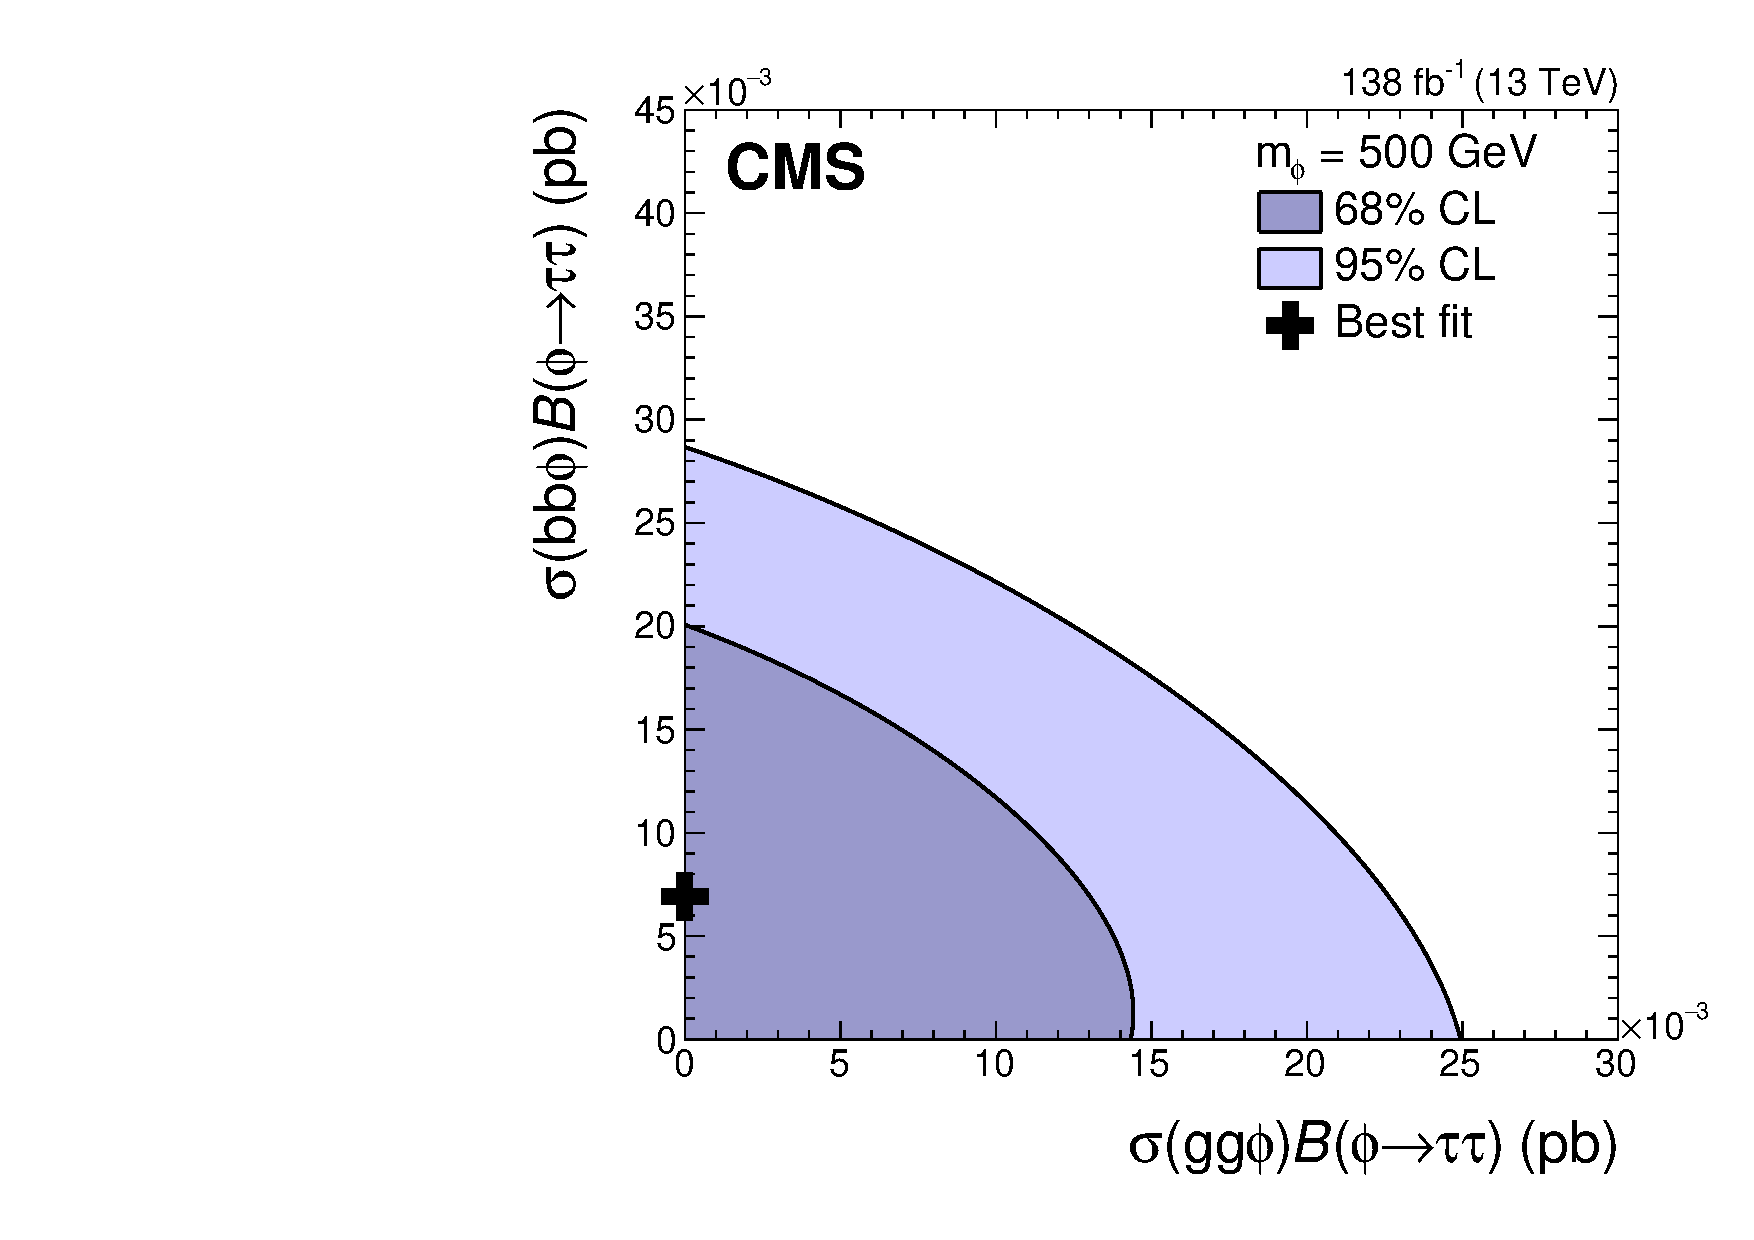
\includegraphics[width=0.33\textwidth]{Figures/2d_lkld_500.pdf}} \\
    \subfloat[]{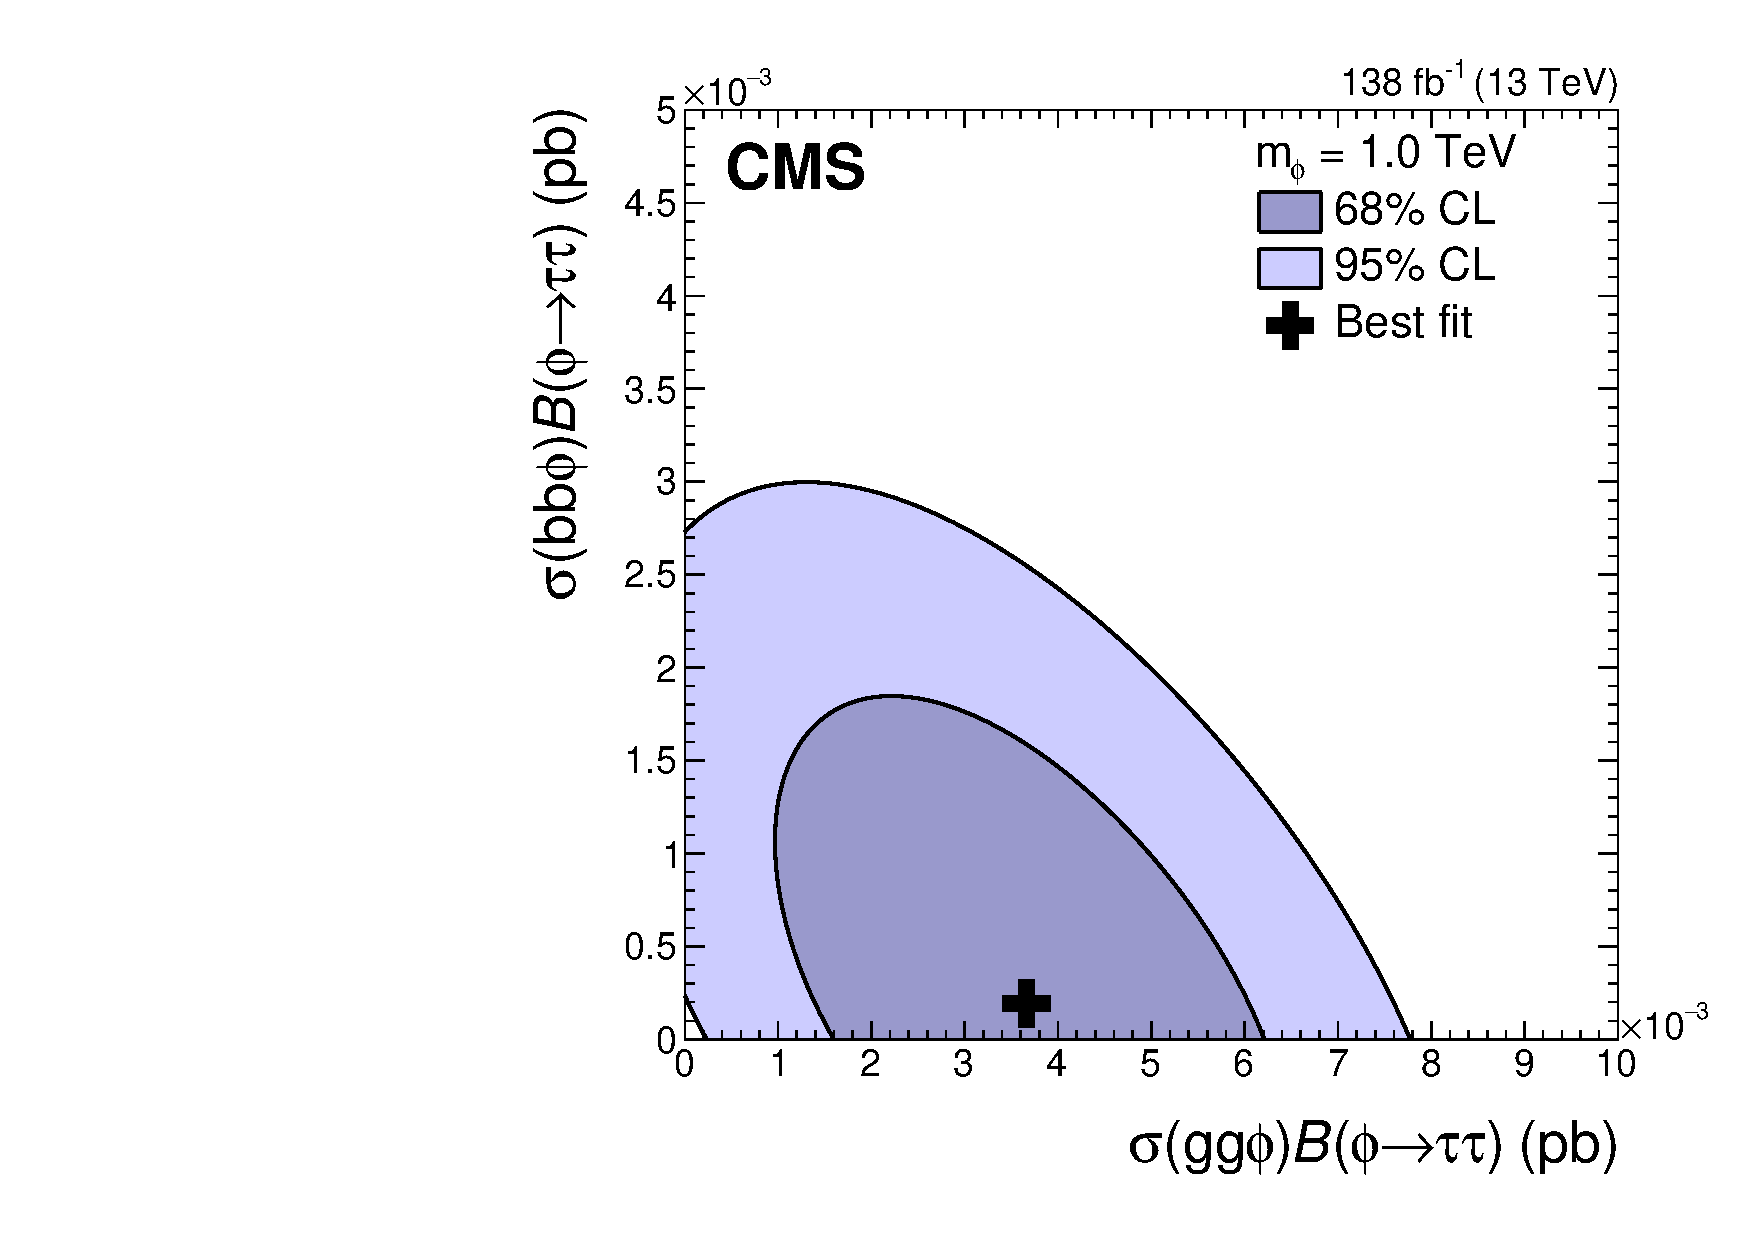
\includegraphics[width=0.33\textwidth]{Figures/2d_lkld_1000.pdf}}
    \subfloat[]{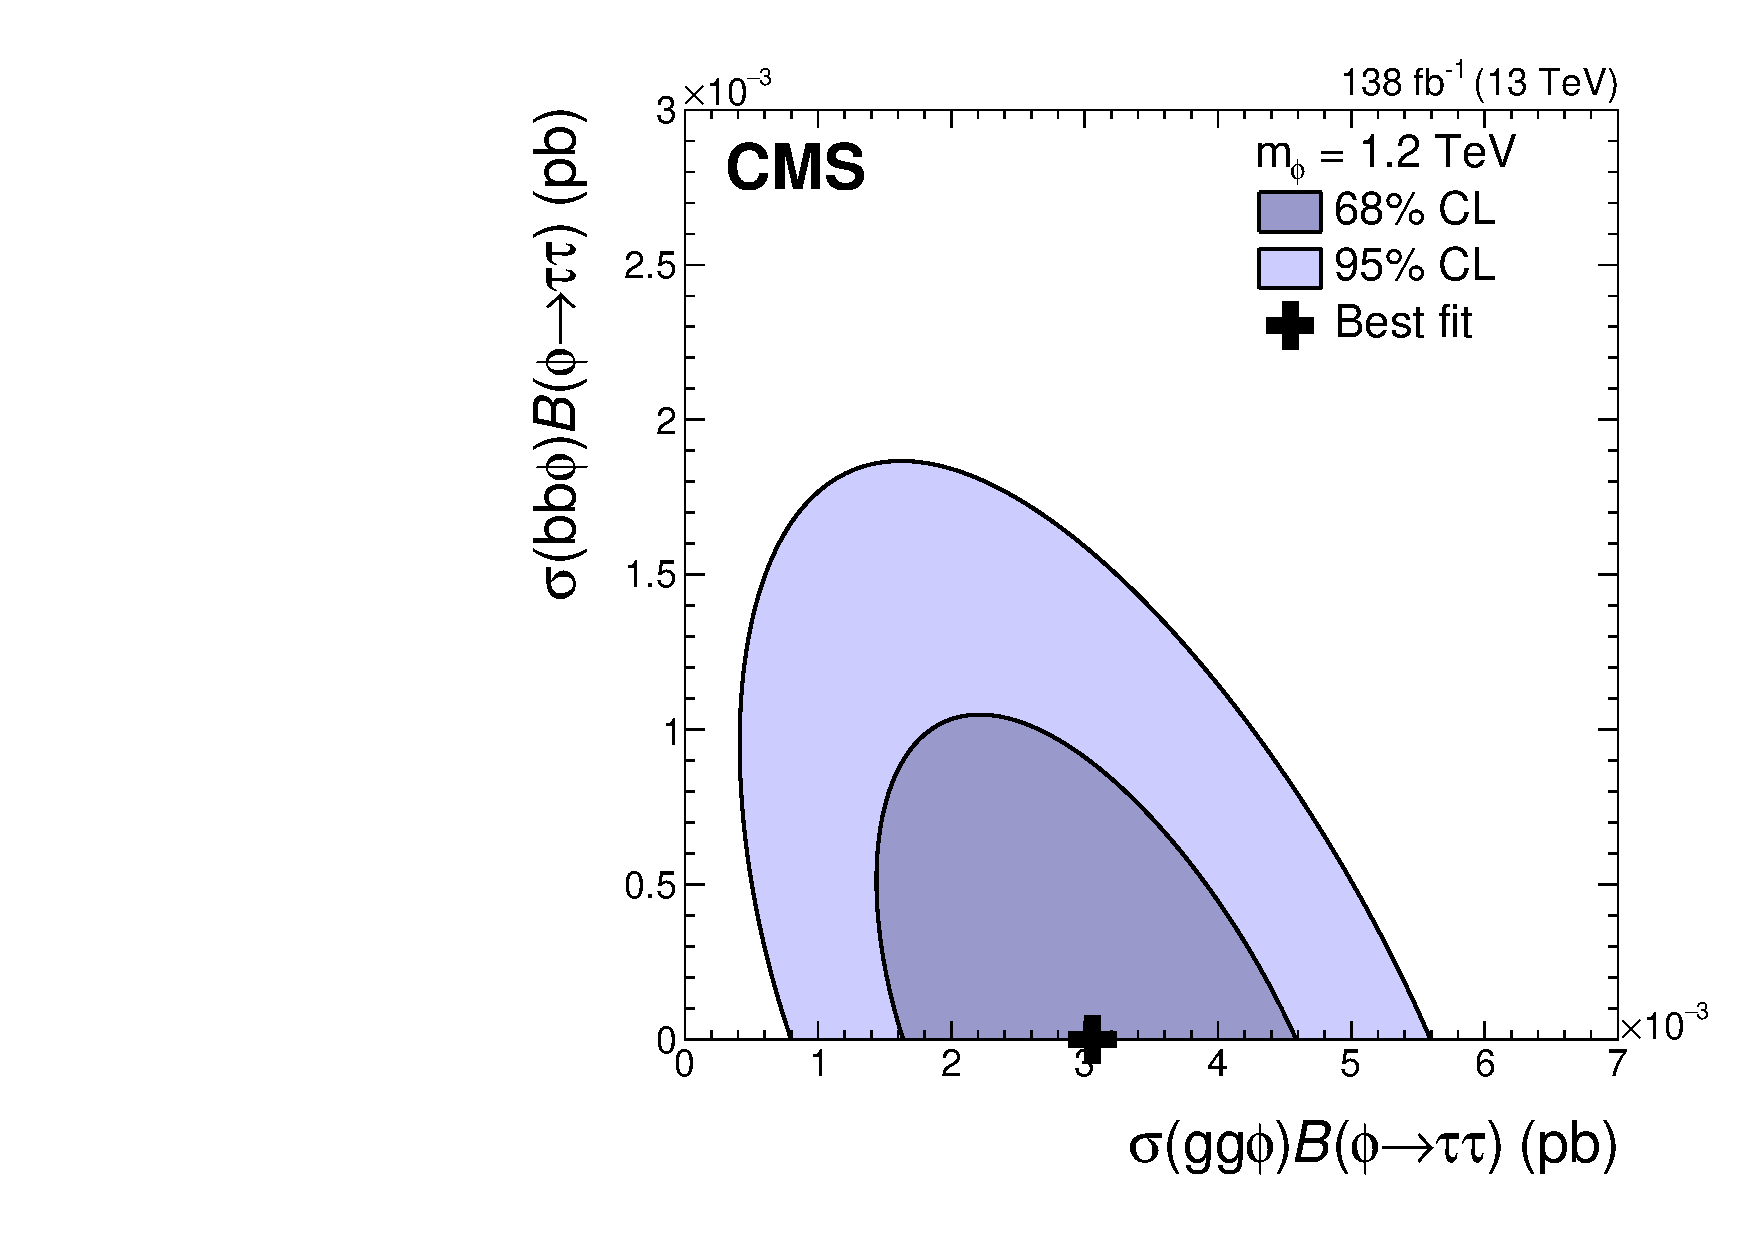
\includegraphics[width=0.33\textwidth]{Figures/2d_lkld_1200.pdf}}
    \subfloat[]{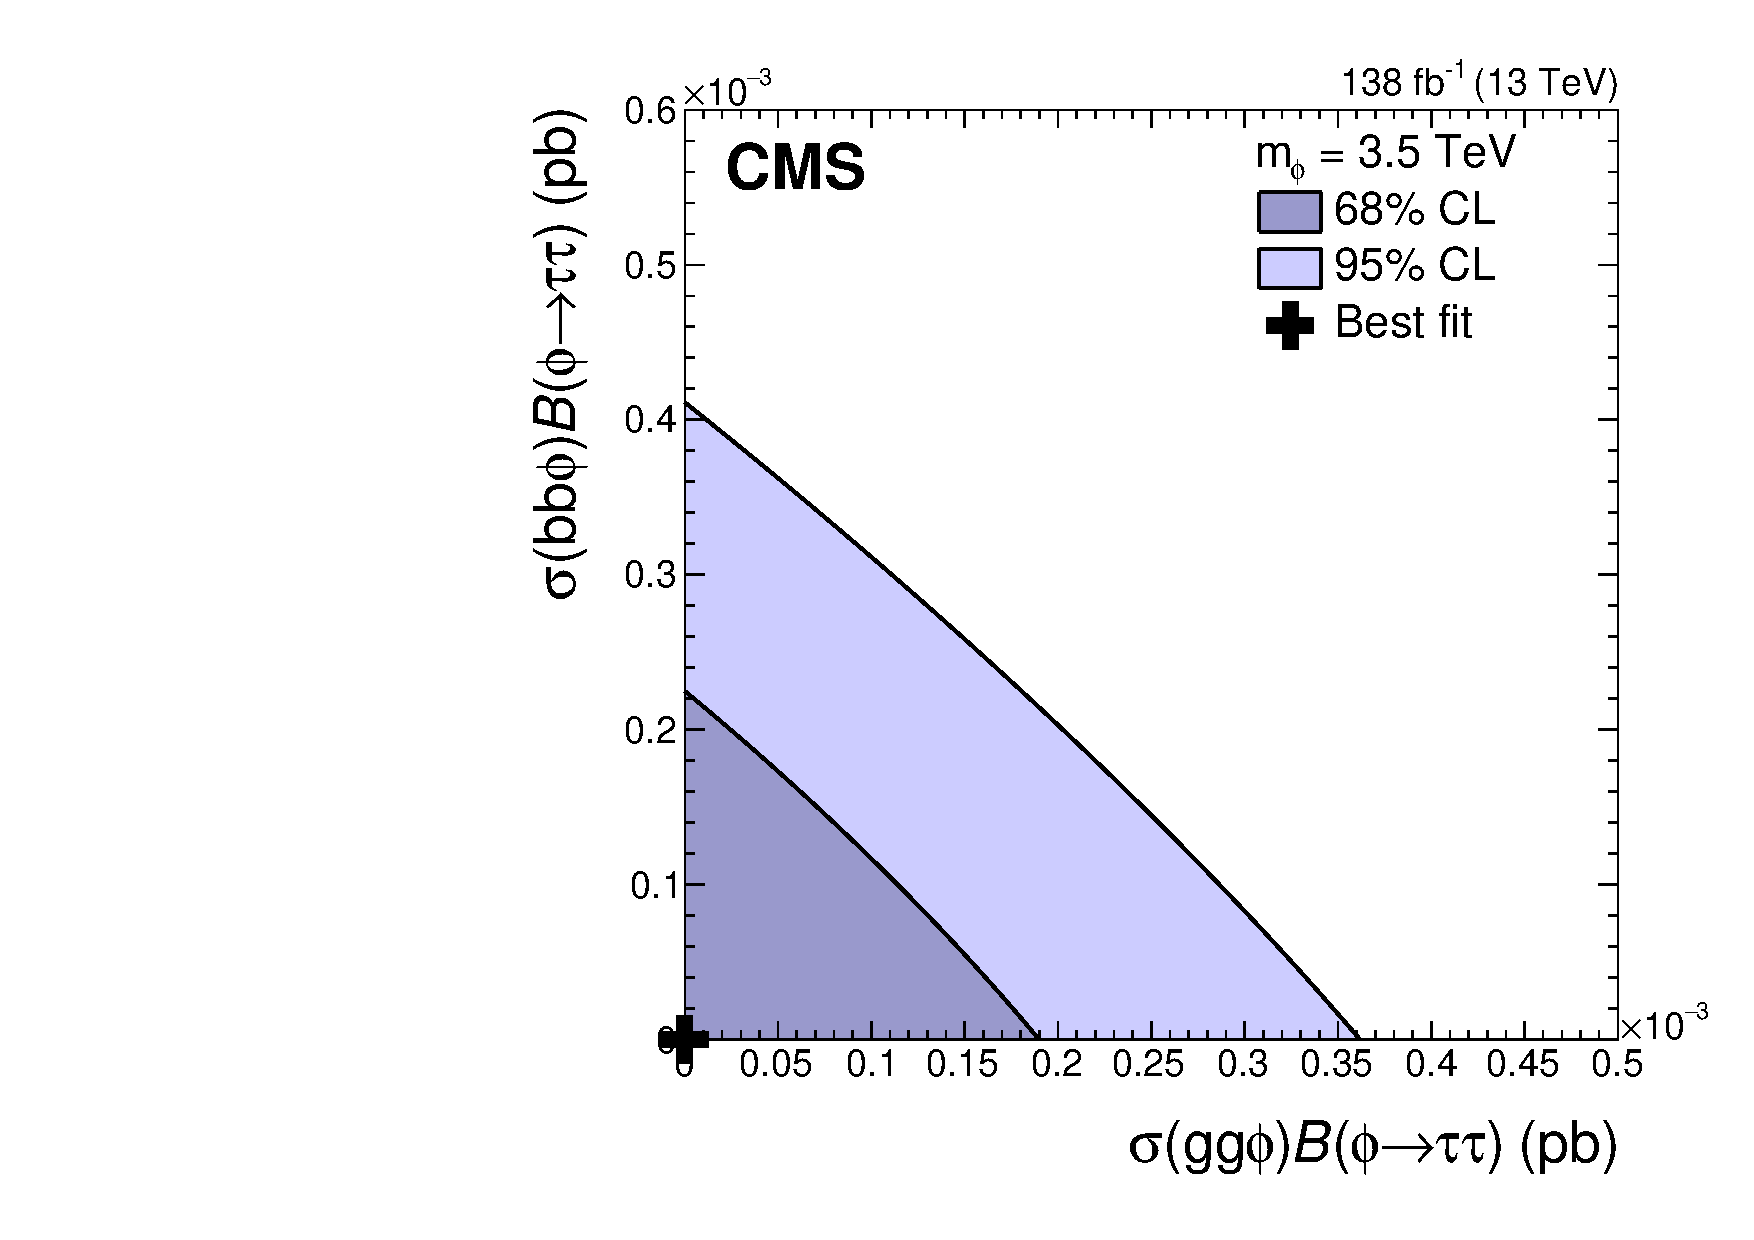
\includegraphics[width=0.33\textwidth]{Figures/2d_lkld_3500.pdf}}
\caption{2D Likelihood scans.}
\label{fig:2d_likelihood_scans}
\end{figure}

\section{Model Dependent Limits}

\subsection{Limit Setting}

\begin{figure}[!hbtp]
\centering
    \subfloat[]{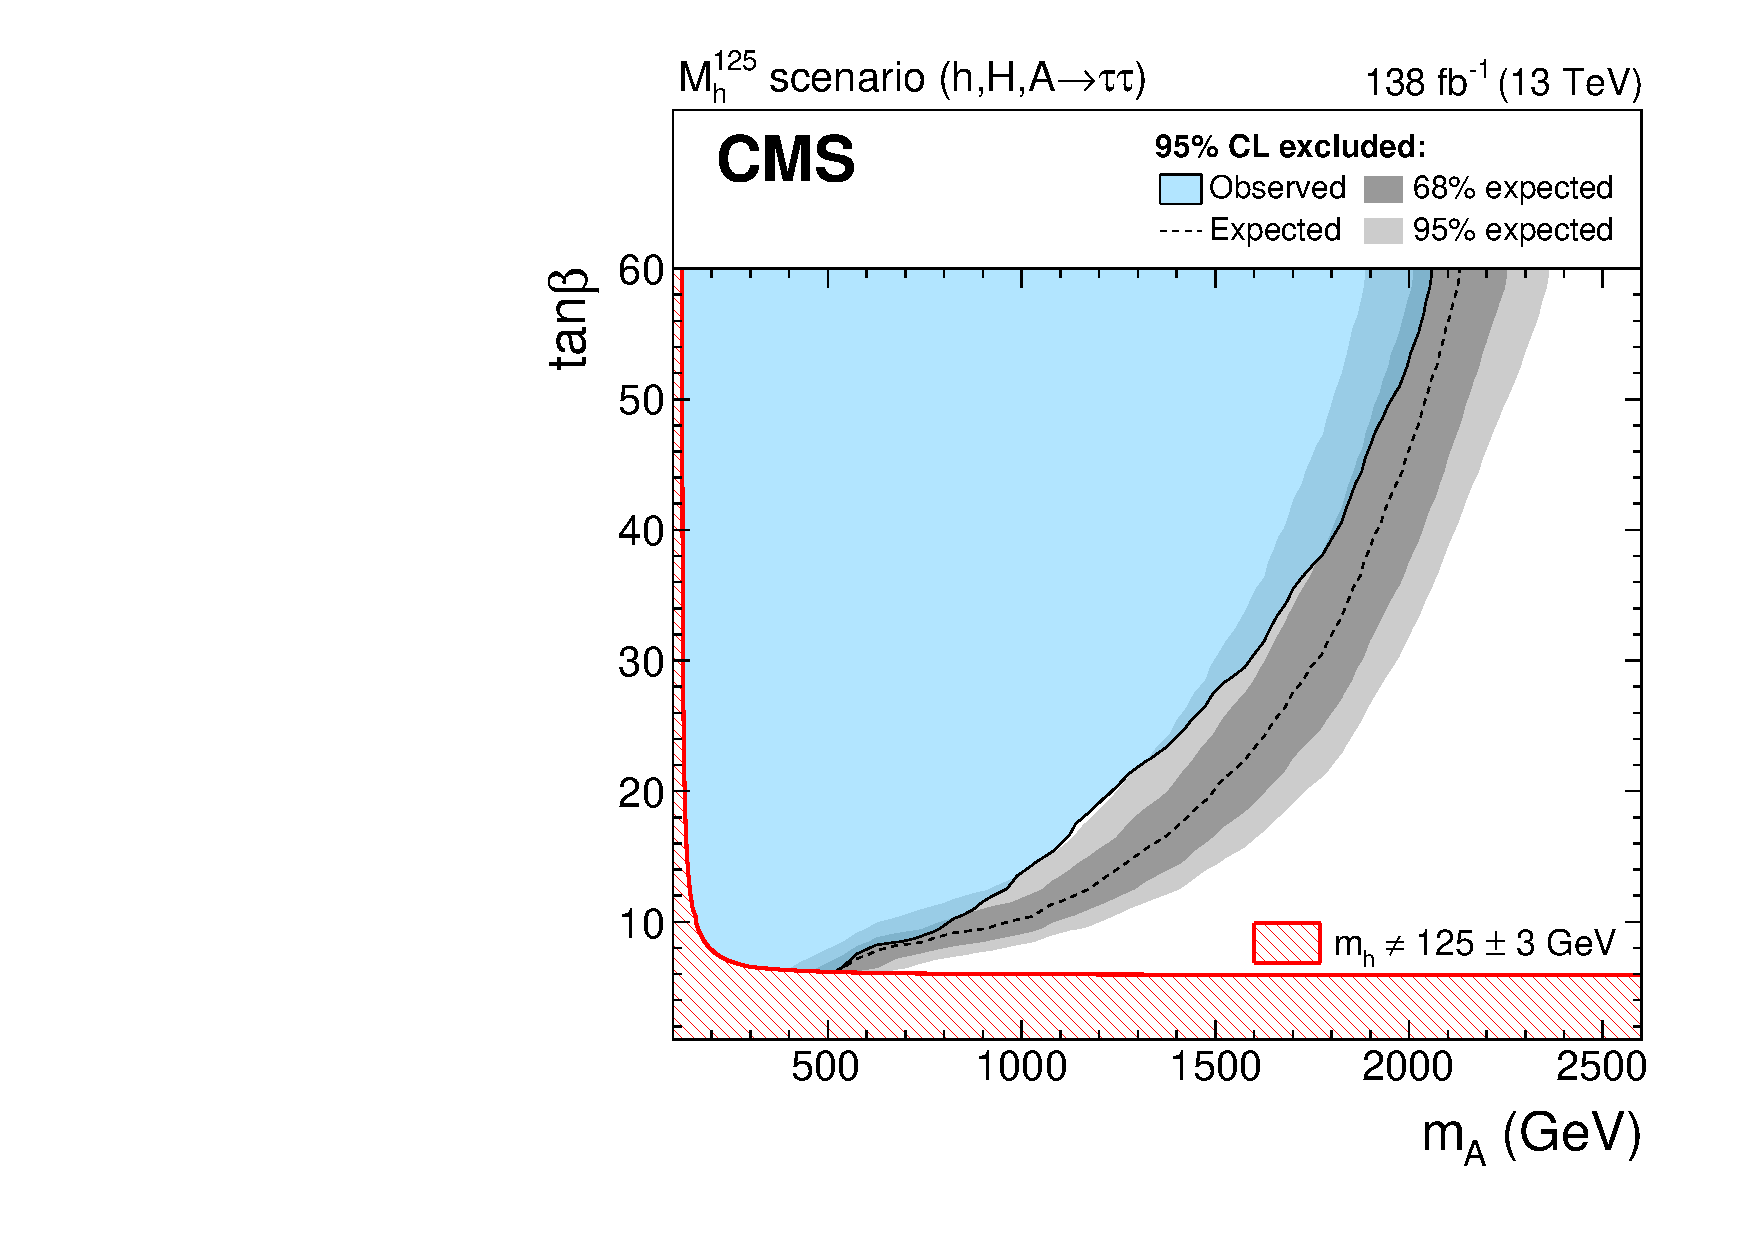
\includegraphics[width=0.5\textwidth]{Figures/model-dependent_limit_mh125.pdf}}
    \subfloat[]{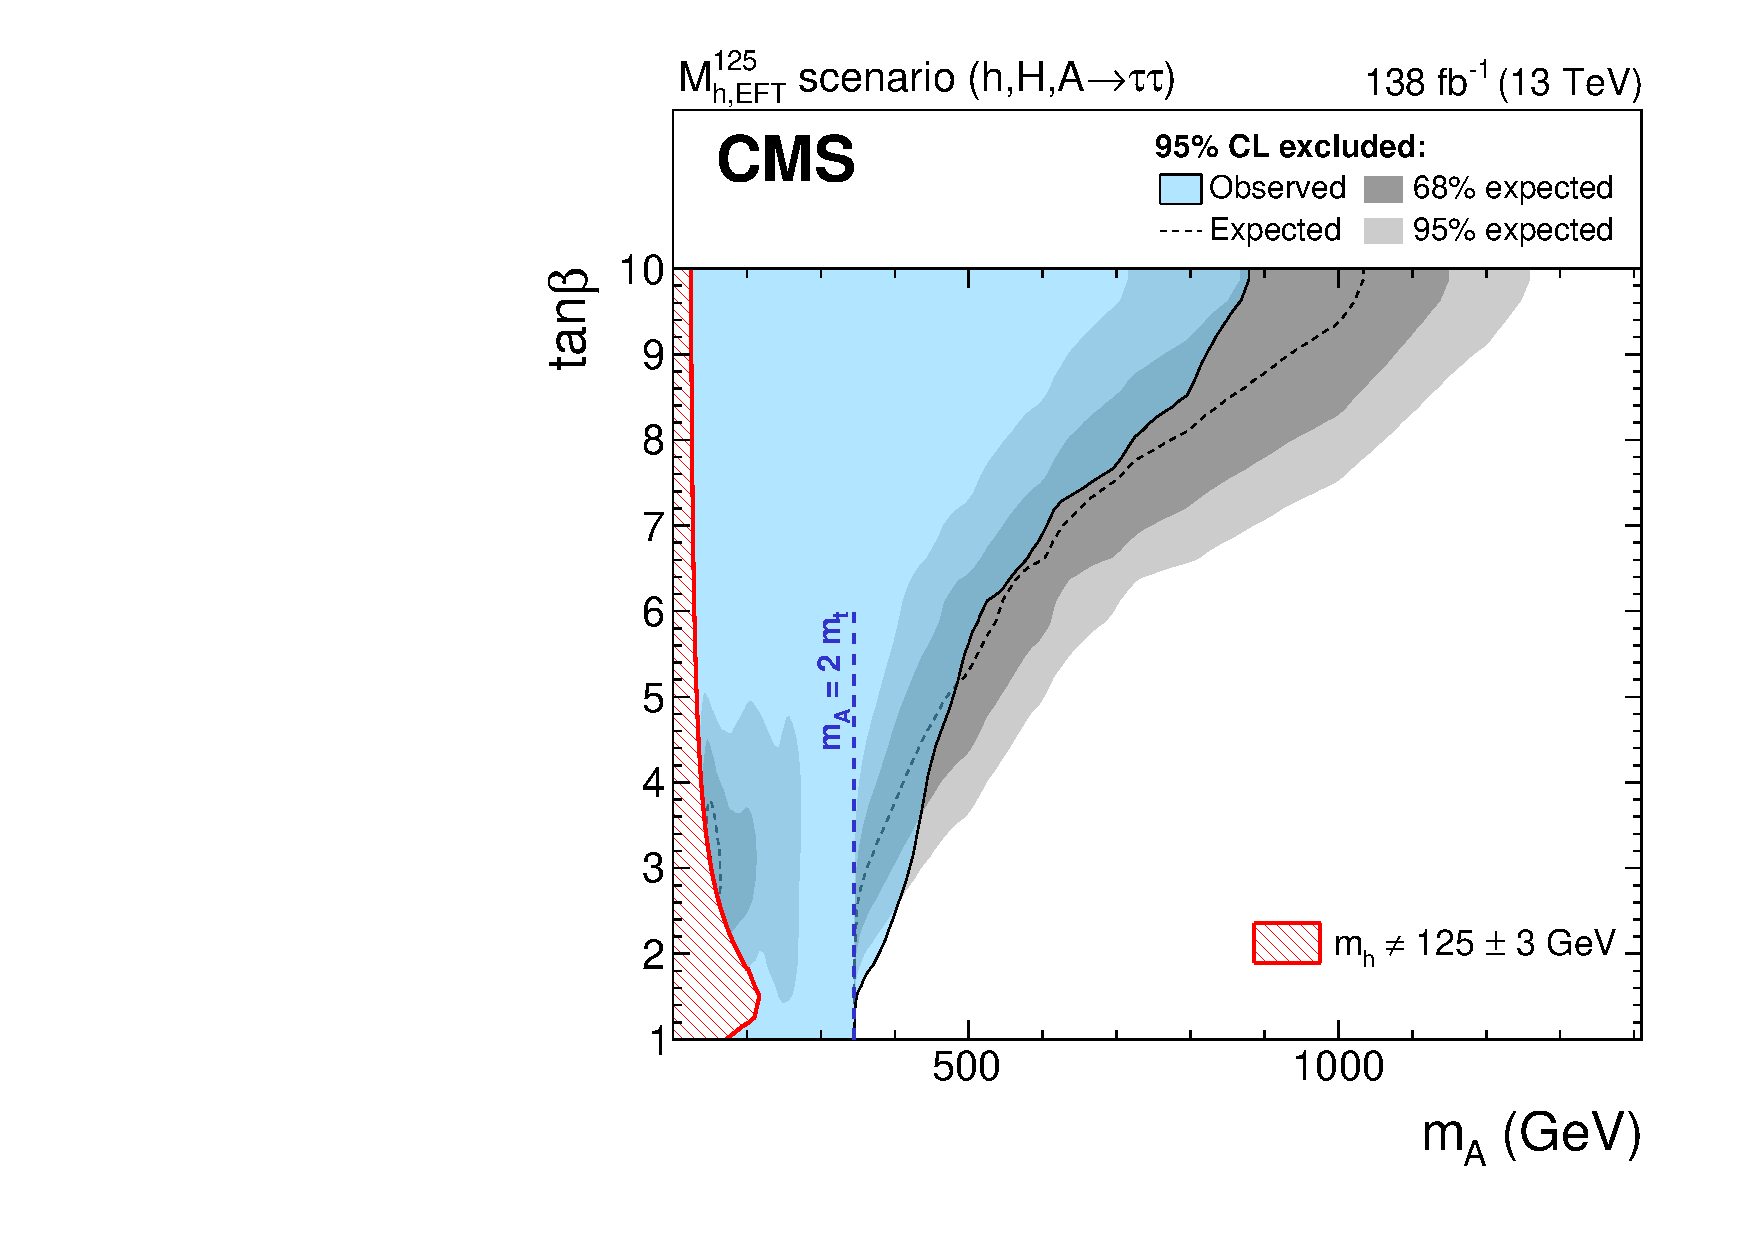
\includegraphics[width=0.5\textwidth]{Figures/model-dependent_limit_mh125EFT.pdf}}
\caption{MSSM limits.}
\label{fig:mssm_limits}
\end{figure}

\begin{figure}[!hbtp]
\centering
    \subfloat[]{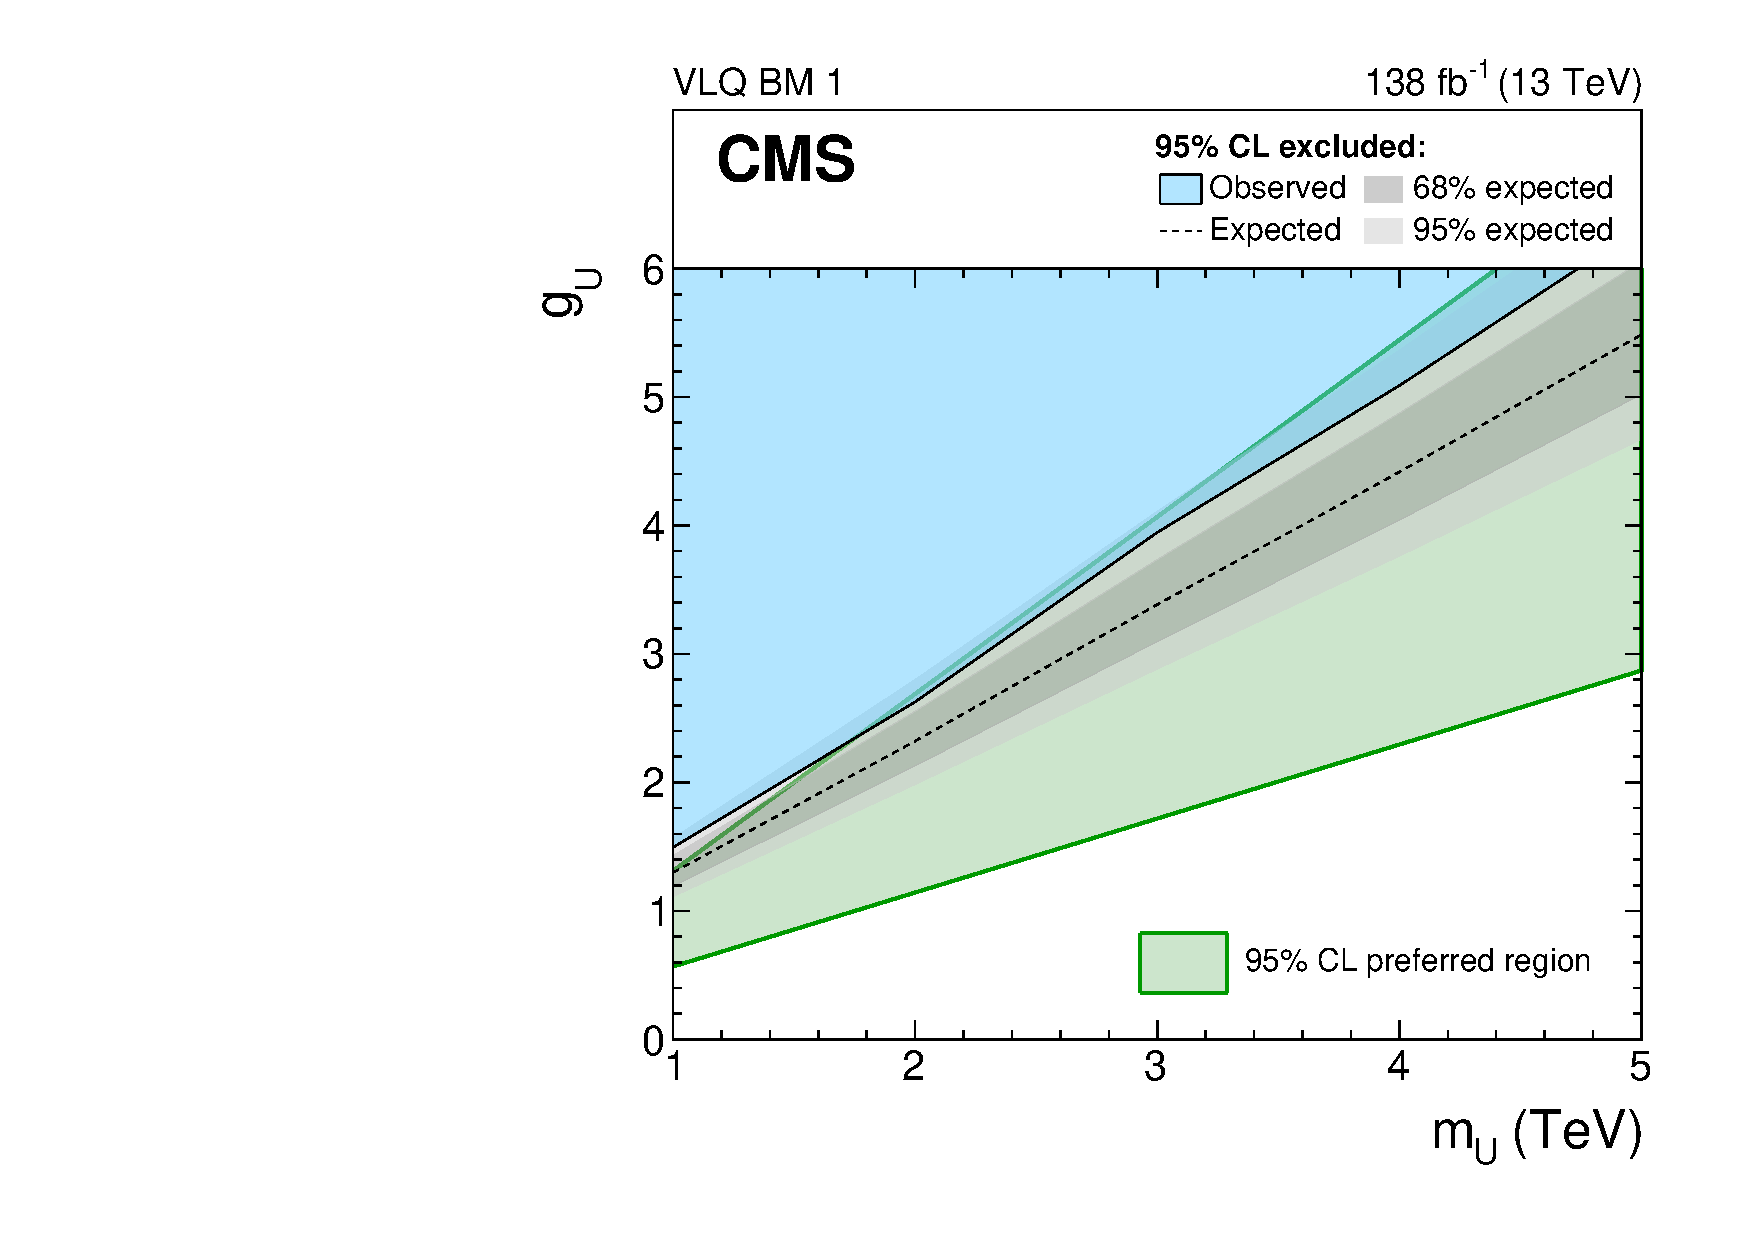
\includegraphics[width=0.5\textwidth]{Figures/vlq_bm_1.pdf}}
    \subfloat[]{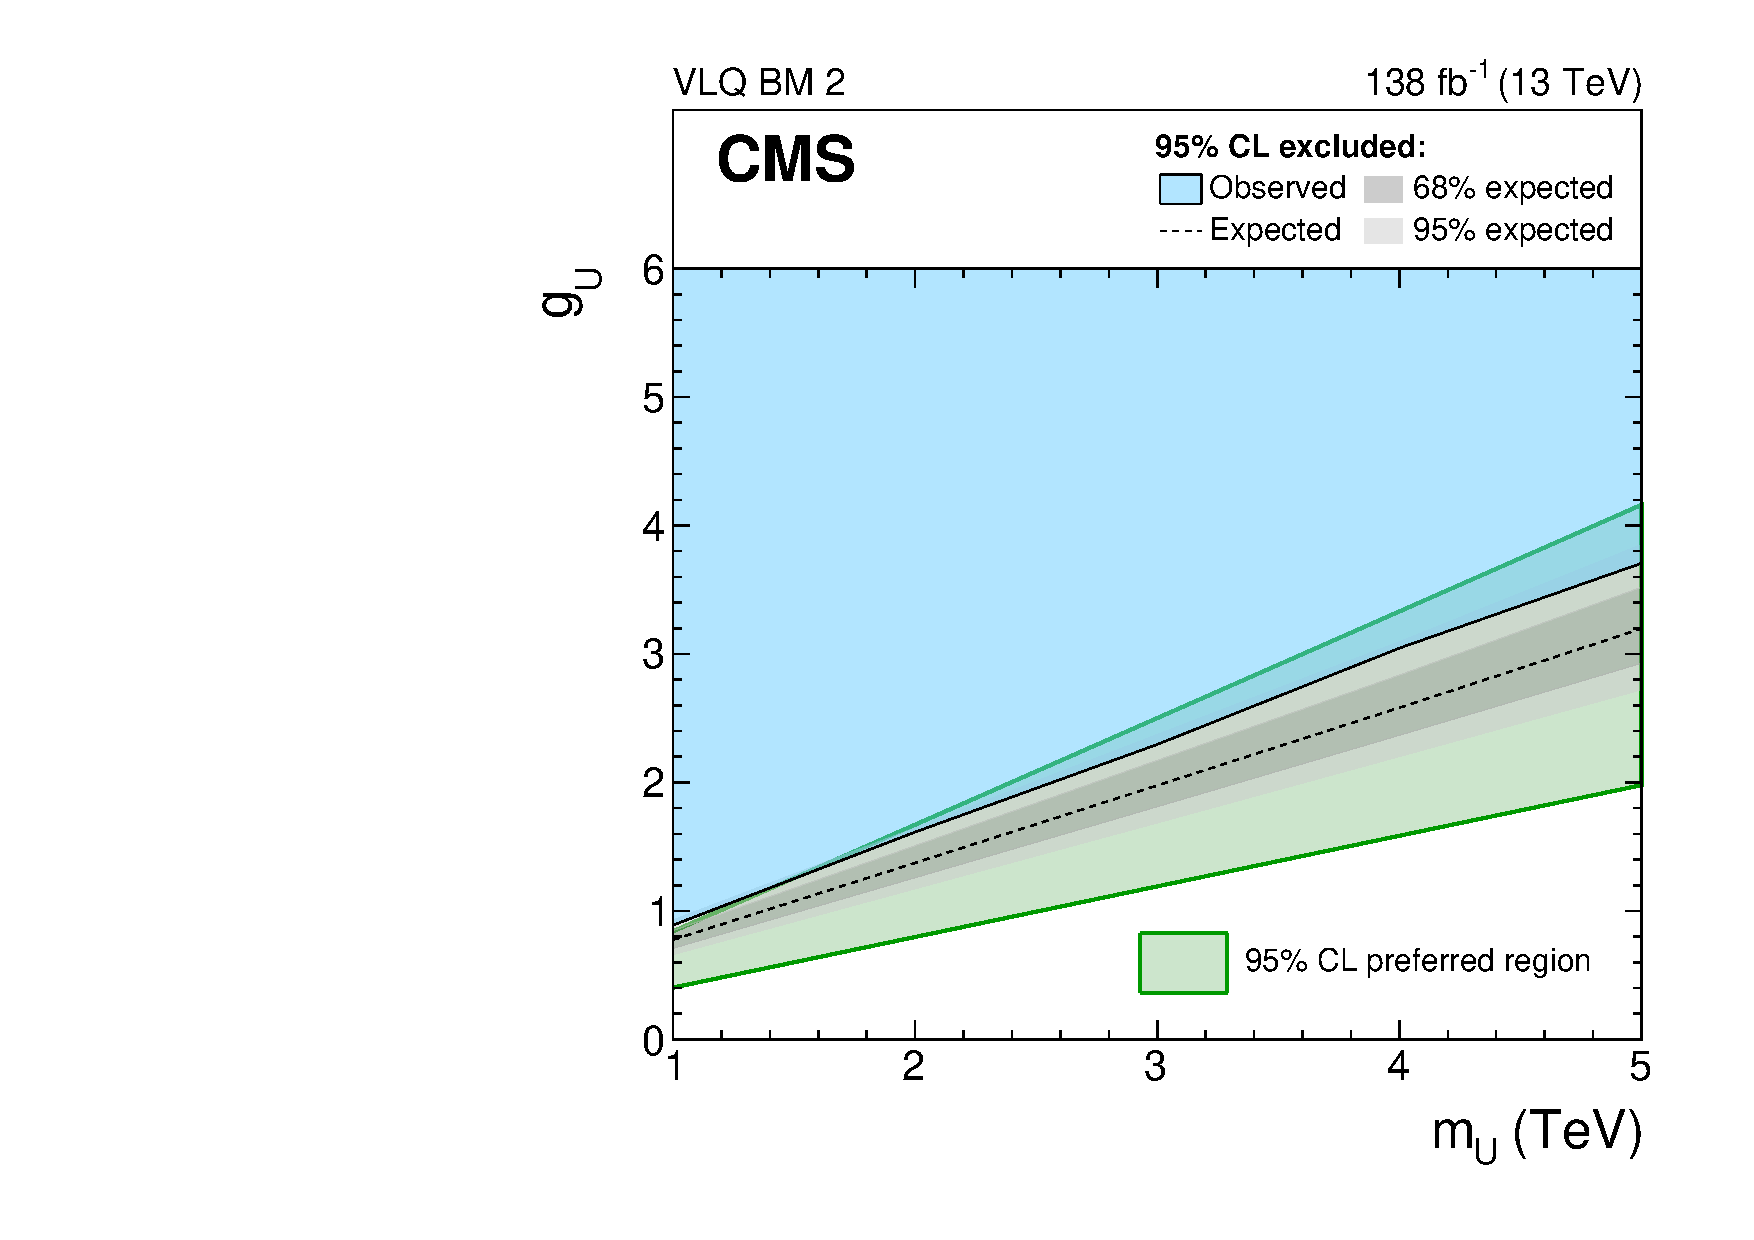
\includegraphics[width=0.5\textwidth]{Figures/vlq_bm_2.pdf}}
\caption{VLQ limits.}
\label{fig:vlq_limits}
\end{figure}

